\documentclass[manuscript,acmsmall,anonymous,review,screen,nonacm=true, authorversion=true]{acmart}

%%
%% \BibTeX command to typeset BibTeX logo in the docs
\AtBeginDocument{%
  \providecommand\BibTeX{{%
    Bib\TeX}}}


\setcopyright{acmcopyright}
\copyrightyear{2018}
\acmYear{2018}
\acmDOI{XXXXXXX.XXXXXXX}

%% These commands are for a PROCEEDINGS abstract or paper.
\acmConference[Conference acronym 'XX]{Make sure to enter the correct
  conference title from your rights confirmation emai}{June 03--05,
  2018}{Woodstock, NY}
%%
%%  Uncomment \acmBooktitle if the title of the proceedings is different
%%  from ``Proceedings of ...''!
%%
%%\acmBooktitle{Woodstock '18: ACM Symposium on Neural Gaze Detection,
%%  June 03--05, 2018, Woodstock, NY}
\acmPrice{15.00}
\acmISBN{978-1-4503-XXXX-X/18/06}


%%
%% Submission ID.
%% Use this when submitting an article to a sponsored event. You'll
%% receive a unique submission ID from the organizers
%% of the event, and this ID should be used as the parameter to this command.
%%\acmSubmissionID{123-A56-BU3}

%%
%% For managing citations, it is recommended to use bibliography
%% files in BibTeX format.
%%
%% You can then either use BibTeX with the ACM-Reference-Format style,
%% or BibLaTeX with the acmnumeric or acmauthoryear sytles, that include
%% support for advanced citation of software artefact from the
%% biblatex-software package, also separately available on CTAN.
%%
%% Look at the sample-*-biblatex.tex files for templates showcasing
%% the biblatex styles.
%%

%%
%% The majority of ACM publications use numbered citations and
%% references.  The command \citestyle{authoryear} switches to the
%% "author year" style.
%%
%% If you are preparing content for an event
%% sponsored by ACM SIGGRAPH, you must use the "author year" style of
%% citations and references.
%% Uncommenting
%% the next command will enable that style.
%%\citestyle{acmauthoryear}
\usepackage{booktabs}   %% For formal tables:
                        %% http://ctan.org/pkg/booktabs
\usepackage{subcaption} %% For complex figures with subfigures/subcaptions
                        %% http://ctan.org/pkg/subcaption

%%%%%%%%%%%%%%%%%%%%%%%%%%%% INPUTTING SELF DEFINED COMMANDS, SELF IMPORTED PACKAGES %%%%%%%%%%%%%%%%%%%%%%%%%%%%%%%%%%%%%%%%%%

%%%%%%%%%%%%%%%%%%%%%%%%%%%% FINISHING INPUTTING SELF DEFINED COMMANDS, SELF IMPORTED PACKAGES %%%%%%%%%%%%%%%%%%%%%%%%%%%%%%%%%%%%%%%%%%
%%


\usepackage[T1]{fontenc}
\usepackage[normalem]{ulem}
\usepackage{mathtools}
\usepackage{blkarray,bigstrut} 
\usepackage{graphicx,wrapfig,lipsum}
\usepackage{tcolorbox}
\usepackage{enumitem}
\usepackage{array}
\usepackage{algorithm}
\usepackage{algorithmic}
\usepackage{mathpartir}
\usepackage{multirow}
\usepackage{hyperref}
\usepackage{amssymb}
\usepackage{subcaption}
\usepackage{stmaryrd}
\usepackage{color} 


\usepackage{tikz}
\usetikzlibrary{snakes}
\usetikzlibrary{svg.path} 
\usetikzlibrary{calc} 
\usetikzlibrary{shapes}
\usetikzlibrary{shapes.geometric}
\usetikzlibrary{arrows.meta}
\usetikzlibrary{arrows}
\usetikzlibrary{decorations.text,decorations.markings}
% % % % 

%%%%%%%%%%Packages for adaoption%%%

% \usepackage{amsthm} 

%Packages

%%%%%%%%%%%%%%%%%%%%%%%%%%%%%%%%%%%%%%%%%%%%%%%%%%%%%%%%%%%%%%%%%%%%%%%%%%%%%%%%%%%%%%%%%%%%%%%%%%%%%%%%%%%%%%%%%%%%%%%%%%%%%%%%%%%%%%%%%
%%%%%%%%%%%%%%%%%%%%%%%%%%%%%%%%%%%%%%%%%%%%%%%%%%%%% COMMANDS FOR GENERAL PAPER WRITING %%%%%%%%%%%%%%%%%%%%%%%%%%%%%%%%%%%%%%%%%%%%%%%%%%%%
%%%%%%%%%%%%%%%%%%%%%%%%%%%%%%%%%%%%%%%%%%%%%%%%%%%%%%%%%%%%%%%%%%%%%%%%%%%%%%%%%%%%%%%%%%%%%%%%%%%%%%%%%%%%%%%%%%%%%%%%%%%%%%%%%%%%%%%%%

%%%%%%%%%%%%%%%%%% LINK STYLE:
\hypersetup{
  colorlinks=true,
  linkcolor=blue!50!red,
  urlcolor=green!70!black
}

%%%%%%%%%%%%%%%%%%%%%%%%%%%% Theorem, Definition and Proof
\newtheorem{lem}{Lemma}[section]
\newtheorem{thm}{Theorem}[section]
\newtheorem{defn}{Definition}
\newtheorem{coro}{Corollary}[thm]

\newtheorem{example}{Example}[section]

\newcommand{\todo}[1]{{\color{red}\textbf{[[ #1 ]]}}}
\newcommand{\todomath}[1]{{\scriptstyle \color{red}\mathbf{[[ #1 ]]}}}
\newcommand{\completeness}[1]{{\color{blue}\textbf{[[ #1 ]]}}}
\newcommand{\caseL}[1]{\item \textbf{case: #1}\newline}
\newcommand{\subcaseL}[1]{\item \textbf{sub-case: #1}\newline}
\newcommand{\subsubcaseL}[1]{\item \textbf{subsub-case: #1}\newline}
\newcommand{\subsubsubcaseL}[1]{\item \textbf{subsubsub-case: \boldmath{#1}}\newline}

\newcommand{\blue}[1]{{\tiny \color{blue}{ #1 }}}


\let\originalleft\left
\let\originalright\right
\renewcommand{\left}{\mathopen{}\mathclose\bgroup\originalleft}
\renewcommand{\right}{\aftergroup\egroup\originalright}
\newcommand{\ts}[1]{ \llparenthesis {#1} \rrparenthesis }

\theoremstyle{definition}

\newtheorem{case}{Case}
\newtheorem{subcase}{Case}
\numberwithin{subcase}{case}
\newtheorem{subsubcase}{Case}
\numberwithin{subsubcase}{subcase}

\newtheorem{subsubsubcase}{Case}
\numberwithin{subsubsubcase}{subsubcase}
\newcommand{\st}{~.~}

%%%%COLORS
\definecolor{periwinkle}{rgb}{0.8, 0.8, 1.0}
\definecolor{powderblue}{rgb}{0.69, 0.88, 0.9}
\definecolor{sandstorm}{rgb}{0.93, 0.84, 0.25}
\definecolor{trueblue}{rgb}{0.0, 0.45, 0.81}

\newlength\Origarrayrulewidth
% horizontal rule equivalent to \cline but with 2pt width
\newcommand{\Cline}[1]{%
 \noalign{\global\setlength\Origarrayrulewidth{\arrayrulewidth}}%
 \noalign{\global\setlength\arrayrulewidth{2pt}}\cline{#1}%
 \noalign{\global\setlength\arrayrulewidth{\Origarrayrulewidth}}%
}

% draw a vertical rule of width 2pt on both sides of a cell
\newcommand\Thickvrule[1]{%
  \multicolumn{1}{!{\vrule width 2pt}c!{\vrule width 2pt}}{#1}%
}

% draw a vertical rule of width 2pt on the left side of a cell
\newcommand\Thickvrulel[1]{%
  \multicolumn{1}{!{\vrule width 2pt}c|}{#1}%
}

% draw a vertical rule of width 2pt on the right side of a cell
\newcommand\Thickvruler[1]{%
  \multicolumn{1}{|c!{\vrule width 2pt}}{#1}%
}

\newenvironment{subproof}[1][\proofname]{%
  \renewcommand{\qedsymbol}{$\blacksquare$}%
  \begin{proof}[#1]%
}{%
  \end{proof}%
}
%%%%%%%%%%%%%%%%%%%%%%%%%%%%%%% Fonts Definition %%%%%%%%%%%%%%%%%%%%%%%%%%%
\newcommand{\omitthis}[1]{}

% Misc.
\newcommand{\etal}{\textit{et al.}}
\newcommand{\bump}{\hspace{3.5pt}}

% Text fonts
\newcommand{\tbf}[1]{\textbf{#1}}

% Math fonts
\newcommand{\mbb}[1]{\mathbb{#1}}
\newcommand{\mbf}[1]{\mathbf{#1}}
\newcommand{\mrm}[1]{\mathrm{#1}}
\newcommand{\mtt}[1]{\mathtt{#1}}
\newcommand{\mcal}[1]{\mathcal{#1}}
\newcommand{\mfrak}[1]{\mathfrak{#1}}
\newcommand{\msf}[1]{\mathsf{#1}}
\newcommand{\mscr}[1]{\mathscr{#1}}

\newcommand{\diam}{{\color{red}\diamond}}
\newcommand{\dagg}{{\color{blue}\dagger}}
\let\oldstar\star
\renewcommand{\star}{\oldstar}

\newcommand{\im}[1]{\ensuremath{#1}}

\newcommand{\kw}[1]{\im{\mathtt{#1}}}
\newcommand{\set}[1]{\im{\{{#1}\}}}

\newcommand{\mmax}{\ensuremath{\mathsf{max}}}

\lstnewenvironment{ocaml}[2][]%
  {\lstset{language=ocaml,style=ocaml-pretty,captionpos=t,abovecaptionskip=-\medskipamount,caption={#2},#1}}
  %
  {}

\makeatletter
\newcommand{\mysmallishfont}{\@setfontsize\mysmallishfont{8.7pt}{9.7pt}}
\makeatother

\makeatletter
\newcommand{\myecfont}{\@setfontsize\myecfont{9.7pt}{10.7pt}}
\makeatother

\makeatletter
\newcommand{\myecsmfont}{\@setfontsize\myecfont{8.7pt}{9.7pt}}
\makeatother

\lstdefinelanguage{ocaml}{
  style=ocaml-default,
  keywordsprefix={'},
  morekeywords=[1]{},
  morekeywords=[2]{type,op,axiom,lemma,module,pred,const,declare},
  morekeywords=[3]{var,proc},
  morekeywords=[4]{while,if,then,else,elif,return,proof,qed,realize,rec, match},
}

\lstdefinestyle{ocaml-default}{
  escapechar=\#,
  upquote=true,
  columns=fullflexible,
  captionpos=b,
  frame=tb,
  xleftmargin=0pt,
  xrightmargin=0pt,
  rangebeginprefix={(**\ begin\ },
  rangeendprefix={(**\ end\ },
  rangesuffix={\ *)},
  includerangemarker=false,
  basicstyle=\mysmallishfont\sffamily,
  identifierstyle={},
  keywordstyle=[1]{\itshape},
  keywordstyle=[2]{\bfseries},
  keywordstyle=[3]{\bfseries},
  keywordstyle=[4]{\bfseries},
  keywordstyle=[5]{\bfseries},
  keywordstyle=[6]{\bfseries},
  keywordstyle=[7]{},
  keywordstyle=[8]{\bfseries},
  keywordstyle=[9]{\bfseries},
  literate={phi}{{$\!\phi\,$}}1
           {phi1}{{$\!\phi_1$}}1
           {phi2}{{$\!\phi_2$}}1
           {phi3}{{$\!\phi_3$}}1
           {phin}{{$\!\phi_n$}}1
}

\lstdefinestyle{ocaml-pretty}{
    basicstyle=\mysmallishfont\sffamily,
    literate={:=}{{$\mathrel{\gets}\;$}}1
              {<=}{{$\mathrel{\leq}\;$}}1
              {>=}{{$\mathrel{\geq}\;$}}1
              {<>}{{$\mathrel{\neq}\;$}}1
              {=\$}{{$\stackrel{\$}{\gets}\;$}}1
              {->}{{$\rightarrow\;$}}1
              {<-}{{$\leftarrow\;$}}1
              {<->}{{$\leftrightarrow\;$}}1
              {<=>}{{$\Leftrightarrow\;$}}1
              {=>}{{$\Rightarrow\;$}}1
              {==>}{{$\Longrightarrow\;$}}1
              {\/\\}{{$\wedge\;$}}1
              {\\\/}{{$\vee\;$}}1
              {\^}{{\textasciicircum}}1
              {procx}{{proc}}1
}


%%%%%%%%%%%%%%%%%%%%%%%%%%%%%%%%%%%%%%%%%%%%%%%%%%%%%%%%%%%%%%%%%%%%%%%%%%%%%%%%%%%%%%%%%%%%%%%%%%%%%%%%%%%%%%%%%%%%%%%%%%%%%%%%%%%%%%%%%%%%%%%%%%%%%%%%%%
%%%%%%%%%%%%%%%%%%%%%%%%%%%%%%%%%%%%%%%%%%%%%%%%%%%%%%%%%%%% Query While Language %%%%%%%%%%%%%%%%%%%%%%%%%%%%%%%%%%%%%%%%%%%%%%%%%%%%%%%%%%%%%%%%
%%%%%%%%%%%%%%%%%%%%%%%%%%%%%%%%%%%%%%%%%%%%%%%%%%%%%%%%%%%%%%%%%%%%%%%%%%%%%%%%%%%%%%%%%%%%%%%%%%%%%%%%%%%%%%%%%%%%%%%%%%%%%%%%%%%%%%%%%%%%%%%%%%%%%%%%%%
% Language
\newcommand{\command}{c}
%Label
\newcommand{\lin}{\kw{in}}
\newcommand{\lex}{\kw{ex}}
% expression
\newcommand{\expr}{e}
\newcommand{\aexpr}{a}
\newcommand{\bexpr}{b}
\newcommand{\sexpr}{\ssa{\expr} }
\newcommand{\qexpr}{\psi}
\newcommand{\qval}{\alpha}
\newcommand{\query}{{\tt query}}
\newcommand{\eif}{\;\kw{if}\;}
\newcommand{\ethen}{\kw{\;then\;}}
\newcommand{\eelse}{\kw{\;else\;}} 
\newcommand{\eapp}{\;}
\newcommand{\eprojl}{\kw{fst}}
\newcommand{\eprojr}{\kw{snd}}
\newcommand{\eifvar}{\kw{ifvar}}
\newcommand{\ewhile}{\;\kw{while}\;}
\newcommand{\bop}{\;*\;}
\newcommand{\uop}{\;\circ\;}
\newcommand{\eskip}{\kw{skip}}
\newcommand{\edo}{\;\kw{do}\;}
% More unary expression operators:
\newcommand{\esign}{~\kw{sign}~}
\newcommand{\elog}{~\kw{log}~}
% More binary expression operators:
\newcommand{\emax}{~\kw{max}~}
\newcommand{\emin}{~\kw{min}~}

%%%%%%%%%% Extended
\newcommand{\efun}{~\kw{fun}~}
\newcommand{\ecall}{~\kw{call}~}


% Domains
\newcommand{\qdom}{\mathcal{QD}}
\newcommand{\memdom}{\mathcal{M}}
\newcommand{\dbdom}{\mathcal{DB}}
\newcommand{\cdom}{\mathcal{C}}
\newcommand{\ldom}{\mathcal{L}}

\newcommand{\emap}{~\kw{map}~}
\newcommand{\efilter}{~\kw{filter}~}

%configuration
\newcommand{\config}[1]{\langle #1 \rangle}
\newcommand{\ematch}{\kw{match}}
\newcommand{\clabel}[1]{\left[ #1 \right]}

\newcommand{\etrue}{\kw{true}}
\newcommand{\efalse}{\kw{false}}
\newcommand{\econst}{c}
\newcommand{\eop}{\delta}
\newcommand{\efix}{\mathop{\kw{fix}}}
\newcommand{\elet}{\mathop{\kw{let}}}
\newcommand{\ein}{\mathop{ \kw{in}} }
\newcommand{\eas}{\mathop{ \kw{as}} }
\newcommand{\enil}{\kw{nil}}
\newcommand{\econs}{\mathop{\kw{cons}}}
\newcommand{\term}{t}
\newcommand{\return}{\kw{return}}
\newcommand{\bernoulli}{\kw{bernoulli}}
\newcommand{\uniform}{\kw{uniform}}
\newcommand{\app}[2]{\mathrel{ {#1} \, {#2} }}


% Operational Semantics
\newcommand{\env}{\rho}
\newcommand{\rname}[1]{\textsf{\small{#1}}}
\newcommand{\aarrow}{\Downarrow_a}
\newcommand{\barrow}{\Downarrow_b}
\newcommand{\earrow}{\Downarrow_e}
\newcommand{\qarrow}{\Downarrow_q}
\newcommand{\cmd}{c}
\newcommand{\node}{N}
\newcommand{\assign}[2]{ \mathrel{ #1  \leftarrow #2 } }


%%%%%%%%%%%%%%%%%%%%%%%%%%%%%%%%%%%%%%%%%%%%%%%%%%%%%%%%%%%%%%%%%%%%%%%% Trace and Events %%%%%%%%%%%%%%%%%%%%%%%%%%%%%%%%%%%%%%%%
%%%%%%%%%%%%%%%%%%%%%%%%%%%%%%%%%%%%%%%%%%%%%%%%%%%%%%%%%%%%%%%%%%%%%% Trace 
%%%%%%%% annotated query
\newcommand{\aq}{\kw{aq}}
\newcommand{\qtrace}{\kw{qt}}
%annotated variables
\newcommand{\av}{\kw{av}}
\newcommand{\vtrace}{\kw{\tau}}
\newcommand{\ostrace}{{\kw{\tau}}}
\newcommand{\posttrace}{{\kw{\tau}}}

\newcommand{\trace}{\kw{\tau}}

% \newcommand{\vcounter}{\kw{\zeta}}
\newcommand{\vcounter}{\kw{cnt}}

\newcommand{\postevent}{{\kw{\epsilon}}}

% \newcommand{\event}{\kw{\epsilon}}
% \newcommand{\eventset}{\mathcal{E}}
% \newcommand{\eventin}{\in_{\kw{e}}}
% \newcommand{\eventeq}{=_{\kw{e}}}
% \newcommand{\eventneq}{\neq_{\kw{e}}}
% \newcommand{\eventgeq}{\geq_{\kw{e}}}
% \newcommand{\eventlt}{<_{\kw{e}}}
% \newcommand{\eventleq}{\leq_{\kw{e}}}
% \newcommand{\eventdep}{\mathsf{DEP_{\kw{e}}}}
% \newcommand{\asn}{\kw{{asn}}}
% \newcommand{\test}{\kw{{test}}}
% \newcommand{\ctl}{\kw{{ctl}}}
\newcommand{\event}{\kw{\epsilon}}
\newcommand{\eventset}{\mathcal{E}}
\newcommand{\eventin}{\in_{\kw{e}}}
\newcommand{\eventeq}{=_{\kw{e}}}
\newcommand{\eventneq}{\neq_{\kw{e}}}
\newcommand{\eventgeq}{\geq_{\kw{e}}}
\newcommand{\eventlt}{<_{\kw{e}}}
\newcommand{\eventleq}{\leq_{\kw{e}}}
\newcommand{\eventdep}{\mathsf{DEP_{\kw{e}}}}
\newcommand{\asn}{\kw{{asn}}}
\newcommand{\test}{\kw{{test}}}
\newcommand{\ctl}{\kw{{ctl}}}

\newcommand{\sig}{\kw{sig}}
\newcommand{\sigeq}{=_{\sig}}
\newcommand{\signeq}{\neq_{\sig}}
\newcommand{\notsigin}{\notin_{\sig}}
\newcommand{\sigin}{\in_{\sig}}
\newcommand{\sigdiff}{\kw{Diff}_{\sig}}
\newcommand{\action}{\kw{act}}
\newcommand{\diff}{\kw{Diff}}
\newcommand{\seq}{\kw{seq}}
\newcommand{\sdiff}{\kw{Diff}_{\seq}}

\newcommand{\tracecat}{{\scriptscriptstyle ++}}
\newcommand{\traceadd}{{\small ::}}

\newcommand{\ism}{\kw{ism}}
\newcommand{\ismdiff}{\kw{Diff}_{\sig}}
\newcommand{\ismeq}{=_{\ism}}
\newcommand{\ismneq}{\neq_{\ism}}
\newcommand{\notismin}{\notin_{\ism}}
\newcommand{\ismin}{\in_{\ism}}

%operations on the trace and Annotated Query
\newcommand{\projl}[1]{\kw{\pi_{l}(#1)}}
\newcommand{\projr}[1]{\kw{\pi_{r}(#1)}}

% operations on annotated query, i.e., aq
\newcommand{\aqin}{\in_{\kw{aq}}}
\newcommand{\aqeq}{=_{\kw{aq}}}
\newcommand{\aqneq}{\neq_{\kw{aq}}}
\newcommand{\aqgeq}{\geq_{\kw{aq}}}

% operations on annotated variables, i.e., av
\newcommand{\avin}{\in_{\kw{av}}}
\newcommand{\aveq}{=_{\kw{av}}}
\newcommand{\avneq}{\neq_{\kw{av}}}
\newcommand{\avgeq}{\geq_{\kw{av}}}
\newcommand{\avlt}{<_{\kw{av}}}

% adaptivity
\newcommand{\adap}{\kw{adap}}
\newcommand{\ddep}[1]{\kw{depth}_{#1}}
\newcommand{\nat}{\mathbb{N}}
\newcommand{\natb}{\nat_{\bot}}
\newcommand{\natbi}{\natb^\infty}
\newcommand{\nnatA}{Z}
\newcommand{\nnatB}{m}
\newcommand{\nnatbA}{s}
\newcommand{\nnatbB}{t}
\newcommand{\nnatbiA}{q}
\newcommand{\nnatbiB}{r}


%%%%%%%%%%%%%%%%%%%%%%%%%%%%%%%%%%%%%%%%%%%%%%%%%%%%%%%%%%%%%%%%%%%%%%%%%%%%%%%%%%%%%%%%%%%%%%%%%%%%%%%%%%%%%%%%%%%%%%%%%%%%%%%%%%%%%%%%%%%%%%%%%%%%%%%%%%
%%%%%%%%%%%%%%%%%%%%%%%%%%%%%%%%%%%%%%%%%%%%%%%%%%%%%%%%%%%% Dynamic Program Analysis %%%%%%%%%%%%%%%%%%%%%%%%%%%%%%%%%%%%%%%%%%%%%%%%%%%%%%%%%%%%%%%%
%%%%%%%%%%%%%%%%%%%%%%%%%%%%%%%%%%%%%%%%%%%%%%%%%%%%%%%%%%%%%%%%%%%%%%%%%%%%%%%%%%%%%%%%%%%%%%%%%%%%%%%%%%%%%%%%%%%%%%%%%%%%%%%%%%%%%%%%%%%%%%%%%%%%%%%%%%

%%%%%%%%%%%%%%%%%%%%%%%%%%%%%%%%% Execution Based Dependency, Graph and Adaptivity 
\newcommand{\paths}{\mathcal{PATH}}
\newcommand{\walks}{\mathcal{WK}}
\newcommand{\progwalks}{\mathcal{WK}^{\kw{prog}}}

\newcommand{\len}{\kw{len}}
% \newcommand{\lvar}{\mathbb{LV}}
\newcommand{\lvar}{\mathbb{L}}
\newcommand{\avar}{\mathbb{AV}}
\newcommand{\qvar}{\mathbb{QV}}
\newcommand{\qdep}{\mathsf{DEP_{q}}}
\newcommand{\vardep}{\mathsf{DEP_{var}}}
\newcommand{\avdep}{\mathsf{DEP_{\av}}}
\newcommand{\finitewalk}{\kw{fw}}
\newcommand{\pfinitewalk}{\kw{fwp}}
\newcommand{\dep}{\mathsf{DEP}}

\newcommand{\llabel}{\iota}
\newcommand{\entry}{\kw{entry}}
\newcommand{\tlabel}{\mathbb{TL}}

\newcommand{\traceG}{\kw{{G_{trace}}}}
\newcommand{\traceV}{\kw{{V_{trace}}}}
\newcommand{\traceE}{\kw{{E_{trace}}}}
\newcommand{\traceF}{\kw{{Q_{trace}}}}
\newcommand{\traceW}{\kw{{W_{trace}}}}
\newcommand{\exeRB}{\kw{RB_{exe}}}
%%%%%%%%%%%%%%%%%%%%%%%%%%%%%%%%%%%%%%%%%%%%%%%%%%%%%%%%%%%%%%%%%%%%%%%%%%%%%%%%%%%%%%%%%%%%%%%%%%%%%%%%%%%%%%%%%%%%%%%%%%%%%%%%%%%%%%%%%%%%%%%%%%%%%%%%%%
%%%%%%%%%%%%%%%%%%%%%%%%%%%%%%%%%%%%%%%%%%%%%%%%%%%%%%%%%%%% Static Program Analysis %%%%%%%%%%%%%%%%%%%%%%%%%%%%%%%%%%%%%%%%%%%%%%%%%%%%%%%%%%%%%%%%
%%%%%%%%%%%%%%%%%%%%%%%%%%%%%%%%%%%%%%%%%%%%%%%%%%%%%%%%%%%%%%%%%%%%%%%%%%%%%%%%%%%%%%%%%%%%%%%%%%%%%%%%%%%%%%%%%%%%%%%%%%%%%%%%%%%%%%%%%%%%%%%%%%%%%%%%%%

%Static Adaptivity Definition:
\newcommand{\flowsto}{\kw{flowsTo}}
\newcommand{\live}{\kw{RD}}

%Analysis Algorithms and Graphs
\newcommand{\weight}{\mathsf{W}}
\newcommand{\green}[1]{{ \color{green} #1 } }

\newcommand{\func}[2]{\mathsf{AD}(#1) \to (#2)}
\newcommand{\varCol}{\bf{VetxCol}}
\newcommand{\graphGen}{\bf{FlowGen}}
\newcommand{\progG}{\kw{{G_{prog}}}}
\newcommand{\progV}{\kw{{V_{prog}}}}
\newcommand{\progE}{\kw{{E_{prog}}}}
\newcommand{\progF}{\kw{{Q_{prog}}}}
\newcommand{\progW}{\kw{{W_{prog}}}}
\newcommand{\progA}{A_{\kw{prog}}}

\newcommand{\midG}{\kw{{G_{mid}}}}
\newcommand{\midV}{\kw{{V_{mid}}}}
\newcommand{\midE}{\kw{{E_{mid}}}}
\newcommand{\midF}{\kw{{Q_{mid}}}}



\newcommand{\sccgraph}{\kw{G^{SCC}}}
\newcommand{\sccG}{\kw{{G_{scc}}}}
\newcommand{\sccV}{\kw{{V_{scc}}}}
\newcommand{\sccE}{\kw{{E_{scc}}}}
\newcommand{\sccF}{\kw{{Q_{scc}}}}
\newcommand{\sccW}{\kw{{W_{scc}}}}


\newcommand{\visit}{\kw{visit}}

\newcommand{\flag}{\kw{F}}
\newcommand{\Mtrix}{\kw{M}}
\newcommand{\rMtrix}{\kw{RM}}
\newcommand{\lMtrix}{\kw{LM}}
\newcommand{\vertxs}{\kw{V}}
\newcommand{\qvertxs}{\kw{QV}}
\newcommand{\qflag}{\kw{Q}}
\newcommand{\edges}{\kw{E}}
\newcommand{\weights}{\kw{W}}
\newcommand{\qlen}{\len^{\tt q}}
\newcommand{\pwalks}{\mathcal{WK}_{\kw{p}}}

\newcommand{\rb}{\mathsf{RechBound}}
\newcommand{\pathsearch}{\mathsf{AdaptSearch}}

%program abstraction
\newcommand{\abst}[1]{\kw{abs}{#1}}
\newcommand{\absexpr}{\abst{\kw{expr}}}
\newcommand{\absevent}{\stackrel{\scriptscriptstyle{\alpha}}{\event{}}}
\newcommand{\absfinal}{\abst{\kw{final}}}
\newcommand{\absinit}{\abst{\kw{init}}}
\newcommand{\absflow}{\abst{\kw{trace}}}
\newcommand{\absG}{\abst{\kw{G}}}
\newcommand{\absV}{\abst{\kw{V}}}
\newcommand{\absE}{\abst{\kw{E}}}
\newcommand{\absF}{\abst{\kw{F}}}
\newcommand{\absW}{\abst{\kw{W}}}
\newcommand{\locbound}{\kw{locb}}
\newcommand{\absdom}{\mathcal{ADOM}}
\newcommand{\inpvar}{\mathcal{VAR}_{\kw{in}}}
\newcommand{\grdvar}{\mathcal{VAR}_{\kw{guard}}}


\newcommand{\absclr}{{\kw{Tclosure}}}
\newcommand{\varinvar}{{\kw{Vinvar}}}
\newcommand{\init}{\kw{init}}
\newcommand{\constdom}{\mathcal{SMBCST}}
\newcommand{\dcdom}{\mathcal{DC}}
\newcommand{\reset}{\kw{re}}
\newcommand{\resetchain}{\kw{rechain}}
\newcommand{\inc}{\kw{inc}}
\newcommand{\dec}{\kw{dec}}

%%%%%%%%%%%%%%%%%%%%%%%%%%%%%%%%%%%%%%%%%%%%%%%%%%%%%%%%%%%%%%%%%%%%%%%%%%%%%%%%%%%%%%%%%%%%%%%%%%%%%%%%%%%%%%%%%%%%%%%%%%%%%%%%%%%%%%%%%%%%%%%%%%%%%%%%%%
%%%%%%%%%%%%%%%%%%%%%%%%%%%%%%%%%%%%%%%%%%%%%%%%%%%%%%%%%%%% Path Sensitive Reachability Bound Analysis %%%%%%%%%%%%%%%%%%%%%%%%%%%%%%%%%%%%%%%%%%%%%%%%%%%%%%%%%%%%%%%%
%%%%%%%%%%%%%%%%%%%%%%%%%%%%%%%%%%%%%%%%%%%%%%%%%%%%%%%%%%%%%%%%%%%%%%%%%%%%%%%%%%%%%%%%%%%%%%%%%%%%%%%%%%%%%%%%%%%%%%%%%%%%%%%%%%%%%%%%%%%%%%%%%%%%%%%%%%

\newcommand{\tpath}{\kw{tp}}
\newcommand{\rprog}{\kw{rp}}
\newcommand{\absstate}{\kw{rstate}}
\newcommand{\rpchoose}{\kw{choose}}
\newcommand{\rprepeat}{\kw{repreat}}
\newcommand{\rpseq}{\kw{seq}}


%%%%%%%%%%%%%%%%%%%%%%%%%%%%%%%%%%%%%%%%%%%%%%%%%%%%%%%%%%%%%%%%%%%%%%%%%%%%%%%%%%%%%%%%%%%%%%%%%%%%%%%%%%%%%%%%%%%%%%%%%%%%%%%%%%%%%%%%%%%%%%%%%%%%%%%%%%
%%%%%%%%%%%%%%%%%%%%%%%%%%%%%%%%%%%%%%%%%%%%%%%%%%%%%%%%%%%%%%%%%%%%%%% author comments in draft mode %%%%%%%%%%%%%%%%%%%%%%%%%%%%%%%%%%%%%%%%%%%%%%%%%%%%%%%%%%%%%%%%%%%%%%
%%%%%%%%%%%%%%%%%%%%%%%%%%%%%%%%%%%%%%%%%%%%%%%%%%%%%%%%%%%%%%%%%%%%%%%%%%%%%%%%%%%%%%%%%%%%%%%%%%%%%%%%%%%%%%%%%%%%%%%%%%%%%%%%%%%%%%%%%%%%%%%%%%%%%%%%%%

\newif\ifdraft
%\draftfalse
\drafttrue

\ifdraft
% Jiawen
\newcommand{\jl}[1]{\textcolor[rgb]{.00,0.00,1.00}{[JL: #1]}}
\newcommand{\jlside}[1]{\marginpar{\tiny \sf \textcolor[rgb]{.00,0.80,0.00}{[jl: #1]}}}
% Deepak
\newcommand{\dg}[1]{\textcolor[rgb]{.00,0.80,0.00}{[DG: #1]}}
\newcommand{\dgside}[1]{\marginpar{\tiny \sf \textcolor[rgb]{.00,0.80,0.00}{[DG: #1]}}}
% Marco
\newcommand{\mg}[1]{\textcolor[rgb]{.80,0.00,0.00}{[MG: #1]}}
\newcommand{\mgside}[1]{\marginpar{\tiny \sf \textcolor[rgb]{.80,0.00,0.00}{[MG: #1]}}}
% Weihao
\newcommand{\wq}[1]{\textcolor[rgb]{.00,0.80,0.00}{[WQ: #1]}}
\newcommand{\wqside}[1]{\marginpar{\tiny \sf \textcolor[rgb]{.00,0.80,0.00}{[WQ: #1]}}}
\else
\newcommand{\mg}[1]{}
\newcommand{\mgside}[1]{}
\newcommand{\wq}[1]{}
\newcommand{\wqside}[1]{}
\newcommand{\rname}[1]{$\textbf{#1}$}
\fi

\renewcommand\UrlFont{\color{blue}\rmfamily}

% \newcommand{\highlight}[1]{\textcolor[rgb]{.0,0.0,1.0}{ #1}}
\newcommand{\THESYSTEM}{\texttt{psRB}}
\newcommand{\PSRB}{$\psRB$}

%% end of the preamble, start of the body of the document source.
\begin{document}

%%
%% The "title" command has an optional parameter,
%% allowing the author to define a "short title" to be used in page headers.
\title[Short Title]{Path-sensitive Reachability-bound Analysis}         %% [Short Title] is optional;

%%
%% The "author" command and its associated commands are used to define
%% the authors and their affiliations.
%% Of note is the shared affiliation of the first two authors, and the
%% "authornote" and "authornotemark" commands
%% used to denote shared contribution to the research.
%% Author with single affiliation.
\author{First1 Last1}
\authornote{with author1 note}          %% \authornote is optional;
                                        %% can be repeated if necessary
\orcid{nnnn-nnnn-nnnn-nnnn}             %% \orcid is optional
\affiliation{
  \position{Position1}
  \department{Department1}              %% \department is recommended
  \institution{Institution1}            %% \institution is required
  \streetaddress{Street1 Address1}
  \city{City1}
  \state{State1}
  \postcode{Post-Code1}
  \country{Country1}                    %% \country is recommended
}
\email{first1.last1@inst1.edu}          %% \email is recommended

%% Author with two affiliations and emails.
\author{First2 Last2}
\authornote{with author2 note}          %% \authornote is optional;
                                        %% can be repeated if necessary
\orcid{nnnn-nnnn-nnnn-nnnn}             %% \orcid is optional
\affiliation{
  \position{Position2a}
  \department{Department2a}             %% \department is recommended
  \institution{Institution2a}           %% \institution is required
  \streetaddress{Street2a Address2a}
  \city{City2a}
  \state{State2a}
  \postcode{Post-Code2a}
  \country{Country2a}                   %% \country is recommended
}
\email{first2.last2@inst2a.com}         %% \email is recommended
\affiliation{
  \position{Position2b}
  \department{Department2b}             %% \department is recommended
  \institution{Institution2b}           %% \institution is required
  \streetaddress{Street3b Address2b}
  \city{City2b}
  \state{State2b}
  \postcode{Post-Code2b}
  \country{Country2b}                   %% \country is recommended
}
\email{first2.last2@inst2b.org}         %% \email is recommended

%%
%% The abstract is a short summary of the work to be presented in the
%% article.
\begin{abstract}
  Reachability-bound analysis aims at providing upper bounds on the number of times a given program location is visited during program execution.
  This paper presents a path-sensitive reachability-bound algorithm.
  In comparison with previous works, 
  our algorithm is the first one to exploit path-sensitivity to compute precise reachability-bounds for every program location.
  By doing this, we bring together two techniques from resource analysis:
  1. amortized bound analysis through program abstraction and ranking function estimation, and
  2. summarization-based multiple loop paths refinement.
  Building on this combination, we focus on two new quantities, \emph{path reachability-bound} and \emph{loop reachability-bound}, which allow us to leverage the precision and efficiency of the two techniques,
  and allow us to compute precise reachability-bounds for each program point in a path-sensitive way.
  We implemented our algorithm in a prototype and we report on an experimental comparison with state-of-art tools over four different sets of benchmarks.
\end{abstract}

%%
%% The code below is generated by the tool at http://dl.acm.org/ccs.cfm.
%% Please copy and paste the code instead of the example below.
%%
% \begin{CCSXML}
% <ccs2012>
%  <concept>
%   <concept_id>10010520.10010553.10010562</concept_id>
%   <concept_desc>Computer systems organization~Embedded systems</concept_desc>
%   <concept_significance>500</concept_significance>
%  </concept>
%  <concept>
%   <concept_id>10010520.10010575.10010755</concept_id>
%   <concept_desc>Computer systems organization~Redundancy</concept_desc>
%   <concept_significance>300</concept_significance>
%  </concept>
%  <concept>
%   <concept_id>10010520.10010553.10010554</concept_id>
%   <concept_desc>Computer systems organization~Robotics</concept_desc>
%   <concept_significance>100</concept_significance>
%  </concept>
%  <concept>
%   <concept_id>10003033.10003083.10003095</concept_id>
%   <concept_desc>Networks~Network reliability</concept_desc>
%   <concept_significance>100</concept_significance>
%  </concept>
% </ccs2012>
% \end{CCSXML}

% \ccsdesc[500]{Computer systems organization~Embedded systems}
% \ccsdesc[300]{Computer systems organization~Redundancy}
% \ccsdesc{Computer systems organization~Robotics}
% \ccsdesc[100]{Networks~Network reliability}

%%
%% Keywords. The author(s) should pick words that accurately describe
%% the work being presented. Separate the keywords with commas.
\keywords{Program Analysis, Loop Bound Analysis, Path Sensitivity}  %% \keywords are mandatory in final camera-ready submission


%% A "teaser" image appears between the author and affiliation
%% information and the body of the document, and typically spans the
%% page.
% \begin{teaserfigure}
%   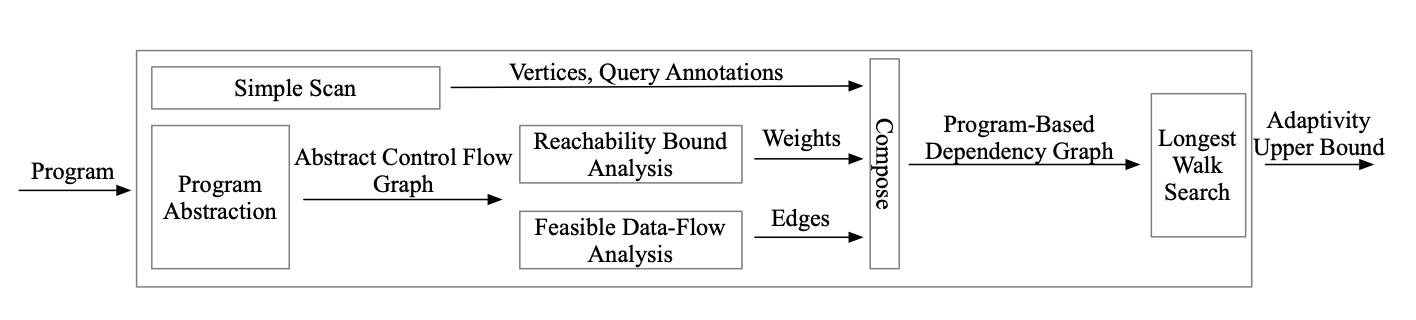
\includegraphics[width=\textwidth]{adapfun}
%   \caption{Seattle Mariners at Spring Training, 2010.}
%   \Description{Enjoying the baseball game from the third-base
%   seats. Ichiro Suzuki preparing to bat.}
%   \label{fig:teaser}
% \end{teaserfigure}

\received{20 February 2007}
\received[revised]{12 March 2009}
\received[accepted]{5 June 2009}

%%
%% This command processes the author and affiliation and title
%% information and builds the first part of the formatted document.
\maketitle

%%%%%%%%%%%%%%%%%%%%%%%%%%%%%%%%%%%%%%%%%%% Introduction and Overview %%%%%%%%%%%%%%%%%%%%%%%%%%%%%%%%%%%%%%%%%%% 

\section{Introduction}
\label{sec:intro}

Gulwani et. al~\cite{GulwaniZ10} first introduced \emph{reachability-bound analysis} as a way to provide upper bounds on the number of times a given program location 
is visited during program execution.
Obtaining tight reachability-bounds is useful in many applications.
For example from a privacy and security perspective,
how much secret information is leaked by a program may depend on the number of times a certain operation that leaks the data
is executed~\cite{Malacaria07};
from an efficiency perspective, when different program locations consume different resources, a precise reachability-bound for each location can help to estimate the resource cost more accurately than just computing the overall complexity.

%Existing works all have different limitations when inferring the \emph{reachability-bound}.
Gulwani et. al~\cite{GulwaniZ10}
give a two-step solution combining program abstraction with a set of proof-rules that are used to compute the actual reachability-bounds. This combination is effective at computing reachability-bounds for a rich class of programs, however, it also has limitations. This method 
computes complexity bounds for loops and over-approximate the reachability-bounds of the different locations inside the loop by using this bound. This result in an over-approximation of the reachability-bounds of several locations, especially when there are loops with multiple paths.

A similar approach to reachability-bounds can be also computed, in principle, using techniques from \emph{amortized program complexity analysis}~\cite{BradleyMS05,CookSZ13,Zuleger18,ZulegerGSV11,SinnZV14,SinnZV17,LuCT21,AliasDFG10}. Indeed, using techniques like ranking functions,  counter increments, difference constraints, etc.
one can estimate 
precise bounds on loop iterations and execution time, and in turn obtain reachability bounds for complex programs. However, these techniques are designed to capture the worst-case or overall complexity, and again they may over-approximate the reachability-bounds of certain locations. This is again particularly evident when a loop contains multiple paths, since in this situation one usually obtains an overall complexity bound which is greater than the reachability-bounds on some locations of some of the paths. 

To overcome these limitations, 
we introduce a new path-sensitive reachability-bound analysis that combines ideas from amortized complexity analysis with ideas from 
\emph{path refinement complexity analysis}~\cite{GustafssonEL05,ManoliosV06,BalakrishnanSIG09,SharmaDDA11,Flores-MontoyaH14,HumenbergerJK18,CyphertBKR19,GulwaniJK09,ZulegerGSV11}.
% can help to summarize the loop paths and compute the program complexity path-sensitively. However, they still do not compute the  reachability-bound for every program location.
Specifically, we propose a new algorithm which is built over a program abstract transition graph, and by combining amortized  analysis with loop summarization-based multipath refinement mitigates the limitations faced by either technique individually. 
% \end{itemize}
%

More in details, our algorithm first uses the difference constraints program abstraction model~\cite{SinnZV17,SinnZV14} enriched with boolean expressions to generate an abstract transition graph.
 %in Section~\ref{sec:progabs}
Then the algorithm performs both path refinement and amortized complexity analysis through ranking estimation over this graph.
%in Section~\ref{sec:refine} and  Section~\ref{sec:rank}.
By computing the ranking function, we effectively alternate computation for the loop bound with the bound invariant of the ranking function. 
% $\locbound(\absevent, c)$ for each transition edge $\absevent$, 
% and estimating its bound invariant in Section~\ref{sec:rank}.
We also leverage the path-insensitivity of ranking function estimation through a lightweight path refinement algorithm adopted from~\cite{GulwaniJK09}.
Building on this combination, we then focus on two useful quantities which we call \emph{path reachability-bound} and \emph{loop reachability-bound}.
The first one bounds the evaluation times of each loop-free and interleave-free path in a refined program, and the second one bounds the iterations of an outer loop w.r.t. the inner loop such that in these iterations of the outer loop, the inner loop is ``entered''. 
We present algorithms for estimating these two quantities and using them we can then 
%Section~\ref{sec:looprb} and~\ref{sec:pathrb} 
compute the \emph{reachability-bound} for each program point in a path-sensitive way.
%in Section~\ref{sec:psrb}.
We have implemented our algorithm in a prototype and evaluated it on 290 program extracted from different benchmarks. Our evaluation %Section~\ref{sec:eval} 
shows that we can accurately estimate different bounds for different locations in programs with loops containing multiple paths. Based on this, we can also compute a tighter overall complexity compared to the state-of-art worst-case complexity analysis tools.

To summarize, our contributions are as follows.
\\
% \begin{itemize}
% \item 
1. We introduce a path-sensitive reachability-bound algorithm 
combining \emph{amortized bound analysis}  and \emph{path refinement}. The algorithm computes tight bounds on the times that each program point is evaluated.
\\
% \item 
% 2. The combination of \emph{amortized bound analysis} through ranking function estimation and the path refinement approach in our algorithm.
% % \item 
% \\
2. We identify two quantities,  \emph{path reachability-bound} and \emph{loop reachability-bound}, which are useful to measure precise information about the program execution.  We also propose two algorithms for soundly estimating these two quantities.
% \item 
\\
3. We develop a prototype implementation with evaluation over 290 programs.
 The evaluation shows improvement in precision compared to other tools for reachability-bound analysis and the worst-case complexity analysis.
% \end{itemize}

\section{Related Work.}
% \begin{itemize}
% \item 
\emph{Program Abstraction.}
Program abstraction is commonly used in program analysis as a preprocessing step to abstract program features and generates transition graphs or systems. For example, Gulwani et. al~\cite{GulwaniZ10} summarizes programs into some underlying abstract domains (the unified lattice~\cite{CousotH78}, polyhedra~\cite{CousotC77} or octagonal~\cite{Mine06})
and generates transition systems for loop counters.
\cite{KincaidCBR18} abstracts the program into the wedge domain and computes the non-linear loop invariant.
% While it only works well for the specific targeting problem.
Efficiency is the main bottleneck when generating and solving the constraint.
We choose to use the difference constraint-based program abstraction model~\cite{SinnZV17,SinnZV14} combined with boolean expressions to generate our abstract transition graph.
It is more accurate in the sense of representing the program loops path-sensitively. This representation is also comparatively lightweight.

% \item 
\emph{Amortized Complexity Analysis.}
This line of complexity analysis follows the idea of the
% \emph{amortized complexity analysis}
% originated 
from Tarjan's influential paper~\cite{PotechinP17}. It is usually combined with ranking functions~\cite{BradleyMS05,CookSZ13,Zuleger18} or counter increments~\cite{ZulegerGSV11,SinnZV14,SinnZV17,LuCT21,AliasDFG10}.
% They do well in nested loops by alternating the loop bound computation with the ranking or counter estimation. This alternation is efficient without recursively unrolling the nested loops when composing the bound of different paths.
 % \\
 But estimating the counter or ranking function invariant ignores the interleaving between multiple paths in the same loop,
% Most of them 
such as the tools CofloCo~\cite{Montoya17,Flores-MontoyaH14,Flores-Montoya16}, KoAT~\cite{BrockschmidtEFFG16,BrockschmidtEFFG14,FalkeKS12,FalkeKS11}, the algorithm in~\cite{LuCT21}, and etc.
% over-approximate the loop bound when the path interleaving affects loop execution.
It is hard to repurpose their result as the reachability-bound on different points.
% loop bound path-insensitively as the reachability-bound on different points.
Another kind of \emph{amortized complexity analysis} based on type refinement or annotation~\cite{CraryW00,JostHLH10,CicekBG0H17,RajaniG0021,CarbonneauxHS15} has the same weakness in the multipath loops, resulting in the over-approximation of the resource cost on different program points.
We choose to use difference-constraints based approach and enrich it with boolean expressions and path-sensitivity according to the Alg.~2 in~\cite{SinnZV14},
% which assigns a variable to each edge on which this variable decrease as its ranking function.
the Alg.~3 in~\cite{ZulegerGSV11},
and the Def.~25 in Section 4 from~\cite{SinnZV17}.

\emph{Path Refinement Based Complexity Analysis}.
Another line of loop bound analysis through loop summarization and path refinement seeks precise loop path representation~\cite{ManoliosV06,BalakrishnanSIG09,SharmaDDA11,Flores-MontoyaH14,HumenbergerJK18,CyphertBKR19}, and explicating the interleaving between paths~\cite{GulwaniJK09,ZulegerGSV11}.
\cite{KincaidBCR19,KincaidCBR18,BreckCKR20} introduce some loop summarization techniques which can help to improve the accuracy of the path refinement but specifically for non-linear loops, program recurrence, etc.
% summarization techniques~\cite{KincaidCBR18} and the invariant generating algorithm considering recurrence in~\cite{BreckCKR20}. 
However, when composing the bound between nested loops, recursively unrolling the nested loops is heavy and non-terminating in most cases.
%
Our method simplifies the path refinement algorithm in~\cite{GulwaniJK09} using contextualization techniques based on~\cite{ZulegerGSV11,SinnZV14,ManoliosV06}.
We also limit the iterations of the refinement algorithm to a constant in our bound analysis algorithm.
% %


\section{Technique Challenges and Algorithm Overview}
\label{sec:overview}
% Plan:
% \textbf{Two Examples + Algorithm Overview}
% \begin{itemize}
% \item {Multiple-Path While Loop}
% \\
% \textbf{The First Challenge/Problem from The Example, 
% and the Overview of the New Techniques Targeting This Problem}
% \item {Nested While Loop}
% \\
% \textbf{The Second Challenge/Problem from The Example,
% and the Overview of the New Techniques Targeting This Problem}
% \end{itemize}
In this section, we discuss two representative examples with
challenges of analyzing the symbolic
\emph{reachability-bound} on
every control location.
We also give the technique overview of our algorithm.
%
\subsection{Multiple-Path Loop}
\label{sec:overview-multiplepath}
    { \footnotesize
    \begin{figure}
    \centering
    %
    \begin{subfigure}{.27\textwidth}
        $
        \begin{array}{l}
          \kw{twoPathsWhile}(n, m) \triangleq \\
        \clabel{ \assign{i}{n} }^{0} ;
        \clabel{ \assign{j}{0} }^{1} ; \\
        L_2:    \ewhile ~ \clabel{i > 0}^{2} ~ \edo ~ \\
            \qquad \big(
              \eif(\clabel{j < m}^{3}, \\
              \qquad \ethen  \clabel{\assign{j}{j + 1}}^{4}; \\
              \qquad \qquad \clabel{\assign{i}{i - 1}}^{5},\\
              \qquad \eelse \clabel{\assign{j}{0}}^{6});
              \big)
            \end{array}
            $
\vspace{-0.2cm}
\caption{}
\end{subfigure}
\begin{subfigure}{.71\textwidth}
\begin{subfigure}{.67\textwidth}
\begin{centering}
\begin{tikzpicture}[scale=\textwidth/20cm,samples=200]
    \draw[] (-8, 10) circle (0pt) node{{ $0$}};
    \draw[] (-4, 10) circle (0pt) node{{ $1$}};
    \draw[] (0, 10) circle (0pt) node{{ $2$}};
    \draw[] (0, 7) circle (0pt) node{{$3$}};
    \draw[] (-3, 4) circle (0pt) node{{ $4$}};
    \draw[] (-8, 4) circle (0pt) node{{ $5$}};
    \draw[] (4, 4) circle (0pt) node{{ $6$}};
    % Counter Variables
    \draw[] (5, 10) circle (0pt) node {\textbf{$\lex$}};
    %
    % Control Flow Edges:
    \draw[ thick, -latex] (-7, 10)  -- node [above] {$i' \leq n$}(-4.5, 10);
    \draw[ thick, -latex] (-3, 10)  -- node [above] {$j' \leq 0$}(-0.5, 10);
    \draw[ thick, -latex] (0, 9.5)  -- node [left] {$i > 0$} (0, 7.5) ;
    \draw[ thick, -latex] (0.5, 7)  -- node [below] {$ j \geq m $}  (4, 4.5);
    \draw[ thick, -latex] (-7.5, 4.5)  to  [out=90,in=180]  node [left] {$i' \leq i - 1$ }(-0.5, 9.5);
    \draw[ thick, -latex] (4.5, 4)  to  [out=70,in=0]   node [right] {$j' \leq 0 $}(0.5, 9.5);
    \draw[ thick, -latex]  (-0.5, 7) -- node  {$j < m$}  (-3, 4.5) ;
    \draw[ thick, -latex]  (-3.5, 4) -- node [above] {$j' \leq j + 1$}  (-7, 4) ;
    \draw[ thick, -latex] (0.5, 10)  -- node [above] {$i \leq 0$}  (4.5, 10);
  \end{tikzpicture}
        \caption{}
\end{centering}
\end{subfigure}
{\small
\begin{subfigure}{.3\textwidth}
\begin{centering}
        $\tpath_0 = 0 \to 1 \to 2$ \\
        $\tpath_2 = 2 \to 3 \to 6 \to 2$ \\ 
        $\tpath_1 = 2 \to 3 \to 4 \to 5 \to 2$ \\
        $\tpath_3 = 2 \to \lex$
        \caption{}
\end{centering}
\end{subfigure}
}
{\small
\begin{subfigure}{.8\textwidth}
\begin{centering}
    $
    \tpath_0 ; 
    \rpchoose{2: \rprepeat(\rprepeat(\tpath_1); \tpath_2), 
    2: \rprepeat(\tpath_1)}; \tpath_3.
    $
\end{centering}
\end{subfigure}
}
\end{subfigure}
\vspace{-0.2cm}
\caption{
    (a) The two paths loop example,
    (b) the Abstract Transition Graph for $\kw{twoPathsWhile}(n, m)$,
    (c) the Simple Transition Paths of $\kw{twoPathsWhile}(n, m)$.}
    \vspace{-0.5cm}
        \label{fig:whileTwoCounters-overview}
    \end{figure}
    }



Figure~\ref{fig:whileTwoCounters-overview}(a) shows an example of a two paths loops
with different \emph{reachability-bounds} on the control locations in different paths.
This example is adopted from the example in~\cite{Sumit2010rechability}, which
is a skeleton code from the .Net base-class library.
\\
In this example, given $n \geq m$,
the precise \emph{reachability-bound}s for control locations $4$ and $5$ are both $m \times \lfloor\frac{n}{m}\rfloor$,
for location $2$ and $3$ are $(m + 1) \times \lfloor\frac{n}{m}\rfloor + 1$, 
and $1$ for locations $0, 1$ and $\lex$. 
\highlight{Notice here, though within the same loop $L_2$, the bounds for locations $4$ and $5$ on the first branch, and $6$ on the second branch are different.}
% \\
% In order to know that the locations in first branch ($4$ and $5$) are reached at most $m \times \lfloor\frac{n}{m}\rfloor$ times
% while $6$ in second branch $\lfloor\frac{n}{m}\rfloor$ times
%  during program execution,
% we need to know that the two if branches are interleaved and executed alternatively after each other
% during the iterations of the enclosed loop.
\\
However, the state-of-art \emph{reachability-bound} analysis~\cite{Sumit2010rechability}
gives the same \emph{reachability-bound}, $n + \lfloor\frac{n}{m}\rfloor$ for all the locations within the loop $L_2$, which is tight w.r.t. $L_2$'s iteration times but not for different locations inside $L_2$ without considering multiple paths.
Among works on program complexity, cost and loop bound analysis, \cite{GulwaniJK09} can also compute the tight bound on the loop iteration but not reachability-bound on each location path-sensitively.
Though we can use it as the \emph{reachability-bound} for location $1$ and $2$,
the \emph{reachability-bounds} for control locations $4, 5$ and $6$ are still unclear.
\paragraph{Path Reachability-bound}
To compute the bounds for locations on different paths of a loop, we compute the \emph{path reachability-bound},
which is the first key idea of this path-sensitive \emph{reachability-bound} analysis algorithm. This bound approximate the evaluation times of each loop free path instead of the entire multipath loop.
\\
% Our algorithm combines the idea of \emph{difference constraint} based program complexity analysis method from \cite{sinn2017complexity}
% and the control-flow refinement technique from~\cite{GulwaniJK09}.
For this example, we first
generate the abstract transition graph for the program using the difference constraints, such as Figure~\ref{fig:whileTwoCounters-overview}(b).
Then it transforms every the loop in $\kw{twoPathsWhile}$ using the control-flow refinement technique from~\cite{GulwaniJK09} and generates a refined program $\rprog$ as
\\
% 
% The refined program for program $\kw{twoPathsWhile}$ is
% \[
  $
  \tpath_0 ; 
  \rpchoose{2: \rprepeat_2(\rprepeat_1(\tpath_1); \tpath_2), 
  2: \rprepeat_1(\tpath_1)}; \tpath_3.
  $
% \]
\\
Each $\tpath_i$ in this refined program is a \emph{simple transition path} we computed in a pre-procedure, which is loop free and not interleave with the other $\tpath_j, j \neq i$ as in Figure~\ref{fig:whileTwoCounters-overview}(c).
% Every path will not interleave with the others. 
Then we compute the \emph{path reachability-bound} for every $\tpath_i$,
$\inoutB(\rprog, \tpath_i)$ during the execution of $\rprog$.
% which is a bound on the reachability time of $\tpath$ during the execution of $\rprog$.
The \emph{path reachability-bound}s for the four simple transition paths in this example are
$\inoutB(\rprog, \tpath_1) = \max\{m, m \times \lfloor\frac{n}{m}\rfloor\}$,
$\inoutB(\rprog, \tpath_2) = \lfloor\frac{n}{m}\rfloor$,
and $\inoutB(\rprog, \tpath_0) = \inoutB(\rprog, \tpath_3) = 1$.
% \\
% Then we use this bounds
% and another \emph{loop reachability-bound}
% to compute the final \emph{reachability-bound} for each location.
Since there isn't nested loop in this example, we simply sum up $\inoutB(\rprog, \tpath)$ over the $\tpath$ where a certain location shows up
and as the \emph{reachability-bound} of this location.
Then we get the precise \emph{reachability-bound} for every location in program $\kw{twoPathsWhile}$ as
$\psRB(0) = \psRB(1) = \psRB(\lex) = 1$,
$\psRB(4) = \psRB(5) = \max\{m, m \times \lfloor\frac{n}{m}\rfloor\}$,
$\psRB(3) = \psRB(2) = \max\{m, m \times \lfloor\frac{n}{m}\rfloor\} + \lfloor\frac{n}{m}\rfloor + 1 $,
and $\psRB(6) = \lfloor\frac{n}{m}\rfloor$.
%
\subsection{Nested Loops with Related Iterator}
\label{sec:overview-nestedwhile}
However, when there exists nested loop, computing the \emph{reachability-bound} for each location encounters another challenge.
The \emph{path reachability-bound} is precise for each path w.r.t. the innermost loop but not the outer nested loops.
Figure~\ref{fig:threeWhile-overview}(a) shows an example of the nested loops with related 
iterators.
This example is adopted from the example in~\cite{GulwaniJK09}, which is common in product code.
\\
In line 8, $i$ is reset by $w$ and $w$ is reset by $j$ at line 5. So the
while $L_6$ is only executed in the first iteration of while loop $L_1$ and $L_3$.
% \\
The while loop $L_3$ at line 3 is executed only in 
the first $m - N$ iterations of the 
$L_1$ because $j$ is reset by $i$ in line 2.
% \\
So the total iterations of all the three loops is
$n + m^2 - m \times N$,
and the precise \emph{reachability-bound} for location $7$ inside the $L_6$ is $N$,
for locations $4, 5$ and $8$ between the $L_3$ and $L_6$ are $(n-N) \times (m - N)$,
and $n - N$ for locations $2$ and $9$.
% \\
\highlight{Notice here the \emph{reachability-bounds} for the locations inside the loop $L_6$ is 
the same as its loop iteration bound, as well as our \emph{path reachability-bound}.
However, for the locations between $L_3$ and $L_6$,
the \emph{reachability-bounds} are the multiplication of the inner and outer loop iteration bounds.}
\\
To the best of our knowledge, the loop bound analysis method in \cite{GulwaniJK09} can only give a loose bound $n + (m \times n) + N$ for the entire loop complexity, and 
the DC-based algorithm in \cite{sinn2017complexity} is able to
compute a better but still loose bound, $n + m^2 - m \times N$ on total iteration times.
None of them can give the precise \emph{reachability-bound} for every location in these nested loops,
which is non-trivial to compute even though knowing the loop bound,
especially for the locations similar to $7$ in $\kw{threeNestedWhile}$.
\\
\highlight{
In order to precisely compute how many times the location $7$ is reached, we need to know
the numbers of iterations of the outside loop $L_3$ and $L_1$ such that,
during these iterations, the loop $L_6$ is ``entered''. 
We call this the \emph{loop reachability} of the location within loop $L_6$ w.r.t the loops $L_3$ and $L_1$.
Then by multiplying the loop iteration bound of the $L_6$ with its \emph{loop reachability} times w.r.t the  $L_3$ and $L_1$, we can compute the precise
\emph{reachability-bounds} for location $7$.
}
\\
\highlight{
This quantity isn't considered or computed in any of the previous works.
The \emph{Progress Invariant} method in \cite{GulwaniJK09} is only able to compute
the
bound on iteration numbers
of the inner loop $L_6$ in each iteration of $L_3$ and $L_1$, which are both $N$.
So they have to over-approximate the reachability-bound for locations inside $L_6$ with the
overall program complexity, i.e., $n + m^2 - m \times N$.
% \\
For the same reason, the DC-based algorithm in \cite{sinn2017complexity}
is only able to
compute the precise combined loop bound and the local bound of each loop
separately as well.
% We are still unable to know the precise \emph{reachability-bound} for the locations in the innermost loop.
}
\paragraph*{Loop reachability-bound.}
In this sense, this \emph{loop reachability-bound}, $\lpchB(L:\rprog, \tpath)$ is our second key idea.
For each transition path $\tpath$ w.r.t each of the loops $L:\rprog$ in which $\tpath$ is nested,
$\lpchB(L:\rprog, \tpath)$ 
\highlight{is a bound on the iterations for
the outside loop, $L:\rprog$ w.r.t. the innermost loop where $\tpath$ is enclosed,
such that during these iterations of $L:\rprog$, the innermost loop is ``entered''. 
This is distinguished from the traditional methods, which only estimate the bound on the inner loop's iteration number
in one iteration of the outside loop.}
\\
Similar to the $\kw{twoPathsWhile}$ example, we also generate its abstract transition graph as well in Figure~\ref{fig:threeWhile-overview}(a),
and compute its refined program,
$\rprog = \tpath_0; 1: \rprepeat(\tpath_1;$ 
$3: {\rprepeat(\tpath_2; 6 : {\rprepeat(\tpath_3)}; \tpath_4)}; \tpath_5);$ 
$\tpath_6$,
where the $\tpath_0, \ldots$ are shown in the middle part of Figure~\ref{fig:threeWhile-overview}(b).
We use $\rprog_1$ and $\rprog_3$ denote the body of the loop $L_1$ and $L_3$ respectively as in the bottom part of Figure~\ref{fig:threeWhile-overview}(b).
% to denote ${\rprepeat(\tpath_1; 3: {\rprepeat(\tpath_2; 6 : {\rprepeat(\tpath_3)}; \tpath_4)}; \tpath_5)}$
% and $\rprog_3 = {\rprepeat(\tpath_2; 6 : {\rprepeat(\tpath_3)}; \tpath_4)}$
In the first step, we still compute the \emph{path reachability-bound} for each $\tpath_i$ but only w.r.t. the closest loop it is nested.
Then differently from $\kw{twoPathsWhile}$,
we compute \emph{loop reachability-bound} for each $\tpath_i$ w.r.t. each of its nested loops.
For example, for $\tpath_3$ we compute
$\lpchB(1: \rprog_1, \tpath_3) = 1$ and
$\lpchB(3: \rprog_3, \tpath_3) = 1$.
Both are tight because loop $L_6$ will only be entered once among all iterations of $L_1$ and $L_3$, and in all the rest iterations, the body of loop $L_6$ isn't executed at all.
So $1$ as \emph{loop reachability-bound} of this path is tight w.r.t. both the loop $L_3$ and $L_1$.
% In the same way, we also compute $\lpchB(3: \rprog_3, \tpath_3) = 1$ precisely.
Then for each $\tpath_i$, the multiplication of its \emph{path reachability-bound} with all its \emph{loop reachability-bound}s is an accurate \emph{loop reachability-bound} for the locations on this path.
By summing up the reachability-bound of the path where each location shows up,
% as its \emph{reachability-bound} as before.
% and multiply this result by all its \emph{loop reachability-bound}s.
% In this way, 
we compute $N$ as the \emph{reachability-bound} of location $7$, which is tight.
    %
    \begin{figure}
    \centering
    %
    \vspace{-0.8cm}
    \begin{subfigure}{.45\textwidth}
        $
        \begin{array}{l}
            N < m < n\\
            \kw{threeNestedWhile}(n, m, N) \triangleq \\
            \clabel{ \assign{i}{0} }^{0} ; \\
                L_1: \ewhile ~ \clabel{i < n}^{1} ~ \edo ~ \\
                \quad (
                 \highlight{\clabel{\assign{j}{0}}^{2}} ;\\
                 L_3:  \quad \ewhile ~ \clabel{j < m}^{3} ~ \edo ~ \\
                \quad \quad ( \clabel{\assign{j}{j+1}}^{4};\\
                  \quad \quad \highlight{\clabel{\assign{w}{i}}^{5}};\\
                  L_6:  \quad \quad \ewhile ~ \clabel{w < N}^{6} ~ \edo ~ \\
                  \quad \quad \quad ( \clabel{\assign{w}{w + 1}}^{7} ); \\
                      \quad \quad \clabel{\assign{i}{w}}^{8}
                      ); \\
                      \quad \clabel{\assign{i}{i+1}}^{9})
            \end{array}
            $
            \vspace{-0.2cm}
            \caption{}
        \end{subfigure}
    \begin{subfigure}{.48\textwidth}
        \begin{centering}
            \begin{tikzpicture}[scale=\textwidth/20cm,samples=200]
                \draw[] (-5, 10) circle (0pt) node{{ $0$}};
                \draw[] (0, 10) circle (0pt) node{{ $1$}};
                \draw[] (6, 10) circle (0pt) node {{$\lex$}};
                \draw[] (0, 7) circle (0pt) node{{$2$}};
                \draw[] (0, 4) circle (0pt) node{{ $3$}};
                \draw[] (-5, 4) circle (0pt) node{{ $9$}};
                \draw[] (0, 1) circle (0pt) node{{ $4$}};
                \draw[] (4, 1) circle (0pt) node{{ $5$}};
                \draw[] (8, 1) circle (0pt) node{{ $6$}};
                \draw[] (13, 1) circle (0pt) node{{ $7$}};
                \draw[] (5, 6) circle (0pt) node{{ $8$}};
                % Counter Variables
                %
                % Control Flow Edges:
                \draw[ thick, -latex] (-4, 10)  -- node [above] {$i \leq 0$}(-0.5, 10);
                \draw[ thick, -latex] (0, 9.5)  -- node [left] {$i < k$} (0, 7.5) ;
                \draw[ thick, -latex] (0, 6.5)  -- node [right] {$j \leq m$} (0, 4.5) ;
                \draw[ thick, -latex] (0, 3.5)  -- node [left] {$j > 0$} (0, 1.5) ;
                \draw[ thick, -latex] (-0.5, 4)  -- node [above] {$j \leq 0$} (-4.5, 4) ;
                \draw[ thick, -latex] (-4.5, 4.5)  to  [out=90,in=180]  node [left] {$i \leq i + 1$ }(-0.5, 9.5);
                \draw[ thick, -latex] (0.5, 10)  -- node [above] {$i \leq 0$}  (5.5, 10);
                \draw[ thick, -latex] (0.5, 1)  -- node [above] {{\footnotesize $j \leq j - 1$}}  (3.5, 1);
                \draw[ thick, -latex] (4.5, 1)  -- node [above] {$w \leq i$}  (7.5, 1);
                \draw[ thick, -latex] (8.5, 1)  -- node [above] {{\footnotesize $w < N$}}  (12.5, 1);
                \draw[ thick, -latex] (8, 1.5)  to [out=90,in=0] node [left] {{$w \geq N$}}  (5.5, 6);
                \draw[ thick, -latex] (13, 1.5)  to  [out=120,in=60] node [above] {$w \leq w + 1$}  (8, 1.5);
                \draw[ thick, -latex] (5, 6.5)  to  [out=120,in=0]  node [right] {$i \leq i - 1$ }(0.5, 9.5);
                \end{tikzpicture}
%     \caption{}
%     \end{centering}
%     \end{subfigure}
% \begin{subfigure}{.2\textwidth}    
% \begin{centering}
    {\small
$
    \begin{array}{ll}
        \tpath_0 = (0 \to 1)
        &
        \tpath_4 = (6 \to 8 \to 3)
        \\        
        \tpath_1 = (1 \to 2 \to 3)
        &
        \tpath_5 = (3 \to 9 \to 1)
        \\
        \tpath_2 = (3 \to 4 \to 5 \to 6)
        &
        \tpath_6 = (1 \to \lex)
        \\
        \tpath_3 = (6 \to 7 \to 6)
    \end{array}
$
}
\vspace{-0.2cm}
\caption{}
\end{centering}
\end{subfigure}
% $
%     \begin{array}{l}
%         \rprog_1 = {\rprepeat(\tpath_1; 3: {\rprepeat(\tpath_2; 6 : {\rprepeat(\tpath_3)}; \tpath_4)}; \tpath_5)}
%         \\
%         \rprog_3 = {\rprepeat(\tpath_2; 6 : {\rprepeat(\tpath_3)}; \tpath_4)}
%     \end{array}
% $
$\rprog = \tpath_0; 1: \rprepeat(\tpath_1; 3: {\rprepeat(\tpath_2; 6 : {\rprepeat(\tpath_3)}; \tpath_4)}; \tpath_5);\tpath_6$
\vspace{-0.2cm}
\caption{
    (a) An example of three nested loops with related iterators,
    (b) the abstract transition graph, simple transition paths and loop body.}
    \vspace{-0.8cm}
        \label{fig:threeWhile-overview}
    \end{figure}

\highlight{
\textbf{Step 1: }
The Section~\ref{sec:progabs} first 
computes the \emph{Abstract Transition Graph} as in Figure~\ref{fig:relatedNestedWhileOdd-overview}(b).
Each edge $l \xrightarrow{dc} l'$ is an abstract transition $\absevent = (l, dc, l')$ annotated with a constraint $dc$ corresponding to the command of label $l$.

% \textbf{Step 2: Program Refinement}
\textbf{Step 2: }
The second step in Section~\ref{sec:refine}
computes the \emph{Refined Program}, $\rprog$ for a program $c$ based on 
its abstraction transition graph and transforms the multiple-paths loops
into multiple loops where
the interleaving of paths is explicit as in bottom part of Figure~\ref{fig:relatedNestedWhileOdd-overview}(c).
It has two interleaving patterns in the loop $L_1$.
%  denoted as $\rprog_1^1$ and $\rprog_1^2$.

% \textbf{Step 3: Ranking Function Estimation}
\textbf{Step 3: }
In the meanwhile, Section~\ref{sec:rank} computes the \emph{Ranking Function}, $\locbound(\absevent, c)$ 
for every edge $\absevent$ 
and estimates an upper bound invariant for each.

% \textbf{Step 4: Path-sensitive Reachability-bound Computation.}
\textbf{Step 4: }
% The \emph{path-sensitive reachability-bound} 
The algorithm computes the \emph{Reachability-bound}, $\psRB(l, c)$ for every program point $l$ using the $\rprog$ and the upper bound invariant of the $\locbound(\absevent, c)$ where $\absevent = (l,dc,l')$.
It requires to compute our two novel quantities, the \emph{Path Reachability-bound}, $\inoutB(\rprog, \tpath, c)$ and the \emph{Loop Reachability-bound}, $\lpchB(l: \rprog, \tpath, c)$.
Section~\ref{sec:psrb} introduces this algorithm and the following sections describe the computations. 
The soundness of each algorithm is in the Appendices and the input $c$ will be omitted if the context is clear.

In the first interleaving pattern, $\rprog_1^1 = 1: \rprepeat(\tpath_1; 4:\rprepeat(\tpath_3); \tpath_2; \tpath_4)$ in Figure~\ref{fig:relatedNestedWhileOdd-overview},
we first compute $\outinB(4:\rprepeat(\tpath_3), \tpath_3) = n - m$
 for $\tpath_3$ in its innermost loop $L_4$ as a local \emph{path reachability-bound} by Section~\ref{sec:pathlocalrb}.
Then we compute $\lpchB(\rprog_1^1, \tpath_3) = 1$ w.r.t. its outer loop $L_1$ in Section~\ref{sec:looprb}. In the second interleaving pattern, we compute $\outinB(4:\rprepeat(\tpath_3), \tpath) = n - m - 3$ and the same for $\lpchB$.
So Section~\ref{sec:pathrb} computes $\inoutB(\rprog, \tpath_3) = \max\{ 1 \times (n - m), 1 \times (n - m - 3) \} = n - m$ globally.

Then for every program point $l$, we sum up all the $\inoutB(\rprog, \tpath)$ over $\tpath$ that contains $l$ and get $\psRB(l, c)$.
Since point $5$ only shows up on $\tpath_3$, we compute \highlight{$\psRB(5, c) = n - m$}.
The points $0$ and $\lex$ are not in any loop, so $\psRB(0) = \psRB(\lex) = 1$,
The points $3, 6, 7$ and $8$ which only show up once on $\tpath_2$ and $\tpath_4$ are all equal to $\lfloor\frac{m}{4}\rfloor$, which are same as their $\inoutB$.
For the loop headers $1$ and $4$, we only sum up the $\inoutB(\rprog, \tpath)$ where they show up as start-point of the $\tpath$.
So $\psRB(4) =  \lfloor\frac{m}{4}\rfloor + n - m + 1$ and $\psRB(1) = 2 \times \lfloor\frac{m}{4}\rfloor + 1$ all as expected.
% For the other points in different branches and loop, we compute
% $\psRB(1) =2 \times \lfloor\frac{m}{4}\rfloor + 1$,
% $\psRB(2) =2 \times \lfloor\frac{m}{4}\rfloor $, 
% $\psRB(3) = \psRB(6) = \psRB(7)  = \psRB(8) = \lfloor\frac{m}{4}\rfloor $,
% \highlight{$\psRB(5) = \lfloor\frac{m}{4}\rfloor \times 1$},
% and $\psRB(4) =  \lfloor\frac{m}{4}\rfloor + n - m + 1$ as expected.


%     % Our static program analysis algorithm computes 
% % a \emph{reachability-bound} for every program point $l$ in a program $c$ in a path sensitive manner.
% % The main steps of this algorithm and the organization the following sections are summarized as follows.
% \begin{enumerate}
%     \item  The Section~\ref{sec:progabs} first 
%     computes the \emph{Abstract Transition Graph}, $\absG(\kw{nestedOdd})$ as in Figure~\ref{fig:relatedNestedWhileOdd-overview}(b).
%     Each edge $l \xrightarrow{dc} l'$ is an abstract transition with annotated with a constraint corresponding to the command of label $l$.
%     \item The second step in Section~\ref{sec:refine}
%     computes the \emph{Refined Program}, $\rprog$ for a program $c$ based on 
%     its abstraction transition graph and transforms the multiple-paths loops
%     into multiple loops where
%     the interleaving of paths is explicit as in bottom part of Figure~\ref{fig:relatedNestedWhileOdd-overview}(c).
%     \item In the same time of refining the program, we also compute the \emph{Ranking Function} in Section~\ref{sec:rank}
%     for every edge 
%     and estimate the upper bound invariant w.r.t, the input variables on every ranking function's maximum value.
%     \item The \emph{path-sensitive reachability-bound} algorithm computes the \emph{reachability-bound}, $\psRB(l, c)$ for every program point.
%     It relies on the \emph{Refined Program} and the upper bound invariant of the \emph{Ranking Function} computed previously.
%     It requires to compute our two novel quantities, the \emph{Path Reachability-bound}, $\outinB(\rprog, \tpath)$ and the \emph{Loop Reachability-bound}, $\lpchB(l: \rprog, \tpath)$.

%     For the transition path $\tpath_3 = 4 \to 5 \to 4$ in the first interleaving pattern where $\rprog_1^1 = 1: \rprepeat(\tpath_1; 4:\rprepeat(\tpath_3); \tpath_2; \tpath_4)$,
%     we compute $\outinB(4:\rprepeat(\tpath_3), \tpath) = m$ w.r.t its innermost loop $L_4$ as a local \emph{Path Reachability-bound} in Section~\ref{sec:pathlocalrb}
%     We also compute $\lpchB(\rprog_1^1, \tpath) = 1$ w.r.t. its outer loop $L_1$ in Section~\ref{def:looprb},
%     and Section~\ref{sec:pathrb} computes $\tpath_3$'s global \emph{Path Reachability-bound} $\inoutB(\rprog, \tpath) = m$.

%     By summing up all the \emph{path reachability-bounds}, $\inoutB(\rprog, \tpath)$ over the $\tpath$ which contains the program point $l$, we compute the \emph{Reachability-bound}, $\psRB(l, c)$ for every program point $l \in \lvar(c)$.
%     For the points $0$ and $\lex$ which aren't in any loop, we compute $\psRB(0) = \psRB(\lex) = 1$,
%     For the other points in different branches and loop, we compute $\psRB(1) =2 \times \lfloor\frac{m}{4}\rfloor + 1$,
%     $\psRB(2) =2 \times \lfloor\frac{m}{4}\rfloor $, 
%     $\psRB(3) = \psRB(6) = \psRB(7)  = \psRB(8) = \lfloor\frac{m}{4}\rfloor $,
%     \highlight{$\psRB(5) = \lfloor\frac{m}{4}\rfloor \times 1$},
%     and $\psRB(4) =  \lfloor\frac{m}{4}\rfloor + n - m + 1$ as expected.

%     Section~\ref{sec:psrb} introduces this algorithm and the following sections describe the computations. 
%     % To compute the \emph{reachability-bound}  compute the path reachability-bound for 
%     % We compute the $\lpchB(l: \rprog, \tpath)$ for 
%     % \begin{enumerate}
%         % \item Based on the ranking function and its upper bound invariant, we first compute the \emph{Path Local Reachability-bound}, $\outinB(\rprog, \tpath)$ for every \emph{simple transition path} $\tpath$ in Section~\ref{sec:pathlocalrb}. 
%         % This bounds the reaching / visiting times of $\tpath$ when executing program $\rprog$, and $\rprog$ is the closest loop where $\tpath$ is nested.
%         % The local reachability-bound  considers only the execution of $\tpath$'s closest enclosing loop, i.e., $\kw{enclosed}(\tpath)$.
%         % \item Then in Section~\ref{sec:looprb}, we compute the \emph{Loop Reachability-bound}, $\lpchB(l: \rprog, \tpath)$ for every \emph{simple transition path} $\tpath$
%         % w.r.t its nested loop. 
%         % This is the bound on iteration numbers of the outside loop $l$,
%         % such that during these iterations, the nested loop $l' = \kw{enclosed(\tpath)}$ is executed, i.e., reached.
%         % \item The \emph{Path Reachability-bound}, $\inoutB(\rprog, \tpath)$  is a global upper bound on the execution times of a \emph{simple transition path} $\tpath$ computed in Section~\ref{sec:pathrb}.
%         % With the global reachability-bound of every simple transition path, now we can sum up all the \emph{path reachability-bounds}, $\inoutB(\rprog, \tpath)$ over the $\tpath$ which contains the program point $l$, and compute the \emph{Reachability-bound}, $\psRB(l, c)$ for every program point $l \in \lvar(c)$ as in Definition~\ref{def:point_psrb}.
%     % \end{enumerate}
%     \end{enumerate}
}
% %
\section{Program Model and The Reachability-bound}
\label{sec:preliminary}
% \input{preliminary}
%
%
\subsection{Labeled Language}
\[
\begin{array}{llll}
\mbox{Arithmetic Operators} 
& \oplus_a & ::= & + ~|~ - ~|~ \times 
%
~|~ \div ~|~ \emax ~|~ \emin\\  
% ~|~ \div \\  
\mbox{Boolean Operators} 
& \oplus_b & ::= & \lor ~|~ \land
\\
%
\mbox{Relational Operators} 
& \sim & ::= & < ~|~ \leq ~|~ == 
\\  
%
\mbox{Arithmetic Expression} 
& \aexpr & ::= & 
n ~|~ {x} ~|~ \aexpr \oplus_a \aexpr  
 ~|~ \elog \aexpr  ~|~ \esign \aexpr
\\
%
\mbox{Boolean Expression} & \bexpr & ::= & 
%
\etrue ~|~ \efalse  ~|~ \neg \bexpr
 ~|~ \bexpr \oplus_b \bexpr
%
~|~ \aexpr \sim \aexpr 
\\
%
\mbox{Expression} & \expr & ::= & v ~|~ \aexpr ~|~ \bexpr ~|~ [\expr, \dots, \expr]
\\  
%
\mbox{Value} 
& v & ::= & { n ~|~ \etrue ~|~ \efalse ~|~ [] ~|~ [v, \dots, v]} \\
%
% \\%
\mbox{Label} 
& l & \in & (\mathbb{N} \cup \{\lin, \lex\}) 
% ~|~ (l, n)
\\ 
%
\mbox{Labeled Command} 
& {c} & ::= &  
\clabel{\assign{x}{\expr}}^l 
% ~|~ \clabel{\assign{x}{\query(\qexpr)}}^l
~|~  \clabel{\eskip}^l
~|~ \ewhile \clabel{\bexpr}^{l} \edo {c}
~|~ \eif(\clabel{\bexpr}^{l} , {c}, {c}) 
~|~ {c};{c}  
\\ 
% \\
\mbox{Event} 
& \event & ::= & 
% ~|~ ({x}, l, v, \qval)
({x}, l, v) ~ \mbox{Assignment Event} 
% \\
% &&& 
~|~(\bexpr, l, v) ~ \mbox{Testing Event}
\\
% \mbox{Trace} & \trace
% & ::= & [] ~|~ \event:: \trace ~|~ \trace \tracecat \trace  \\
\mbox{Trace} & \trace
& ::= & [] ~|~ \trace :: \event
\\
\end{array}
\]
% \todo{change trace notation into list, and update corresponding operator nations}
% \\
% \wqside{"$\cdot$" has two meanings? empty, delimit. Trace is list of event?}
We use following notations to represent the set of corresponding terms:
\[
\begin{array}{lll}
\mathcal{VAR} & : & \mbox{Set of Variables}  
% \\ 
% %
% \mathcal{VAL} & : & \mbox{Set of Values} 
% \\ 
% %
% \mathcal{QVAL} & : & \mbox{Set of Query Values} 
\\ 
%
\cdom & : & \mbox{Set of Commands} 
\\ 
%
\eventset  & : & \mbox{Set of Events}  
\\
%
\eventset^{\asn}  & : & \mbox{Set of Assignment Events}  
\\
%
\eventset^{\test}  & : & \mbox{Set of Testing Events}  
\\
%
\ldom  & : & \mbox{Set of Labels}  
\\
% \\
%
{\mathcal{T}} & : & \mbox{Set of Traces}
\\
%
\mathcal{T}_0(c) & : & \mbox{Set of Initial Traces, where all the input variables of the program $c$ are initialized.
}
\end{array}
\]
$FV: \expr \to \mathcal{P}(\mathcal{VAR})$, computes the set of free variables in an expression. To be precise,
$FV(\aexpr)$ and $FV(\bexpr)$
%  and $FV(\qexpr)$ 
represent the set of free variables in arithmetic
expression $\aexpr$ and boolean expression $\bexpr$
%  and query expression $\qexpr$ 
respectively.
%
\subsection{{Trace-based Operational Semantics}}
\label{sec:operational_semantics}
% \subsubsection{Event and Trace}
\paragraph*{Event}
An event tracks useful information about each step of the evaluation, as a quadruple. Its first element is either 
an assigned variable (from an assignment command) or a boolean expression (from the guard of if or while command), follows by 
 the label associated to this event, the value evaluated either from the expression assigned to the variable,
or the boolean expression in the guard.
%
\[
\begin{array}{llll}
  \mbox{Event} 
  & \event & ::= & 
  % ~|~ ({x}, l, v, \qval)
  ({x}, l, v) ~ \mbox{Assignment Event} 
  % \\
  % &&& 
  ~|~(\bexpr, l, v) ~ \mbox{Testing Event}
\end{array}
\]
Event projection operators $\pi_i$ projects the $i$th element from an event: 
\\
$\pi_i : 
\eventset \to \mathcal{VAR}\cup \mbox{Boolean Expression}  \cup \mathbb{N} $
% \subsubsection{Trace}
\paragraph*{Trace}
%
A trace $\trace \in \tdom$ is a list of events, 
collecting the events generated during a specific program execution. 
\[
\begin{array}{llll}
\mbox{Trace} & \trace
& ::= & [] ~|~ \trace :: \event 
% ~|~ []^{\infty}
\end{array}
\]
A trace can be regarded as the program history, 
which records all the evaluations for assignment commands and guards in $\eif$ and $\ewhile$ command.
\\
\highlight{
A trace can be finite ($\trace \in \ftdom$) or infinite $\trace \in \inftdom$.
If a program doesn't terminate when executing under some initial trace,
it produces the infinite trace 
from $\inftdom$, which records a non-terminating computation.
So we denote by $\tdom$ the set of all traces, and $\tdom = \ftdom \cup \inftdom$.
The trace-based semantics with non-terminating execution is defined below following the maximal trace semantics in \cite{Cousot19}.}

We use list notation for traces, where $[]$ is the empty trace, the operator $\traceadd$ combines an event and a trace in a new event, 
and the operator $\tracecat$ concatenates two traces formally defined as follows. 

\begin{defn}[Trace Concatenation, $\tracecat: \tdom \to \tdom\to \tdom $]
  \label{def:trace_concate}
Given two traces $\trace_1 \in \tdom, \trace_2 \in \tdom$, the trace concatenation operator 
$\tracecat$ is defined as:
\[
\trace_1 \tracecat \trace_2 \triangleq
\left\{
\begin{array}{ll} 
  \trace_1 & \trace_2 = [] \lor \trace_1 \in \inftdom \\
  \trace_2 & \trace_1 = [] \lor \trace_2 \in \inftdom \\
  (\trace_1   \tracecat \trace_2'):: \event & \trace_1 \in \ftdom \land \trace_2 = \trace_2' :: \event
  % \trace_2 &  \trace_2 \in \inftdom \\
\end{array}
\right.
\]
\end{defn}

\begin{defn}(An Event Belongs to A Trace)
  An event $\event \in \eventset$ belongs to a trace $\trace \in \tdom$, i.e., $\event \in \trace$ are defined as follows:
%
\begin{equation*}
  \event \in \trace  
  \triangleq \left\{
  \begin{array}{ll} 
    \etrue                  & \trace =  [\event] \tracecat \trace'
     \land \event = \event' \\
    \event \in \trace' & \trace =  [\event'] \tracecat \trace'
      \land \event \neq \event' \\ 
    \efalse                 & \trace = [] \lor \trace \in \inftdom
  \end{array}
  \right.
\end{equation*}
As usual, we denote by $\event \notin \trace$ that the event $\event$ doesn't belong to the trace $\trace$.
\end{defn}
%
In the rest of the paper, we denote by $\bot$ a value s.t. $\bot < n $ for all $n \in \mathbb{N}$.
\begin{defn}[Counter Notation for Program Point]
  \label{def:counter}
The counting operator $\counter : \tdom \to \ldom \to (\mathbb{N} \cup \{\bot, \infty\})$
counts the appearance of a label in a trace.
\[
\begin{array}{llll}
\counter([(x, l, v)] \tracecat \trace', l ) \triangleq \counter(\trace', l) + 1 & \text{if}~ l = l
&
\counter([(b, l, v)] \tracecat \trace', l) \triangleq \counter(\trace', l) + 1 & \text{if}~ l = l
\\
\counter([(x, l', v)] \tracecat \trace', l) \triangleq \counter(\trace', l)   & \text{if}~ l' \neq l
&
\counter([(b, l', v)] \tracecat \trace', l) \triangleq \counter(\trace', l)   & \text{if}~ l' \neq l
\\
\counter({[]}, l) \triangleq 0 & 
&
\counter(\trace, l) \triangleq \bot & \text{if }~ \trace \in \inftdom
\end{array}
\]
{When the input trace is infinite, $\counter(\trace, l)$ returns $\bot$ for any program label $l$.}
\end{defn}
\begin{defn}[Counter Notation for List of Program Point]
  \label{def:lcounter}
  The counting operator $\lcounter : \tdom \to \mathcal{P}(\ldom) \to (\mathbb{N} \cup \{\infty\})$
  counts the appearance of a list of labels $[l_1, \ldots, l_n]$ as follows.
\[
  \begin{array}{ll}
  \lcounter(\trace'' \tracecat \trace', [l_1, \ldots, l_n] ) 
  \triangleq \lcounter(\trace', [l_1, \ldots, l_n]) + 1  & \text{if}~ \pi_2(\trace''[i]) = l_i, \forall i = 1, \ldots, n
  \\ 
  \lcounter([(\_, l, \_)] \tracecat \trace', [l_1, \ldots, l_n] ) 
  \triangleq \lcounter(\trace', [l_1, \ldots, l_n]) & \text{if}~ l \neq l_1
  \\ 
  \lcounter(\trace, [l_1, \ldots, l_n] ) 
  \triangleq \bot & \text{if }~ \trace \in \inftdom
\end{array}
\]
{When the input trace is infinite, $\lcounter(\trace, L)$ returns $\bot$ for any list of labels as well.}
\end{defn}
%
We define the operator $\tracel : \tdom \to \mathcal{P}{(\ldom)}$ projects the label from every event in a trace as a list of program points,
defined as follows,
\[
\tracel([(\_, l, \_)] \tracecat \trace') \triangleq [l] \tracecat \tracel(\trace')
\qquad
\tracel([ ]) \triangleq []
\]
%
\paragraph{Environment} $ \env : {\mathcal{T}}  \to \mathcal{VAR} \to( \mathbb{N} \cup \{\bot\})$
\[
\begin{array}{llll}
\env(\trace  \traceadd (x, l, v)) x \triangleq v
&
\env(\trace \traceadd (y, l, v)) x \triangleq \env(\trace) x, y \neq x
&
\env(\trace \traceadd (b, l, v)) x \triangleq \env(\trace) x
&
\env({[]} ) x \triangleq \bot
\end{array}
\]
\paragraph{Operational Semantics Rules}
{
\begin{mathpar}
\boxed{ \config{\trace,\aexpr} \aarrow v \, : \, \mbox{Trace  $\times$ Arithmetic Expr $\Rightarrow$ Arithmetic Value} }
\\
\inferrule{ 
  \empty
}{
 \config{\trace,  n} 
 \aarrow n
}
\and
\inferrule{ 
  \env(\trace) x = v
}{
 \config{\trace,  x} 
 \aarrow v
}
\and
\inferrule{ 
  \config{\trace, \aexpr_1} \aarrow v_1
  \and 
  \config{\trace, \aexpr_2} \aarrow v_2
  \and 
   v_1 \oplus_a v_2 = v
}{
 \config{\trace,  \aexpr_1 \oplus_a \aexpr_2} 
 \aarrow v
}
\and
\inferrule{ 
  \config{\trace, \aexpr} \aarrow v'
  \and 
  \elog v' = v
}{
 \config{\trace,  \elog \aexpr} 
 \aarrow v
}
\and
\inferrule{ 
  \config{\trace, \aexpr} \aarrow v'
  \and 
  \esign v' = v
}{
 \config{\trace,  \esign \aexpr} 
 \aarrow v
}
\\
\boxed{ \config{\trace, \bexpr} \barrow v \, : \, \mbox{Trace $\times$ Boolean Expr $\Rightarrow$ Boolean Value} }
\\% \\
\inferrule{ 
  \empty
}{
 \config{\trace,  \efalse} 
 \barrow \efalse
}
\and 
\inferrule{ 
  \empty
}{
 \config{\trace,  \etrue} 
 \barrow \etrue
}
\and 
\inferrule{ 
  \config{\trace, \bexpr} \barrow v'
  \and 
  \neg v' = v
}{
 \config{\trace,  \neg \bexpr} 
 \barrow v
}
\and 
\inferrule{ 
  \config{\trace, \bexpr_1} \barrow v_1
  \and 
  \config{\trace, \bexpr_2} \barrow v_2
  \and 
   v_1 \oplus_b v_2 = v
}{
 \config{\trace,  \bexpr_1 \oplus_b \bexpr_2} 
 \barrow v
}
\and 
\inferrule{ 
  \config{\trace, \aexpr_1} \aarrow v_1
  \and 
  \config{\trace, \aexpr_2} \aarrow v_2
  \and 
   v_1 \sim v_2 = v
}{
 \config{\trace,  \aexpr_1 \sim \aexpr_2} 
 \barrow v
}
\\
\boxed{ \config{\trace, \expr} \earrow v \, : \, \mbox{Trace $\times$ Expression $\Rightarrow$ Value} }
\\
\inferrule{ 
  \config{\trace, \aexpr} \aarrow v
}{
 \config{\trace,  \aexpr} 
 \earrow v
}
\and
\inferrule{ 
  \config{\trace, \bexpr} \barrow v
}{
 \config{\trace,  \bexpr} 
 \earrow v
}
\and
\inferrule{ 
  \config{\trace, \expr_1} \earrow v_1
  \cdots
  \config{\trace, \expr_n} \earrow v_n
}{
 \config{\trace,  [\expr_1, \cdots, \expr_n]} 
 \earrow [v_1, \cdots, v_n]
}
\and
\inferrule{ 
  \empty
}{
 \config{\trace,  v} 
 \earrow v
}
 \end{mathpar}
%
The trace based operational semantics rules are defined as follows,
\begin{mathpar}
\boxed{
\mbox{Command $\times$ Trace}
\xrightarrow{}
\mbox{Command $\times$ Trace}
}
\and
\boxed{\config{{c, \trace}}
\xrightarrow{} 
\config{{c',  \trace'}}
}
\\
\inferrule
{
\empty
}
{
\config{\clabel{\eskip}^l,  \trace } 
\xrightarrow{} 
\config{\clabel{\eskip}^l, \trace}
}
~\textbf{skip}
%
\and
%
\inferrule
{
\event = ({x}, l, v)
}
{
\config{[\assign{{x}}{\aexpr}]^{l},  \trace } 
\xrightarrow{} 
\config{\clabel{\eskip}^l, \trace \traceadd \event}
}
~\textbf{assn}
\and
%
\inferrule
{
  \config{\trace, b} \barrow \etrue
 \and 
 \event = (b, l, \etrue)
}
{
\config{{\ewhile [b]^{l} \edo c, \trace}}
\xrightarrow{} 
\config{{
c; \ewhile [b]^{l} \edo c,
\trace \traceadd \event}}
}
~\textbf{while-t}
%
%
\and
%
\inferrule
{
  \config{\trace, b} \barrow \efalse
 \and 
 \event = (b, l, \efalse)
}
{
\config{{\ewhile [b]^{l}, \edo c, \trace}}
\xrightarrow{} 
\config{{
  \clabel{\eskip}^l,
\trace \traceadd \event}}
}
~\textbf{while-f}
%
%
\and
%
%
\inferrule
{
\config{{c_1, \trace}}
\xrightarrow{}
\config{{c_1',  \trace'}}
}
{
\config{{c_1; c_2, \trace}} 
\xrightarrow{} 
\config{{c_1'; c_2, \trace'}}
}
~\textbf{seq1}
%
\and
%
\inferrule
{
  \config{{c_2, \trace}}
  \xrightarrow{}
  \config{{c_2',  \trace'}}
}
{
\config{{\clabel{\eskip}^l; c_2, \trace}} \xrightarrow{} \config{{ c_2', \trace'}}
}
~\textbf{seq2}
%
\and
%
%
\inferrule
{
  \config{\trace, b} \barrow \etrue
 \and 
 \event = (b, l, \etrue)
}
{
 \config{{
\eif([b]^{l}, c_1, c_2), 
\trace}}
\xrightarrow{} 
\config{{c_1, \trace \traceadd \event}}
}
~\textbf{if-t}
%
\and
%
\inferrule
{
 \config{\trace, b} \barrow \efalse
 \and 
 \event = (b, l, \efalse)
}
{
\config{{\eif([b]^{l}, c_1, c_2), \trace}}
\xrightarrow{} 
\config{{c_2, \trace \traceadd \event}}
}
~\textbf{if-f}
%
\end{mathpar}
}
%     \caption{Trace-based Operational Semantics}
%     \label{fig:os}
% \end{figure}
%
The operator $\lvar: \cdom \to \mathcal{P}(\ldom)$,
computes the set of all labels
in a labeled command $c$ defined as follows, we call it program points.
Every the program point is unique.
\begin{defn}[Program Points ($\lvar : \cdom \to \mathcal{P}(\ldom)$]
\label{def:lvar}
{\small
$$
  \lvar(c) \triangleq
  \left\{
  \begin{array}{ll}
      \{l\}                  
      & {c} = [{\assign x e}]^{l} 
      \\
      \lvar({c_1}) \cup \lvar({{c_2}})  \cup \{l\} 
      & {c} = {c_1};{c_2}
      \\
      \lvar(c_1) \cup \lvar({{c_2}}) \cup \{l\} 
      & {c} =\eif([\bexpr]^{l}, c_1, c_2) 
      \\
      \lvar({{c}'}) \cup \{l\} 
      & {c}   = \ewhile ([\bexpr]^{l}, {c}')
\end{array}
\right.
$$
}
\end{defn}
%
Every label corresponds to a labeled command in a program, and it is unique.
The Lemma below formally describes the uniqueness property of the program labels
with proof in Appendix~\ref{apdx:lem_language}.
\begin{lem}[Uniqueness of the Program Labels]
  \label{lem:label_unique}
  For every program $c \in \cdom$ and every two labels such that
  $i, j \in \lvar(c)$, then $i \neq j$.
  \[
    \forall c \in \cdom, i, j \in \ldom \st i, j \in \lvar(c)\implies i \neq j.
    \]
\end{lem}
%
The free variables
showing up in $c$, which aren't defined before be used, are actually the input variables of this program.
%
\begin{defn}[Reachability-Bound]
  \label{def:rb}
  For a program ${c}$ and a location $l \in \lvar(c)$ in this program,
a function $f(c, l) : \ftdom_0(c) \to (\mathbb{N} \cup \{\infty\})$ is a \emph{Reachability-Bound} for $l$ if and only if
\highlight{
\[
  \forall \trace_0 \in \ftdom_0(c), c' \in \cdom, \trace \in \tdom \st 
  \Big(
    \config{{c}, \trace_0} \to^{*} \config{\eskip, \trace_0 \tracecat \trace} 
    \lor 
    \config{{c}, \trace_0} \to^{\infty} \config{c', \trace_0 \tracecat \trace} 
  \Big)
  \implies f({c}, l)(\trace_0) \geq \counter(\trace, l) 
  \]
}
\end{defn}
\highlight{
Given a program point $l$ in $c$, our algorithm (defined below) computes a Reachability-Bound for it.
It is easy to compute a trivial \emph{Reachability-Bound} $f(c, l): \ftdom_0(c) \to \infty$, but it is not interesting to us.
\\
% In the following sections, we only focus on computing a finite \emph{reachability-bound} for program's given location and considering the executions that terminates.
Ideally, we aim to compute a precise reachability-bound as follows.
}
\begin{defn}[Precise Reachability-Bound]
  \label{def:exe_rb}
  For a program ${c}$ and a location $l \in \lvar(c)$ in this program,
$\exeRB({c}, l): \ftdom_0(c) \to (\mathbb{N} \cup \{\infty\})$ is a \emph{Precise Reachability-Bound}  if and only if,
\highlight{
\[
  \forall \trace_0 \in \ftdom_0(c), c' \in \cdom, \trace \in \tdom \st 
  \Big(
    \config{{c}, \trace_0} \to^{*} \config{\eskip, \trace_0 \tracecat \trace} 
    \lor 
    \config{{c}, \trace_0} \to^{\infty} \config{c', \trace_0 \tracecat \trace} 
  \Big)
  \implies \exeRB({c}, l)(\trace_0) = \counter(\trace, l) 
  \]
}
\end{defn}



\section{Program Abstraction}
\label{sec:progabs}
This path-sensitive reachability-bound algorithm
is performed on basis of an \emph{Abstract Transition Graph} for the program $c$.
This step shows how to generate the abstract transition graph $\absG(c)$ of a
program $c$ through constructing its vertices and edges.

\subsection{Vertices}
\label{sec:abs_prog-vertex}
Every 
vertex corresponds to a program execution point, 
and the vertices set is all the $c$'s program execution points with an extra exit point ${\lex}$, 
\[ 
  \absV(c) = \lvar(c)\cup\{{\lex}\}
  \]

\subsection{Edges}
\label{sec:abs_prog-edge}
  In the first step, we generate the \textbf{constraint}
  for the expression in each program command,
  which is used as the annotation of each edge.
  \\
The second step generates two sets for each command, which are \textbf{Initial and Continuation Execution State}. 
  The initial execution state contains the
  program points where this command {starts} to execute, 
  and the continuation execution state contains both the constraint of this command
  and the continuation program points after the execution of this command.
  \\ 
  In the third step, we compute the \textbf{Abstract Event} and generate the set of edges for the program.
  Each edge composed of an initial and a continuation execution state.
%
\paragraph{Constraint Computation}
In this step, we first show how to compute the constraints for expressions in a program $c$,
by a program abstraction method adopted from the
algorithm in Section 6 in~\cite{SinnZV17}.
\\
Given a program $c$,
every arithmetic expression in an assignment command with label $l$,
or boolean expression in the guard of a $\eif$ or $\ewhile$ command with label $l$
is transformed into a constraint.
\\
This constraint describes the abstract execution of the assignment command with label $l$,
or abstract evaluation of the boolean expression in the guard with label $l$.

\highlight{Notations / Formal Definitions:}
\begin{itemize}
\item Operator: $\absexpr : \mathcal{A} \cup \booldom \to DC(\vardom  \cup \scvardom)\cup \booldom \cup \{\top\}$
%
\item Constraints $\dcdom^{\top}: DC(\vardom  \cup \scvardom) \cup \booldom\cup \{\top\}$  contains:
%
\begin{itemize}
\item The difference constraints $DC(\vardom  \cup \scvardom)$ is the set of all the inequality of
form $x' \leq y + v$ or $x' \leq v$ where $x \in \vardom $, 
$y \in \vardom$ and $v \in \scvardom$.
\\
The \emph{Symbolic Constant} can be a natural number, $\infty$, or a program's input variable, We use $\scvardom \subseteq \mathbb{N} \cup \vardom \cup \{\infty \}$ to denote the universe of all \emph{Symbolic Constant},
which is the set of all natural numbers with $\infty$ and programs' input variables.
\\
An inequality $x' \leq y + v$ describes that the value of $x$ in the current state is
at most the value of $y$ in the previous state plus the symbolic constant $v$.
An inequality $x' \leq v$ describes that the value of $x$ in the current state is
at most the value $v$.
When a difference constrain shows up as an edge annotation, $l \xrightarrow{x' \leq y + v} l'$,
% Then $x'$ 
it denotes that
the value of variable $x$
after executing the command at $l$ is at most
% and the right-hand side describes 
the value of variable $y$ plus $v$ before the execution,
and $l \xrightarrow{x' \leq v} l'$ respectively denotes value of variable $x$
after executing the command at $l$ is at most
% and the right-hand side describes 
the value of the symbolic constant $v$ before the execution.
For every expression in each of the label command, it is computed in three steps via program abstraction method adopted from the Section~6 in~\cite{SinnZV17}. 
%
\item The Boolean Expressions $b$ from the set $\booldom$.
$b$ on an edge $l \xrightarrow{b} l'$ describes
that after evaluating the guard with label $l$,
$b$ holds and the command with label $l$ will execute right after.
%
\item The top constraint, $\top$ denotes true. It is preserved for $\eskip$ command,
or commands that don't interfere any guard variable.
\end{itemize}
\end{itemize}

\highlight{Definitions}
\begin{defn}[Symbolic Constant, Symbolic Expression]
  \label{def:symbolic_expr}
The universe of the \emph{symbolic constant} is denoted by $\scvardom \subseteq \mathbb{N} \cup \vardom \cup \{\infty \}$, in which a symbolic constant can be a natural number, $\infty$, or a program's input variable.
 The \emph{symbolic expression} of a program $\scexpr(c) \subseteq \mathcal{A}$ is the set of all the arithmetic expressions over $\mathbb{N} \cup \inpvar(c) \cup \{\infty \}$ for the program $c$.
\end{defn}

\begin{defn}[Difference Constraints]
 The difference constraints $DC(\vardom  \cup \scvardom)$ is the set of all the inequality of
form $x' \leq y + v$ or $x' \leq v$ where $x, y \in \vardom $ and $v \in \scvardom$.
An inequality $x' \leq y + v$ describes that the value of $x$ in the current state is
at most the value of $y$ in the previous state plus the symbolic constant $v$, and $x' \leq v$ describes that the value of $x$ in the current state is
at most $v$.
\end{defn}

\begin{defn}[Constraints]
A constraints $dc \in \dcdom^{\top} = DC(\vardom  \cup \scvardom) \cup \booldom\cup \{\top\}$  can be either a
difference constraint $d \in DC(\vardom  \cup \scvardom)$, a boolean expression $\bexpr \in \booldom$
or $\top$ denotes always true.
\end{defn}

When the constraint in a transition is a difference constrain, $l \xrightarrow{x' \leq y + v} l'$,
% Then $x'$ 
it denotes that
the value of variable $x$
after executing the command at $l$ is at most
% and the right-hand side describes 
the value of variable $y$ plus $v$ before the execution,
and $l \xrightarrow{x' \leq v} l'$ respectively denotes
% value of variable $x$
% after executing the command at $l$ is 
$x$ has at most
% and the right-hand side describes 
the value of the symbolic constant $v$.
%  before the execution.
For example in Figure~\ref{fig:relatedNestedWhileOdd-overview}(b), constraint $i' \leq i - 1$ on the edge $7 \xrightarrow{i' \leq i - 1} 1$
describes the execution of
 the command at line $7$, 
$\clabel{\assign{i}{i - 1}}^{7}$. 

% For every expression in each of the label command, it is computed in three steps via program abstraction method adopted from the Section~6 in~\cite{SinnZV17}. 

The boolean constraint, $\bexpr$ on an edge $l \xrightarrow{b} l'$ describes
that after evaluating the guard with label $l$,
$\bexpr$ holds and the command with label $l$ will execute right after.
In Figure~\ref{fig:relatedNestedWhileOdd-overview}, $i \leq 0 $ on the edge $1 \xrightarrow{i \leq 0} \lex$, 
represents the negation of the testing guard $\clabel{i > 0}^1$
in the $\ewhile$ command, and $i \leq 0$ must hold in order to perform this transition from program point $1$ to
the program exit. 
We also have $\top$, which is preserved for $\eskip$ command or the commands that don't interfere any guard variable.

\highlight{Computation Steps:}


\begin{defn}[Constraint Computation]
  \label{def:constraint_compute}
  For a program $c$, a boolean expression $\bexpr$ in the guard of a $\eif$ or $\ewhile$ command
  or an expression $\expr$ and a variable $x$
  in an assignment command $\assign{x}{\expr}$,
  the constraint $\absexpr(\bexpr, \_, c )$ or $\absexpr(x - v, x, c)$ is computed as follows.
  \begin{enumerate}
  \item Compute the symbolic constant set of program $c$, $\scvar(c)$ of program $c$ as follows.
  \[
    \scvar(c) = \mathbb{N} \cup \inpvar(c) \cup \{\infty \} \subseteq \scvardom
  \]
  \item Initialize 
  $\grdvar(c) = \{\}$ as the set of the variable used in the expression of every while or if guard in the program $c$.
  \item Then we compute  $\absexpr(\bexpr, \_, c )$ or $\absexpr(x - v, x, c)$.
  \[
    \begin{array}{ll} 
      \absexpr(x - v, x, c)  = x' \leq x - v  & x \in \grdvar(c)\land v \in \scvar(c) \\
      \absexpr(y + v, x, c)  = x' \leq y + v  & x, y \in \grdvar(c)\land v \in \scvar(c)\\
      \absexpr(v, x, c)  = x' \leq v  & x \in \grdvar(c)\land v \in \scvar(c) \\
      \absexpr(y + v, x, c)  = x' \leq y + v, \grdvar(c) = \grdvar(c) \cup \{y\} 
      & x \in \grdvar(c)\land y \notin \grdvar(c) \land v \in \scvar(c)  \\
      \absexpr(\bexpr, \_, c) = \bexpr, \grdvar(c) = \grdvar(c) \cup FV(\bexpr) & \bexpr \in \scvar(c) \\
      \absexpr(\expr, x, c) = \top &  {o.w.} \\
    \end{array}
    \]
  \end{enumerate}
   $\absexpr(\expr, x, c)$ and $\grdvar(c)$ are iteratively updating until stabilized over every guard and assignment command in $c$. In the following part of the paper, we use $\absexpr(\expr, x, c)$
   to denote the stabilized computation result.
  \end{defn}
%
In the case 4, if a variable $x$, belonging to the set 
  $\grdvar(c)$ is updated by a variable $y$, which isn't in this set, 
  we add $y$ into the set $\grdvar(c)$ and repeat 
  above procedure  until $\grdvar(c)$ and $\absexpr(\expr, x, c)$ is stabilized. 
  \\
Specifically 
we handle a 
normalized expression, $x > 0$
in guards of if and while loop headers, and 
the guard variable $x$ only increase, decrease or reset by 
simple arithmetic expression (mainly multiplication, division, minus and plus (able to extend to max and min)). 
The guard variable $x$ is generalized into the \emph{norm} when the guard 
in if or while has the form $\expr > 0$ with an expression $\expr$, and $\grdvar$ is the set of norms.
Then in the last clause in Definition~\ref{def:constraint_compute}, i.e., $\absexpr(\expr, x, c)$,
we will check if $\expr$ is a norm or contains norms, and extend the $\grdvar(c)= \grdvar(c)\cup \{\expr\}$ if neither.
The constraint computation over the \emph{norm} follows the computation steps 1, 2 and 3 in Section 6.1 in paper~\cite{SinnZV17}. 
%
\paragraph{Abstract Initial and Continuation Execution State Computation}
This step computes two sets for each command. 
The initial execution state is a set that contains the
program points before executing this command, which is computed by the standard initial state generation method from control flow analysis.
The continuation execution state is a set
that contains the constraint of this command and the program points after the execution of this command.
This set is enriched 
from the standard control flow analysis.

%
\begin{itemize}
  \item The \emph{initial execution state}, $\absinit(c) \in \ldom$
  for a command $c$.
  $\absinit(c)$ is a unique program label corresponds to the command before executing this command. 
\\
Given a program $c$, its abstract initial execution state, $\absinit(c)$ is computed as follows,
%
\[
  \begin{array}{ll}
    \absinit(\clabel{\assign{x}{\expr}}{}^l)  & = l  \\
    \absinit(\clabel{\eskip}^{l})  & = l \\
    \absinit(\eif (\clabel{\bexpr}^l, c_t, c_f))  & = l \\
    \absinit(\ewhile \clabel{\bexpr}^l \edo (c_w))  & = l \\
    \absinit(c_1 ; c_2)  & = \absinit(c_1) \\
 \end{array}
 \]
%
%
\item The \emph{continuation execution state}, $\absfinal(c)$ of program $c$, 
$\absfinal(c) \in \mathcal{P}(\ldom \times \dcdom^{\top})$
is a set of pairs, $(l, dc)$ with a
program point (i.e., a label), $l$ as the first component and a constraint, 
$dc$ as the second component.
The program point $l$ corresponds to the labeled command after the execution of $c$,
and the constraint $dc$ in this pair is computed by $\absexpr$ for the expression in $c$.
\\
Given a program $c$, its continuation execution state, $\absfinal(c)$ is computed as follows,
 \[
  \begin{array}{ll}
    \absfinal(\clabel{\assign{x}{\expr}}{}^l)  & = \{(l, \absexpr(\expr, x, c))\}  \\
     \absfinal(\clabel{\eskip}^{l})  
     & = \{(l, \top)\} \\
     \absfinal(\eif (\clabel{\bexpr}^l, c_t, c_f))  & = \absfinal(c_t) \cup \absfinal(c_f) \\
     \absfinal(\ewhile \clabel{\bexpr}^l \edo (c_w))  & = \{(l, \absexpr(\bexpr, \top, c_w))\} \\
     \absfinal(c_1 ; c_2)  & =  \absfinal(c_2) \\
 \end{array}
 \]
 %
\end{itemize}
 \paragraph{Abstract Event Computation} Each abstract event is an edge between two vertices in the abstract transition graph.
 It is generated by computing the initial and continuation execution state interactively and recursively for a program $c$.
 
 \highlight{Notations and Formal Definitions:}
 \begin{itemize}
  \item \emph{Abstract Event}: 
  $\absevent \in $
  $\ldom \times \dcdom^{\top} \times \ldom$
  \item \emph{Abstract Trace}, $\absflow(c)$ of a program $c$: $\absflow(c) \in \mathcal{P}( \ldom \times \dcdom^{\top} \times \ldom )$
 \end{itemize}
 \begin{defn}[Abstract Event]
   \label{def:abs_event}
   Abstract Event: 
   $\absevent \in $
   $\ldom \times \dcdom^{\top} \times \ldom$
   is a 
   triple where the first and third components are labels,
   second component is a constraint from $\dcdom^{\top}$.
   \end{defn}
   In an abstract event $(l, dc, l')$ of a program $c$, 
   the first label $l \in \ldom$ corresponds to the \emph{initial execution point} $\absinit(c)$ of $c$, and 
   the second label $l' \in \ldom$ with the constraint $dc \in \dcdom^{\top}$ correspond to an abstract continuation execution state of $c$.
We abuse the notation $\mathcal{P}(\absevent)$ for the power set of all abstract events.

\highlight{Computation Steps:}
\\
The set of the abstract events $\absflow(c)$ for a program $c$
is computed as follows in Definition~\ref{def:absevent_compute}.
 %
 \begin{defn}[Abstract Trace Computation]
 \label{def:absevent_compute}
 The \emph{abstract trace}, $\absflow(c) \in \mathcal{P}( \ldom \times \dcdom^{\top} \times \ldom )$ of a program $c$  is computed as follows.

 We first append a $\eskip$ command with 
the label $\lex$, i.e., $\clabel{\eskip}^{{\lex}}$ at the end of the program $c$, and construct 
the program $c' = c;\clabel{\eskip}^{{\lex}}$.
Then, we compute the $\absflow(c) = \absflow'(c')$ for $c'$ as follows,
 %
 {
 \[
   \begin{array}{ll}
      \absflow'(\clabel{\assign{x}{\expr}}{}^l)  & = \emptyset  \\
      \absflow'([\eskip]^{l})  & = \emptyset \\
      \absflow'(\eif (\clabel{\bexpr}^l, c_t, c_f))  & =  \absflow'(c_t) \cup \absflow'(c_f)
        \\ & \quad 
        \cup \{(l, \absexpr(\bexpr, \top, c),  \absinit(c_t) ) ,  (l, \absexpr(\neg\bexpr, \top, c), \absinit(c_f)) \} \\
       \absflow'(\ewhile \clabel{\bexpr}^l \edo (c_w))  & =  \absflow'(c_w) \cup \{(l, \absexpr(\bexpr, \top, c), \absinit(c_w)) \} 
       \\ & \quad 
       \cup \{(l', dc, l)| (l', dc) \in \absfinal(c_w) \} \\
       \absflow'(c_1 ; c_2)  & = \absflow'(c_1) \cup  \absflow'(c_2) 
       \\ & \quad 
       \cup \{ (l, dc, \absinit(c_2)) | (l, dc) \in \absfinal(c_1) \} \\
   \end{array}
   \]
   }
  \end{defn}
  Notice $\absflow'([x := \expr]^{l})$ and $\absflow'([\eskip]^{l})$ are both empty set. 
   For every event $\event$ with label $l$ in an execution trace $\trace$ of program $c$, 
   there is an abstract event in program's abstract execution trace of form $(l, \_, \_)$.  
   We also show the soundness of the \emph{abstract event computation} as Theorem~\ref{lem:abscfg_sound} below with proof in Appendix~\ref{apdx:abs_sound}.
\begin{lem}[Soundness of the Abstract Trace Computation]
\label{lem:abscfg_sound}
For every program $c$ and
a finite execution trace $\trace \in \ftdom$ which is generated w.r.t.
an initial trace  $\trace_0 \in \ftdom_0(c)$,
there is an abstract event $\absevent = (l, \_, \_) \in \absflow(c)$ 
for every event $\event \in \trace$ having the same label $l$, i.e., $\event = (\_, l, \_)$.
%
\[
\begin{array}{l}
  \forall c, c' \in \cdom, \trace_0 \in \ftdom_0(c), \trace \in \ftdom ,  \event = (\_, l, \_) \in \eventset \st
  \big(
    \config{{c}, \trace_0} \to^{*} \config{c', \trace_0 \tracecat \trace} 
  % \lor 
  % \config{{c}, \trace_0} \uparrow^{\infty} \trace_0 \tracecat \trace 
  \big)
  \land \event \in \trace 
  \\
  \qquad \implies \exists \absevent = (l, \_, \_) \in (\ldom\times \dcdom^{\top} \times \ldom) \st 
  \absevent \in \absflow(c)
\end{array}
\]
\end{lem}
If $l$ is the label of an assignment command in a program $c$,
then there is a unique abstract event in the program's abstract events set
$\absevent \in \absflow(c)$ of form $(l, \_, \_)$. This uniqueness property is formally below as Lemma~\ref{lem:abscfg_unique} below
and proved in Appendix~\ref{apdx:abs_sound}.
\begin{lem}[Uniqueness of the Abstract Events]
\label{lem:abscfg_unique}
For every program $c$ and
a finite execution trace $\trace \in \ftdom$ which is generated w.r.t.
an initial trace $\trace_0 \in \ftdom_0(c)$,
there is a unique abstract event $\absevent = (l, \_, \_) \in \absflow(c)$ 
for every assignment event $\event \in \eventset^{\asn}$ in the
execution trace having the label $l$, i.e., $\event = (\_, l, \_)$ and $\event \in \trace$.
%
\[
  \begin{array}{l}
  \forall c \in \cdom, \trace_0 \in \ftdom_0(c), \trace \in \ftdom ,  \event = (\_, l, \_) \in \eventset^{\asn} \st
  \big(
    \config{{c}, \trace_0} \to^{*} \config{c', \trace_0 \tracecat \trace} 
  % \lor 
  % \config{{c}, \trace_0} \uparrow^{\infty} \trace_0 \tracecat \trace 
  \big)
  \land \event \in \trace 
  \\
  \qquad \implies \exists ! \absevent = (l, \_, \_) \in (\ldom\times \dcdom^{\top} \times \ldom) \st 
  \absevent \in \absflow(c)
  \end{array}
\]
\end{lem}
%
\paragraph{Edge Construction}
The edge for $c$'s abstract transition graph is constructed simply by computing the program's abstract events set, $\absflow(c)$ as follows,
  \[
    \absE(c) = \{(l_1, dc, l_2) | (l_1, dc, l_2) \in \absflow(c)\}
  \]
For each edge $(l, dc, l') \in \absE(c)$, $dc$ describes either an abstract execution of the assignment command with label $l$,
or the evaluation of the guard with label $l$.
%
\subsection{Abstract Transition Graph Construction} 
With the vertices $\absV(c)$ and edges $\absE(c)$ ready, we construct the abstract transition graph, formally in
Definition~\ref{def:abs_cfg}.
%
\begin{defn}[Abstract Transition Graph]
  \label{def:abs_cfg}
  The \emph{abstract transition graph} of a program $c$ is $\absG(c) \triangleq (\absV(c), \absE(c))$, where
  $\absV(c) \triangleq \lvar(c)\cup\{\lex\}$
  and 
  % $\absE(c) \triangleq \{(l_1, dc, l_2) | (l_1, dc, l_2) \in \absflow(c)\}$,
  % and
  % .
  each edge $(l, dc, l') \in \absE(c)$ is an abstract transition
between two program points $l, l'$ if and only if
the command with label $l'$ can execute right after the execution of the command with label $l$.
% if and only if there is a control flow between two program points.
The constraint $dc \in \dcdom$ on each edge is generated from the command with label $l$, which describes the abstract execution of this command.
\end{defn}
Again in Figure~\ref{fig:relatedNestedWhileOdd-overview}(b),
the edge $(0 \xrightarrow{i' \leq n} 1)$ on the top tells us the command 
$\clabel{\assign{i}{n}}^0$ is executed with a continuation point $1$, and the while loop with header at location $1$ , $\ewhile \clabel{i > 0}^1 \edo \{\ldots\}$ will be executed right after.

\begin{defn}[Path]
  \label{def:abs_cfgpath} 
  A path on $\absG(c)$ is a sequence, $ l_0 \xrightarrow{dc_0} l_1 \xrightarrow{dc_1} \ldots $ with
  \begin{itemize}
  \item the vertices sequence $(l_0, \ldots)$, where $l_i \in \absV(c)$ for every $i = 0, 1, \ldots$ and
  %
  \item the edge sequence $(e_0, \ldots)$, where $e_i = (l_{i}, dc_i, l_{i + 1}) \in \absE(c)$ for every $i = 0, 1, \ldots$.
  \end{itemize}
  A path is cyclic, if it has the same start- and end-point. A path is simple, if it does not visit a location twice except for start- and end-location. We use $\paths(\absG(c))$ to denote the set of all the paths on $\absG(c)$,
  and $\pathl(p)$ to represent the list of program points corresponding to the vertices sequence of this path $p \in \paths(\absG(c))$,
  where $\pathl : \paths(\absG(c)) \to \mathcal{P}{(\ldom)}$.
  \end{defn}
  For example in Figure~\ref{fig:relatedNestedWhileOdd-overview}(b), $1 \to 2 \to 3 \to 4 \to 5 \to 4$ is a \emph{path}, but it is not simple (the program points $4$ is visited twice). The path $4 \to 5 \to 4$ is both cyclic and simple.
% \\
\subsection{Abstract Transition Graph Illustration through the Running Example}
\label{sec:abs_prog_example}
% 
\todo{Change Or remove}
\begin{example}
  [The Running Example with Two Paths Loop and Nested Loop in One Path]
  \label{ex:relatedNestedWhileOdd_abscfg}
    { \small
  \begin{figure}
  \centering
  \begin{subfigure}{.4\textwidth}
    \begin{centering}
    {\small
    $
    \begin{array}{l}
      \kw{relatedNestedWhileOdd}(n, m) \triangleq \\
      \clabel{ \assign{i}{n} }^{0} ; \\
          \ewhile ~ \clabel{i > 0}^{1} ~ \edo ~ \\
          \qquad \Big(
            \eif(\clabel{i \% 2 \neq 0 }^{2},\\
            \qquad \clabel{\assign{k}{i - m}}^{3};\\
            \qquad \ewhile ~ \clabel{k > 0}^{4} ~ \edo ~
            \Big( \clabel{\assign{k}{k - 1}}^{5} \Big);\\
            \qquad \clabel{\assign{i}{k + m}}^{6};
            \clabel{\assign{i}{i - 1}}^{7}, \\
            \qquad \clabel{\assign{i}{i - 3}}^{8})
            \Big)
      \end{array}
    $
    }
    \caption{}
    \end{centering}
    \end{subfigure}
  \begin{subfigure}{.5\textwidth}
    \begin{centering}
  \begin{tikzpicture}[scale=\textwidth/20cm,samples=200]
  \draw[] (-7, 10) circle (0pt) node{{ $0$}};
  \draw[] (0, 10) circle (0pt) node{{ $1$}};
  \draw[] (0, 7) circle (0pt) node{\textbf{$2$}};
  \draw[] (0, 4) circle (0pt) node{{ $3$}};
  \draw[] (-4, 4) circle (0pt) node{{ $4$}};
  \draw[] (-8, 4) circle (0pt) node{{ $6$}};
  \draw[] (-4, 1) circle (0pt) node{{ $5$}};
  \draw[] (4, 4) circle (0pt) node{{ $8$}};
  \draw[] (-8, 7) circle (0pt) node{{ $7$}};
  % Counter Variables
  \draw[] (4.5, 10) circle (0pt) node {\textbf{$\lex$}};
  % \draw[] (6, 4) circle (0pt) node {{ $ex$}};
  %
  % Control Flow Edges:
  \draw[ thick, -latex] (-6, 10)    -- node [above] {\scriptsize $i' \leq n$}(-0.5, 10);
  \draw[ thick, -latex] (0, 9.5)    -- node [left] {\scriptsize $i > 0$} (0, 7.5) ;
  \draw[ thick, -latex] (0.5, 7)    -- node [above] {\scriptsize $ i \% 2 = 0 $}  (4, 4.5);
  \draw[ thick, -latex] (4.5, 4)    to  [out=70,in=0]   node [right] {\scriptsize $i' \leq i - 3$ }(0.5, 9.5);
  \draw[ thick, -latex]  (0, 6.5)   -- node  {\scriptsize $i \% 2 \neq 0$}  (0, 4.5) ;
  \draw[ thick, -latex]  (-0.5, 4)  -- node [above] {\scriptsize $k' \leq i - m$ }  (-3.5, 4) ;
  \draw[ thick, -latex]  (-4.5, 4)  -- node [above] {\scriptsize $k \leq 0$ }  (-7.5, 4);
  \draw[ thick, -latex] (0.5, 10)   -- node [above] {\scriptsize $i \leq 0$}  (3.5, 10);
  \draw[ thick, -latex] (-4, 3.5)   -- node [left] {\scriptsize $k > 0$}  (-4, 1.5);
  \draw[ thick, -latex] (-3, 1.5)   to  [out=0,in=0] node [right] {\scriptsize $k' \leq k- 1$}  (-3, 3.5);
  \draw[ thick, -latex] (-8, 4.5)   --  node [left] {\scriptsize $i' \leq k + m$ }(-8, 6.5);
  \draw[ thick, -latex] (-7.5, 7)  --  node [left] {\scriptsize $i' \leq i - 1$ }(-0.5, 9.5);
  % \draw[ thick, -latex] (6, 6.5)  -- node [right] {$\top$} (6, 4.5) ;
  \end{tikzpicture}
  \caption{}
    \end{centering}
    \end{subfigure}
  \caption{
  (a) The program of the two paths loop with a nested Loop in one path,
    (b) The corresponding \emph{Abstract Execution Control Flow Graph}, $\absG(\kw{relatedNestedWhileOdd}(n, m))$. }
      \label{fig:relatedNestedWhileOdd_abscfg}
  \end{figure}
  }
  %
  \end{example}    
  

\section{Path Interleaving Refinement}
\label{sec:refine}
% This procedure has three sub-procedures in each paragraph below.
\paragraph{The Simple Transition Path}
We first collect the loop headers $\loopl(c) \subseteq \lvar(c)$ from a program $c$, which is the set of all program points corresponding to the loop headers.
% in program $c$,
Then we collect all the \emph{simple transition path}s, $\tpath$ from its abstract transition graph as follows.
\begin{defn}[Simple Transition Path]
 \label{def:tpath}
A \emph{simple transition path}
$\tpath$ for the program $c$, is either a simple cyclic path
%, which has the same start- and end-point
or a simple path having either different while loop headers, the program entrance or exit as its start- and end-point
without visiting any loop header inside the path.
\\
Formally, a path $l_0 \xrightarrow{dc_0} l_1 \xrightarrow{dc_1} \ldots l_n \in \paths(\absG(c))$ with the
vertices $(l_0, \ldots, l_n)$ and the edges $(e_1, \ldots, e_n)$, where $l_i \in \absV(c)$ and $e_i = (l_{i - 1}, dc_i, l_{i}) \in \absE(c)$ for every $i = 0, \ldots, n$
%
is a \emph{simple transition path} if and only if it satisfies,
\begin{itemize}
 \item $l_i \neq l_j$ for every $i = 0, \ldots, n$ and $j = 0, \ldots, {n - 1}$,
 \item $l_0$ is either the program point of a loop header or the program entrance ($l_0 = 0$),
 i.e., $l_0 \in \loopl(c) \cup \{ 0 \}$
 \item and $l_n$ is either the program point of a loop header or the program exit ($l_n = \lex$),
 i.e., $l_0 \in \loopl(c) \cup \{ \lex \}$,
 \item and $l_i \notin \loopl(c) \cup \{ 0, \lex \}$ for every $i = 1, \ldots, n-1$.
\end{itemize}
\end{defn}
Each $\tpath$ is loop-free and interleaving-free corresponding to a path in the flatten program in Definition~4.1 in \cite{GulwaniJK09}.
% contains only the edges of atomic assignment or guard transitions, which
For example in Figure~\ref{fig:relatedNestedWhileOdd-overview}(b), the $1 \to 2 \to 8 \to 1$ is a \emph{simple transition path}.
However, $1 \to 2 \to 3 \to 4 \to 5 \to 4 \to 6 \to 7 \to 1$ is not a \emph{simple transition path} because it is not simple.
Also, $1 \to 2 \to 3 \to 4 \to 6 \to 7 \to 1$ is not a \emph{simple transition path} because it visits a loop header $4$ inside the path. $1 \to 2 \to 3$ isn't either because its end-point isn't a loop header.

\paragraph{Program Rewriting}
Then we rewrite the program $c$ by rearranging all \emph{simple transition path}s as the syntax in \cite{GulwaniJK09} and preserves the same semantics in Algorithm~\ref{alg:alg-refine_rewrite} in Appendices~\ref{apdx:alg-rewrite}.
% We first collect all the \emph{simple transition path}s as the algorithm input. 
The algorithm takes the set of all $\tpath$ as the input and initializes each candidate with a
$\tpath$.
In iterating, it generates new candidates by composing and deletes the used ones until stabilized.
%
The corresponding rewritten program in Figure~\ref{fig:relatedNestedWhileOdd-overview} is
$ 
\tpath_0; \rpchoose{\rprepeat(\tpath_1; 4:\rprepeat(\tpath_3); \tpath_2),\rprepeat(\tpath_4) }; \tpath_5
$.

\paragraph{Program Refinement}
We implement the algorithm REFINE from paper~\cite{GulwaniJK09} in this step which takes the rewritten program $c$ as input and returns the
refined program $\rprog$. We denote by $\kw{enclosed}(\rprog, \tpath)$ the innermost loop where $\tpath$ is located in $\rprog$.
The $\rprog$ at the bottom of Figure~\ref{fig:relatedNestedWhileOdd-overview} where we can find two interleaving patterns.
The two loop paths are alternatively executing after each other in the two patterns and
 $4:\rprepeat(\tpath_3) = \kw{enclosed}(\rprog, \tpath_3)$.

 We use another example from the benchmark set of~\cite{GulwaniJK09} to show the necessity of the \emph{path refinement}. It has a two paths loop
 with different \emph{reachability-bound}s on the locations of different paths.
 We denote by $\absevent \in \rprog$ that $\absevent$ is an edge on  an $\tpath'$ in $\rprog$.
 %
Given $n \geq m$,
the expected \emph{reachability-bound} for the locations $4$ and $5$ on the$\ethen$branch is $m \times \lfloor\frac{n}{m}\rfloor$
while for locations on the other branch, $2$ and $3$ is $(m + 1) \times \lfloor\frac{n}{m}\rfloor + 1$. 
The best state-of-art bound analysis
gives the same \emph{reachability-bound}, $n + \lfloor\frac{n}{m}\rfloor$ for all the locations within the loop $L_2$.
    { \footnotesize
    \begin{figure}
    \centering
    %
    \begin{subfigure}{.27\textwidth}
        $
        \begin{array}{l}
          \kw{twoPathsWhile}(n, m) \triangleq \\
        \clabel{ \assign{i}{n} }^{0} ;
        \clabel{ \assign{j}{0} }^{1} ; \\
        L_2:    \ewhile ~ \clabel{i > 0}^{2} ~ \edo ~ \\
            \qquad \big(
              \eif(\clabel{j < m}^{3}, \\
              \qquad \ethen  \clabel{\assign{j}{j + 1}}^{4}; \\
              \qquad \qquad \clabel{\assign{i}{i - 1}}^{5},\\
              \qquad \eelse \clabel{\assign{j}{0}}^{6});
              \big)
            \end{array}
            $
\vspace{-0.2cm}
\caption{}
\end{subfigure}
\begin{subfigure}{.71\textwidth}
\begin{subfigure}{.67\textwidth}
\begin{centering}
\begin{tikzpicture}[scale=\textwidth/20cm,samples=200]
    \draw[] (-8, 10) circle (0pt) node{{ $0$}};
    \draw[] (-4, 10) circle (0pt) node{{ $1$}};
    \draw[] (0, 10) circle (0pt) node{{ $2$}};
    \draw[] (0, 7) circle (0pt) node{{$3$}};
    \draw[] (-3, 4) circle (0pt) node{{ $4$}};
    \draw[] (-8, 4) circle (0pt) node{{ $5$}};
    \draw[] (4, 4) circle (0pt) node{{ $6$}};
    % Counter Variables
    \draw[] (5, 10) circle (0pt) node {\textbf{$\lex$}};
    %
    % Control Flow Edges:
    \draw[ thick, -latex] (-7, 10)  -- node [above] {$i' \leq n$}(-4.5, 10);
    \draw[ thick, -latex] (-3, 10)  -- node [above] {$j' \leq 0$}(-0.5, 10);
    \draw[ thick, -latex] (0, 9.5)  -- node [left] {$i > 0$} (0, 7.5) ;
    \draw[ thick, -latex] (0.5, 7)  -- node [below] {$ j \geq m $}  (4, 4.5);
    \draw[ thick, -latex] (-7.5, 4.5)  to  [out=90,in=180]  node [left] {$i' \leq i - 1$ }(-0.5, 9.5);
    \draw[ thick, -latex] (4.5, 4)  to  [out=70,in=0]   node [right] {$j' \leq 0 $}(0.5, 9.5);
    \draw[ thick, -latex]  (-0.5, 7) -- node  {$j < m$}  (-3, 4.5) ;
    \draw[ thick, -latex]  (-3.5, 4) -- node [above] {$j' \leq j + 1$}  (-7, 4) ;
    \draw[ thick, -latex] (0.5, 10)  -- node [above] {$i \leq 0$}  (4.5, 10);
  \end{tikzpicture}
        \caption{}
\end{centering}
\end{subfigure}
{\small
\begin{subfigure}{.3\textwidth}
\begin{centering}
        $\tpath_0 = 0 \to 1 \to 2$ \\
        $\tpath_2 = 2 \to 3 \to 6 \to 2$ \\ 
        $\tpath_1 = 2 \to 3 \to 4 \to 5 \to 2$ \\
        $\tpath_3 = 2 \to \lex$
        \caption{}
\end{centering}
\end{subfigure}
}
{\small
\begin{subfigure}{.8\textwidth}
\begin{centering}
    $
    \tpath_0 ; 
    \rpchoose{2: \rprepeat(\rprepeat(\tpath_1); \tpath_2), 
    2: \rprepeat(\tpath_1)}; \tpath_3.
    $
\end{centering}
\end{subfigure}
}
\end{subfigure}
\vspace{-0.2cm}
\caption{
    (a) The two paths loop example,
    (b) the Abstract Transition Graph for $\kw{twoPathsWhile}(n, m)$,
    (c) the Simple Transition Paths of $\kw{twoPathsWhile}(n, m)$.}
    \vspace{-0.5cm}
        \label{fig:whileTwoCounters-overview}
    \end{figure}
    }



To know the bounds for locations on different branches of a loop, 
it is necessary to know the alternative iteration patterns of the two paths.
So over its abstract transition graph generated by Section~\ref{sec:progabs} as Figure~\ref{fig:whileTwoCounters-overview}(b), we collect all its simple transition path as in Figure~\ref{fig:whileTwoCounters-overview}(c).
Through loop refinement, we explicate the interleaving between paths and
% using the control-flow refinement technique from~\cite{GulwaniJK09} and 
transform the loop into the refined program $\rprog$ as the bottom part of Figure~\ref{fig:whileTwoCounters-overview}.
From this refined program, we can explicitly tell two possible path interleaving patterns.
In the first one, $\tpath_2$ will be executed after all the iterations of $\tpath_1$ are done, and in the second one,
only the first loop path $\tpath_1$ will iterate.
Then the following computation based on this refined program can compute more accurate \emph{reachability-bound}s.



\section{Ranking Function Computation and Estimation}
\label{sec:rank}
% The approach in this step is inspired mainly from the Alg.~2 in~\cite{SinnZV14},
% % which assigns a variable to each edge on which this variable decreases as its ranking function.
% the Alg.~3 in~\cite{ZulegerGSV11},
% and the Def.~25 in Section 4 from~\cite{SinnZV17}, and enriched with path-sensitivity.
\paragraph{Collecting Variable Modifications}
 For each variable $x$ in a program $c$, we first compute three transition sets, $\inc(x, c)$, $\dec(x, c)$,
 and $\reset(x, c)$ for $x$
 % Every edge in a set corresponds to a transition 
 in which $x$ is increased,
 % $\inc(x, c)$,
 decreased
 % $\dec(x, c)$ and 
 or reset
 % $\reset(x, c)$, 
 respectively.
 \begin{defn}[Variable Modifications]
 \label{def:var_modi}
 For each variable $x$ in a program $c$ with $\absG(c)$,
 $\inc, \dec : \vardom \to \cdom \to \mathcal{P}(\absevent) $
 is the set of edges where the variable increase and decreases respectively, 
 where $\inc(x, c) = \left\{ \absevent | \absevent = (l, x' \leq x + v, l') \land \absevent \in \absE(c) \right\}$,
 % $\dec: \vardom \to \cdom \to \mathcal{P}(\absevent) $
 % is the set of abstract events where the variable decrease where
 %\\
 and $\dec(x, c) = \left\{\absevent| \absevent = (l, x' \leq x - v, l') \land \absevent \in \absE(c) \right\}$;
 %\\
 $\reset: \vardom \to \cdom \to \mathcal{P}(\absevent) $ is the set of abstract events where the variable is assigned by other variables or symbols such that
 %
 $\reset(x, c) = \left\{ \absevent| \absevent = (l, x' \leq y - v, l') \land x \neq y \land \absevent \in \absE(c) \right\}$. 
 \end{defn}
 % We also compute the reset graph and the reset chain in Appendices~\ref{apdx:alg-resetgraph}. 
% \\
% $\inc: \cdom \to \vardom \to \mathcal{P}(\absevent) $
% is the set of edges where the variable increase, 
% %\\
% \[ \inc(x, c) = \left\{ \absevent | \absevent = (l, x' \leq x + v, l') \land \absevent \in \absE(c) \right\} \]
% %\\
% $\dec: \vardom \to \mathcal{P}(\absevent) $
% is the set of abstract events where the variable decrease,
% %\\
% \[\dec(x, c) = \left\{\absevent| \absevent = (l, x' \leq x - v, l') \land \absevent \in \absE(c) \right\}\]
% %\\
% $\reset: \cdom \to \vardom \to \mathcal{P}(\absevent) $ is the set of the abstract events where the variable is reset,
% %
% \[\reset(x, c) = \left\{ \absevent| \absevent = (l, x' \leq y - v, l') \land x \neq y \land \absevent \in \absE(c) \right\}\]
 % Additionally,
 % we compute the reset graph and the reset chain for higher precision in Appendices~\ref{apdx:alg-resetgraph}. 
 % The computation is mainly following the Definition~20 in~\cite{SinnZV17}.
 % \[\resetG(c) = (\resetV(c), \resetE(c))\]
 % \[\resetE(c) = \left\{ (x, \absevent, y) ~\vert~ \absevent \in \reset(x, c) \land \absevent = (l, x' \leq y + c, l') \right\} \]
 % \[\resetV(c) = \left\{ x ~\vert~ (x, \_, \_) \in \resetE(c) \lor (\_, \_, x) \in \resetE(c) \right\} \]
 % In a variable $x$'s reset chain set, $\resetchain(x, c)$, in each chain $(e_0, \ldots, e_m) \in \resetchain(x, c)$
 % a variable $x_i$ is reset by another variable $x_{i + 1}$ on edge $e_{i}$
 % and $x_{i + 1}$ is reset on edge $e_{i + 1}$ recursively
 % for every $i = 0, \ldots, m - 1$.
 % $x$ is reset on the first edge $e_0$ of every sequence in $\resetchain(x, c)$.
 % {Each edge $e_i$ in a sequence $(e_0, \ldots, e_m) \in \resetchain(x, c)$
 % resets a variable $x_i$ by another variable $x_{i + 1}$ such that $x_{i + 1}$
 % is reset on edge $e_{i + 1}$ recursively. The first edge $e_0$ of each sequence resets the variable $x$.}
 % % 
 % \\
 % In the following steps, $c$ is omitted in $\inc(x, c)$,
 % $\dec(x, c)$ and $\reset(x, c)$ for concise when the reference of a program $c$ is clear in the context.

 \paragraph{Assigning The Ranking Function}
 For each edge in the transition graph $\absG(c)$ of a program $c$,
 we assign the variable that decreases on this edge as the ranking function of this edge.
 It is similar to the local bound computation in~\cite{SinnZV17}.
 % to assign the local bound to each edge as follows.
 \begin{defn}[Ranking Function Generatation]
 \label{def:ranking_gen}
 For every edge $\absevent$ in the transition graph $\absG(c)$ of a program $c$,
 its \emph{ranking function}, $\locbound(\absevent, c)$
 is the symbol $x\in \scvar(c)$ that decreases on this edge as follows where $SCC(\absG(c))$ is the set of all the strong connected components of $\absG(c)$.
{\small
\[ 
\begin{array}{ll}
 \locbound(\absevent, c) \triangleq 1 
 & \absevent \notin SCC(\absG(c))
 \\
 \locbound(\absevent, c) \triangleq x
 & \absevent \in SCC(\absG(c)) \land \absevent \in \dec(x, c) \land \absevent = (\_, \_ , x' \leq x - v) \\
 \locbound(\absevent, c) \triangleq x
 & \exists \absevent' \in \absG(c), \tpath \in \paths( \absG(c)) \st \absevent, \absevent' \in \tpath \land \locbound(\absevent', c) = x \\
 % \in SCC(\absG(c)) \land \absevent \in \dec(x, c) \land \absevent = (\_, \_ , x' \leq x - v) \\
 \locbound(\absevent, c) \triangleq x
 & \absevent \in SCC(\absG(c)) \land 
 \absevent \notin \bigcup_{x \in \vardom} \dec(x, c)
 \land \absevent \notin SCC(\absG(c) \setminus \dec(x, c))\\
 \locbound(\absevent, c) \triangleq \infty
 & o.w.
\end{array}
\]
}
 \end{defn}
 %
 % \todo{Example of ranking function estimated}
 In Figure~\ref{fig:relatedNestedWhileOdd-overview}(b), we assign variable $i$ to edge $7 \xrightarrow{i' \leq i - 1} 1$ as ranking.
 If we remove this edge, the edges on $\tpath_2$ and $\tpath_1$ are not in any SCC, so they also have the same ranking.
In the same way, ranking for edges on $\tpath_4$ is $i$ and $\tpath_3$ is $k$.
 \paragraph{Estimating the Upper Bound Invariant}
Then we estimate the upper bound invariant, $\varinvar(\locbound(\absevent, c), c)$ for the ranking function of each abstract transition, $\locbound(\absevent, c)$. Meanwhile, we interactively compute an iteration upper bound, $\absclr(\absevent, c)$ for each $\absevent$ path-insensitively when estimating the ranking function invariant.
\begin{defn}[Ranking Function Estimation]
 \label{def:ranking_bound}
For a program $c$ and an edge $\absevent \in \absE(c)$,
the \emph{ranking function bound}, 
$\varinvar(\locbound(\absevent, c), c)$ for the ranking function $x = \locbound(\absevent, c)$
of this edge
is computed as follows,
{\small
 \[ 
\begin{array}{lll}
 \varinvar(x, c) & \triangleq x & x \in \scvar(c) \\
 \varinvar(x, c) & \triangleq \incrs(x, c) + \max\left\{\varinvar(y, c) + v ~\mid~ (l, x' \leq y + v, l') \in \reset(x, c) \right\} & x \notin \scvar(c)
\end{array}
\]
}
%
where $\incrs(x, c) \triangleq \sum\limits_{\absevent \in \inc(x, c)}\{\absclr(\absevent, c) \times v ~\mid~ \absevent = (l, x' \leq x + v, l')\}$
The path-insensitive bound, $\absclr(\absevent, c) \in \scexpr(c)$ on the execution times of the transition $\absevent$, is interactively computed as well as below,
\footnote{We only give the computation based on the variable reset set ($\reset$) for easier understanding
% instead of the reset chain ($\resetchain$), 
and the approach based on the reset graph is in Appendices~\ref{apdx:alg-resetgraph}.
}
{\small
% \[ 
% \begin{array}{lll}
% \absclr(\absevent, c) 
% & \triangleq \varinvar(\locbound(\absevent, c), c) & \\
% & \quad \text{if} ~ \locbound(\absevent, c) \in \scvar(c) & \\
% \absclr(\absevent, c) 
% & \triangleq
% \sum \left\{ \incrs(y, c) | ch \in \resetchain(x, c) \land y \in ch \right\} & \\
% & \quad + 
% \sum\limits_{ch \in \resetchain(x, c)}
% \min \left\{\absclr(\absevent', c) ~\mid~ \absevent' \in ch\right\} \times 
% \big(\varinvar(in(ch), c) 
% + \sum\limits_{(\_, (\_, x' \leq y + v, \_), \_) \in ch} v \big) & \\
% & \quad \text{if} ~\locbound(\absevent, c) = x \land x \notin \scvar(c) & ,
% \end{array}
% \]
\[ 
\begin{array}{lll}
 \absclr(\absevent, c) 
 & \triangleq \varinvar(\locbound(\absevent, c), c) \qquad \qquad \text{if} \quad \locbound(\absevent, c) \in \scvar(c) & \\
 \absclr(\absevent, c) 
 & \triangleq \incrs(x, c) 
 + 
 \sum\limits_{\absevent' \in \reset(x, c) \land \absevent' = (l, x \leq y + v, l') }
 \Big( \absclr(\absevent', c) \times \big( \varinvar(y, c) + v \big) \Big)
 & \\
 & \text{if} \quad \locbound(\absevent, c) = x \land x \notin \scvar(c) &.
\end{array}
 \]
}
% where $in(ch)$ is the first vertex of the reset chain $ch$.
\end{defn}
% \todo{Example of computed invariant for ranking function and the transition bound}
In Example~\ref{ex:relatedNestedWhileOdd-overview}, the ranking $i$ is reset by $n$ at edge $0 \to 1$ and 
$k + m$ at edge $6 \to 7$ and $k$ is assigned value $i - m$ at edge $3 \to 4$. Through reset graph, 
% (which we do not fully present but can be found in the Definition~20 in~\cite{SinnZV17}), 
we estimate a symbolic value $n$ for both ranking variables $i$ and $k$.
Interactively, iteration bounds for all the edges in this loop are $n$ as well path-insensitively.
% \section{Path-sensitive Reachability-bound Algorithm}
% \label{sec:psrb}
% Based on the \emph{Abstract Transition Graph}, $\absG(c)$, the \emph{Refined Program}, $\rprog$ and the upper bound invariant for the \emph{Ranking Function} computed previously for a program $c$, our algorithm first requires to compute the new quantities, \emph{Path Reachability-bound} and the \emph{Loop Reachability-bound}. This section introduces the algorithm and the following sections describe how we compute them.

% As pre-procedures, we first need to compute the loop bound, $BD(\rprog', c) \in \scexpr(c)$ for every subprogram $\rprog'$ of $c$ in $\rprog$, and use it to estimate the \emph{path local reachability-bound}, $\outinB(\rprog_l, \tpath, c) \in \scexpr(c)$ for each $\tpath$ w.r.t. the sub loop program $\rprog_l$.
As pre-procedures, we first compute the loop bound, $BD(\rprog_l, c)$ for every loop program $\rprog_l$ of $c$ in $\rprog$ and the local \emph{path reachability-bound}.
% and use it to estimate the \emph{path local reachability-bound}, $\outinB(\rprog_l, \tpath, c) \in \scexpr(c)$.
%  for each $\tpath$ w.r.t. the sub loop program $\rprog_l$.
\begin{defn}[Loop Bound]
  % \label{def:loopbound}
  For any program $c$ with it refined program $\rprog$,
  the \emph{loop bound}
  % $BD(\rprog_l, c) \in \scexpr(c)$ 
  for a subprogram $\rprog_l$ of $c$ in $\rprog$ is an upper bound on the executing times of $\rprog_l$ from its enter point to the exit point with arbitrary initial trace.
\end{defn}
% 
% Then we compute the \emph{path local reachability-bound}, $\outinB(\rprog_l, \tpath, c) \in \scexpr(c)$ for every sub loop program $\rprog_l$ of $c$ in $\rprog$.
\begin{defn}[Local Path Reachability-bound]
  % \label{def:pathlocalrb}
  Given program $c$ with its refined program $\rprog$ and a simple transition path $\tpath$ in this program, 
  let $l: \rprog_l = \kw{enclosed}(\rprog, \tpath)$ be a sub loop program in $\rprog$,
  then $\tpath$'s \emph{path local reachability-bound} w.r.t. $l: \rprog_l$, 
  % $\outinB(\rprog_l, \tpath, c) \in \scexpr(c)$
  is an upper bound on the execution times of $\tpath$ when executing program $\rprog$ under arbitrary initial trace.
\end{defn}
Intuitively, it bounds the execution times of $\tpath$ when only its innermost loop program is executing.
% and $\rprog$ is the closest loop where $\tpath$ is nested.
For example in the first interleaving pattern $\rprog_1^1$ in Figure~\ref{fig:relatedNestedWhileOdd-overview}, 
$4:\rprepeat(\tpath_3)$ is the innermost loop program of $\tpath_3$.
So we first will compute $m - n$ as its local \emph{path reachability-bound}.
%  to bound its iteration times in its closest loop by Section~\ref{sec:pathlocalrb}.

If there isn't nested loops in a program, we will jump to the Definition~\ref{def:pathrb}.
Otherwise, we need to compute \emph{loop reachability-bound}
% $\lpchB(l: \rprog_l, \tpath, c) \in \scexpr(c)$ 
for each $\tpath$ w.r.t. every level of its outer nested loop.
% This quantity aims to precisely bound the iteration numbers of the outer loop $l$,
% such that,
% during these iterations, the innermost loop $\kw{enclosed(\tpath)}$ is executed, i.e., reached.
\begin{defn}[Loop Reachability-bound]
% \label{def:looprb}
For the program with nested loops, given its refined program $\rprog$, a simple transition path $\tpath$ and an outer loop
program $l: \rprog_l$ where $\tpath$ is nested in,
$f(l: \rprog_l, \tpath, c)$ is a \emph{loop reachability-bound} for $\tpath$ w.r.t. $\rprog_l$ if and only if
for every $\trace \in \ftdom_0(c)$, $f(\rprog_l, \tpath, c)(\trace)$  greater or equal to the
iteration numbers of $l: \rprog_l$,
such that,
during these iterations, the innermost loop $\kw{enclosed(\tpath)}$ is entered.
% in the nested loops, the upper bound on iteration numbers of each level outer loop, such that,
% during these iterations, the innermost loop is entered--is the \emph{loop reachability-bound} for $\tpath$ w.r.t. each outer loop.
%  in this program, 
% let $l: \rprog_l$ be a loop program in $\rprog$,
% then $l: \rprog_l$'s \emph{loop reachability-bound} w.r.t. $\tpath$,  $\lpchB(l: \rprog_l, \tpath, c) \in \scexpr(c)$
% is the upper bound on iteration numbers of the outer loop,
% such that,
% during these iterations, the nested loop $l' = \kw{enclosed(\tpath)}$ is entered.
\end{defn}
In Example~\ref{ex:relatedNestedWhileOdd-overview}, $\tpath_3$ has an outer loop $\rprog_1^1$. Since $L_4$ will be ``entered'' only in the first iteration of $\rprog_1^1$,
we aim to compute $1$ as the \emph{loop reachability-bound} for $\tpath_3$ w.r.t. $\rprog_1^1$.

Now we want to bound for each $\tpath$ the times it is executed  globally.
%  by \emph{path reachability-bound}.
%  for each $\tpath$
% aims to bound the execution times of $\tpath$ globally.
% Computation in Section~\ref{sec:pathrb} gives a sound \emph{path reachability-bound}, $\inoutB(\rprog, \tpath, c)$.
%
\begin{defn}[Path Reachability-bound]
% \label{def:pathrb}
For a program $c$ with its refined program $\rprog$ and a simple transition path $\tpath$ in this program, 
the \emph{path reachability-bound},
% $\inoutB(\rprog, \tpath, c) \in \scexpr(c)$ 
is the upper bound on the
times that $\tpath$ is executed when executing $c$ with arbitrary initial trace.
\end{defn}
% Intuitively, $\inoutB(\rprog, \tpath)$ bounds the execution times of $\tpath$ globally during the execution of $c$.
%
In Example~\ref{ex:relatedNestedWhileOdd-overview}, since there isn't nested loop for $\tpath_1$ and $\tpath_2$, we will use their local bound $\frac{m}{4}$ directly as global \emph{path reachability-bound}.
$\tpath_3$ is nested in two loops, but only visited once in the outer iteration, we aim to compute $\frac{m}{4}$ using the \emph{loop reachability-bound}.
% by multiplying its local $\inoutB(\rprepeat(\tpath_3), \tpath_3, c)$ with the loop reachability bound.
% path is $\tpath_3 = \frac{m}{4} \times 1 = \frac{m}{4} $.

Then we compute for each program point, $l \in \lvar(c)$ in a program $c$,
%  in a program $c$,
its \emph{reachability-bound}, $\psRB(l, c)$ by summing up all the path reachability bounds over all simple transition paths that contains $l$.
%
\begin{defn}[The Reachability-bound Computation]
\label{def:point_psrb}
Given a program $c$ with its {abstract transition graph}, $\absG(c)$ and refined program $\rprog$,
the \emph{reachability bound} of each program point $l \in \lvar(c)$, $\psRB(l, c)$  is computed as follows,
% sums up all the path reachability bounds, $\inoutB(\rprog, \tpath, c)$ over all simple transition paths $\tpath$ that contains the program point $l$.
\[ 
  \psRB(l, c) = 
  \sum
  \left\{ \inoutB(\rprog, \tpath, c) ~\vert~ \tpath \in \rprog \land 
  l \in \pathl(\tpath) \right\}
  % \footnotemark
\]
$\tpath \in \rprog$ denotes $\tpath$ is a simple transition path in $\absG(c)$.
% \footnotetext{$l \in \tpath$ and $\tpath \in \rprog$ denote $l$ is a vertex on $\tpath$, and $\tpath$ is a path on $\rprog$ respectively.}
\end{defn}
$\econfig{\psRB(l, c)}$ is a \emph{reachability-bound} for every program point $l$ in a program $c$.
\begin{thm}[Soundness]
\label{thm:pathsensitive_rb_soundness}
For every program ${c}$ and every label $l$ in this program,
$\econfig{\psRB(l, c)}$ is a \emph{reachability-bound} for $l$ in $c$.
%
{\small
\[
  \begin{array}{l}
    \forall c, c_r \in \cdom, \tpath \in \absG(c), \trace_0 \in \ftdom_0(c),  \trace_r \in \ftdom_0(c_r), \trace \in \tdom, l, l' \in \ldom, \rprog \st 
    \\ \quad
    \rprog = REFINE(\algrewrite(c))
    \land 
    \rprog = \algrewrite(c_r)
    \land
    \\ \quad
    \land
    \Big(
    \config{c_r, \trace_0} \rightarrow^* \config{\clabel{\eskip}^{l'}, \trace_0 \tracecat \trace}
    \lor \config{c_r, \trace_0} \uparrow^{\infty} \trace_0 \tracecat \trace 
    \Big)
    % \\ \qquad
    \implies \econfig{\psRB(l, c)}(\trace_0) \geq \counter(\trace, l)
  \end{array}.
\]
}
\end{thm}
\section{Local Path Reachability-bound Computation}
\label{sec:pathlocalrb}

\subsection{Loop Bound Computation}
There are three methods for computing the loop bound, $BD(\rprepeat(\rprog'), c)$ for every sub program, specifically loop program $\rprepeat(\rprog')$ in a program $c$'s refined program $\rprog$:
\begin{enumerate}
  \item Estimated by $BD(\rprepeat(\rprog'), c) = BOUND(\rprepeat(\rprog'))$ from paper~\cite{GulwaniJK09}, which is precise for simple loop without nested loops but not for nested loops. We are not giving the computation detail in this paper, which can be found in paper~\cite{GulwaniJK09}.
  \item Estimated by Equation~\ref{eq:absBD} in Section~\ref{sec:loopbound-rankbased} path-insensitively based on the estimated ranking function from Section~\ref{sec:rank}. This bound is precise when there is only one path in this loop but not for loops with multiple paths.
  \item   We provide an alternative computation method using the variable invariant estimation idea from~\cite{SinnZV17} in Definition~\ref{def:loopbound} and the progress invariant idea from~\cite{GulwaniJK09}.
  We compute the rank functions' abstract states, $\rfinit(\rprog, c)$, $\rffinal(\rprog, c)$, $\rfnext(\rprog, c)$ and $\varGD(\rprog, c)$ as in Definition~\ref{def:alg-absstate}.
  Then we compute $BD(\rprepeat(\rprog'), c)$ by Definition~\ref{def:loopbound} using SMT solver.
\end{enumerate}
%
\subsubsection{Ranking Function Based Loop Bound Computation}
\label{sec:loopbound-rankbased}
Based on the estimated ranking function from Section~\ref{sec:rank}, the $BD(\rprog, c)$ for the refined program $\rprog$ can be estimated by $\absclr(\absevent, c)$ by taking the
minimum value over all $\absevent \in \rprog$.
We use $\absevent \in \rprog$ to denote $\absevent$ is an edge on path $\rprog$.
\begin{equation}
  \label{eq:absBD}
  BD(\rprog, c) = \min\left\{ \absclr(\absevent, c) \middle\vert \absevent \in \rprog \right\}.
\end{equation}
%
This bound is accurate on the iteration numbers of a single loop, but neither tight on the iterations of different paths inside the loop, nor the nested loop.
%
\paragraph{Walk through Example.}
% \todo{The walk through example}
In Figure~\ref{fig:relatedNestedWhileOdd_abscfg}(b), by using this ranking function-based approach, we compute the loose loop bound for each subprogram,
$BD(\tpath_0) = 1$, $BD(\tpath_5) = 1$, $BD(\rprepeat(\tpath_3)) = n - m$, $BD(\rprog_1^1) = n$, and $BD(\rprog_1^2) = n $.
The bounds for $\rprog_1^1$ and $\rprog_1^2$ are both $n$ while expected to be $\frac{m}{4}$.
They are loose because of the nature of the path-insensitivity in the ranking function invariant computation in Definition~\ref{def:ranking_bound}. 

\subsubsection{New Approach of Computing The Loop Bound} 
Our new approach also uses the ranking function, but combines with the refined program.
We first compute the refined abstract states for ranking function in different program point and different local program based on the refined program.
Then we these precise abstract state, and estimate the loop bound path sensitively.

\begin{defn}[Rank Abstract States Computation]
  \label{def:alg-absstate}
  Given a program $c$, with $\rprog$ as a sub-program in $c$'s refined program, where $\rprog \subseteq REFINE(\kw{Rewrite(c)})$, let $c_r$ be the while program such that $\rprog = \algrewrite(c_r)$,
  we compute four different abstract states for the ranking functions of this sub program, 
  $\rfinit(\rprog, c)$, $\rffinal(\rprog, c)$, $\rfnext(\rprog, c)$ and $\varGD(\rprog, c)$ as follows.
 \begin{itemize}
  \item We first compute the initial execution point and continuation execution points of $\rprog$ as
  $\absinit(\rprog) = \absinit(c_r)$
  and 
  $\absfinal(\rprog) = \absfinal(c_r)$ where $\rprog = \algrewrite(c_r)$.
  \item The \emph{Initial State}, 
  $\rfinit(\rprog, c)$ is a set of equations $x = e$, where $e \in \scexpr(c)$ is a
  symbolic expression describing the initial value of $x$ before executing $\rprog$.
  Each $x$ is the ranking function of a simple transition path $\tpath$ in this program. 
  It contains the initial value for every ranking function of the simple transition path $\tpath$ in this program.
 \[
   \rfinit(\rprog, c) \triangleq 
   \bigcup_{x \in \left\{ \locbound(\absevent, c) | \tpath \in \rprog \land \absevent \in \tpath \right\} }
   \left \{ 
   x = \arg\max_{l_1}\left\{
     \varinvar(y, c) + v ~\middle\vert~ 
     \begin{array}{l} 
       (l_1, x' \leq y + v, l_2) \in \reset(x, c) 
       \\
     \land l_1 \leq \absinit(\rprog, c)
   \end{array}
   \right\}
   \right\}
   \]
 $\rfinit(\tpath, c)$ can also be computed using the function $\kw{INIT(c, 0, \absinit(\rprog))}$ in \cite{GulwaniJK09}. 
 %
 \item  The \emph{Final State}, $\rffinal(\rprog, c)$ a conjunction of boolean expressions.
 It is the post-condition
 after the execution of $\rprog$.
 % \\
 \[
  \begin{array}{l} 
    \rffinal(\rprog, c) \triangleq 
    \\
   \bigcup\limits_{x \in \left\{ \locbound(\absevent, c) | \tpath \in \rprog \land \absevent \in \tpath \right\} }
   \left \{ 
   x = \min\limits_{ \left\{ l_1 ~|~ l_1 \geq \pi_2(\absfinal(\rprog, c)) \right\} }
   \max\left\{
     v ~\middle\vert~ 
     \left( (x = v) \land \bigwedge\limits_{b \in \kw{Guard}(\rprog, c)} \neg b \right) \neq \efalse
   \right\}
   \right\}
  \end{array}
  \]
  $\kw{Guard}(\rprog, c)$ is the set of all the unique boolean expressions (i.e., the boolean constraints) on this program.
 \item The \emph{Next State}, $\rfnext(\tpath, c) \in \scexpr(c)$ 
 is a
 symbolic expression describing how much $\tpath$'s ranking function ($\locbound(\tpath)$) is changed after the first execution of $\rprog$ and before the second execution.
 \[
   \begin{array}{l}
   \rfnext(\tpath, c) \triangleq 
   \\
   \bigcup\limits_{x \in \left\{ \locbound(\absevent, c) | \absevent \in \tpath \right\}}
   \left\{ x = \begin{array}{l}
  \sum\limits_{\absevent \in \inc(x, c) }
   \left\{ v ~\middle\vert~ \absevent = (l, x' \leq x + v, \_) \land l \in \tpath\right\}
   \\ \qquad 
   + \arg\max\limits_{l' }
      \left\{ \varinvar(y, c) + v ~\middle\vert~ (l, x' \leq y + v, l') \in \reset(x, c) \land l \in \tpath\right\}
      \\ \qquad 
     - \sum\limits_{ \absevent \in \dec(x, c) }\left\{ 
       v ~\middle\vert~ \absevent = (l, x' \leq x - v, \_) \land l \in \tpath 
       \right\}
     \end{array}
   \right\} 
   \end{array}
 \]
 Indeed we only compute the $\rfnext(\tpath)$ because that the recursion is exhausted into the base case, i.e. $\tpath$ when computing $\varGD(\rprog, c)$ as below.
 \item  The \emph{Variable Gradient Decent}, 
 $\varGD(\rprog, c)$
 is a set of equations $x = e$ for the same variables in the $\rfinit(\rprog, c)$.
 It computes the set of next states for every ranking function of the simple transition path $\tpath$ in $\rprog$,
 and recursively computes the loop bound, $BD(\rprog, c)$ in the meantime.
 \\
 {$\varGD(\rprepeat(\rprog), c) =  BD(\rprog, c)  \times
{\varGD(\rprog, c)}$}
 \\
 $\varGD(\rprog_1;\rprog_2, c) =  \varGD(\rprog_1, c) + \varGD(\rprog_2, c)$
 \\
 $\varGD(\tpath, c) =  \min\left\{v  ~|~ x = v \in \rfnext(\tpath, c) \right\}  $  
\end{itemize}
\end{defn}
The computation of the \emph{Variable Gradient Decent}, 
$\varGD(\rprog, c)$ involves the computation of $BD(\rprog, c)$ recursively as follows.
% \begin{defn}[Loop Bound Computation]
% \label{def:loopbound}
% \[
%   \begin{array}{rcl}
%     BD(\tpath, c) & \triangleq & 1 \\
%     BD(\rprog_1;\rprog_2, c) & \triangleq & \min \left\{BD(\rprog_1, c), BD(\rprog_2, c) \right\} \\
%     BD(\rpchoose{\rprog_1, \ldots, \rprog_m }, c) & \triangleq 
%     & \max\left\{ BD(\rprog_1, c), \ldots, BD(\rprog_m, c) \right\} \\
%     BD(\rprepeat(\rprog_l), c) & \triangleq 
%     &
%     \max\limits_{x \in \left\{ \locbound(\absevent, c) | \tpath \in \rprog_l \land \absevent \in \tpath \right\}}
%     \big\{ \highlight{\frac{a - b}{\varGD(\rprog_l, c)}}
%     \\ & & \qquad
%     ~\vert~ x = a \in \rfinit(\rprog_l, c)
%     % \\ & & \qquad \qquad \qquad \qquad \qquad \qquad \qquad 
%     \land x = b \in \rffinal(\rprog_l, c)
%     \big\} 
%   \end{array}
% \]
% \end{defn}
\begin{defn}[Loop Bound Computation]
  \label{def:loopbound}
    \[
      \begin{array}{rcl}
        BD(\rprepeat(\tpath), c) & \triangleq &  \max\limits_{x \in \left\{ \locbound(\absevent, c) | \absevent \in \tpath \right\}}
        \Big\{ \highlight{\frac{a - b}{\varGD(\tpath, c)}} 
        \\ & & \qquad 
        ~\vert~
        x = a \in \rfinit(\tpath, c)
        \land x = b \in \rffinal(\tpath, c)
        \Big\} 
        \\
        BD(\rprepeat(\rprog_1;\rprog_2), c) & \triangleq & 
        \frac{\min\{ \rfinit(\rprog_1), \rfinit(\rprog_1) - \varGD(\rprog_1) \} - \rffinal(\rprog_2;\rprog_2)}{ 
        \varGD(\rprog_1;\rprog_2)} 
        \\
        BD(\rprepeat(\rpchoose{\rprog_1, \ldots, \rprog_m }), c) & \triangleq  & 0 
      \end{array}
    \]
  \end{defn}
  We show that Definition~\ref{def:loopbound} computes a sound loop bound for every loop in a refined program below in Lemma~\ref{lem:loopbound_sound} with proof in \highlight{Appendix~\ref{apdx:loopbound-sound}}.
\begin{lem}[Soundness of Loop Bound]
  \label{lem:loopbound_sound}
  For every program $c$ with it refined program $\rprog$,
  % for every loop $\rprepeat(\rprog')$ inside $\rprog$, 
  $BD(\rprog, c)$ is a sound upper bound on the iterating times of this program.
\end{lem}

\paragraph{Walk through Example.}
% \todo{The walk through example}
Using our new approach, we compute a more precise loop bound $BD(\rprog)$ for each subprogram of our walk through example in Figure~\ref{fig:relatedNestedWhileOdd_abscfg}(b), in comparison to the purely ranking function-based approach in Equation~\ref{eq:absBD}.
Specifically for $\rprog_1^1$ and $\rprog_1^2$, we compute $BD(\rprog_1^1) = \frac{m}{4}$ and $BD(\rprog_1^2) = \frac{m}{4}$ as expected,
and compute the same bounds for the other sub-programs.
% $BD(\tpath_0) = 1$, $BD(\tpath_5) = 1$, $BD(\rprepeat(\tpath_3)) = n - m$, $BD(\rprog_1^1) = n$, and $BD(\rprog_1^2) = n $.
% The bounds for $\rprog_1^1$ and $\rprog_1^2$ are both $n$ while expected to be $\frac{m}{4}$.
% They are loose because of the nature of the path-insensitivity in the ranking function invariant computation in Definition~\ref{def:ranking_bound}. 

Specifically, in Example~\ref{ex:relatedNestedWhileOdd-overview}, for subprogram $\rprepeat(\tpath_3)$, we first compute $\rfinit = \{k = n - m\}$,
and $\rffinal = \{k = 0\}$ and $\rfnext = 1$. So we compute $BD(\rprepeat(\tpath_3)) = n - m$ tighter than $n$ by Eq.~\ref{eq:absBD}.

For the first iteration pattern $\rprog_1^1$ in Figure~\ref{fig:relatedNestedWhileOdd-overview}(b), we also compute 
$\rfinit = \{k = n - m, i = m\}$, $\rffinal = \{k = 0, i = 0\}$ and $\varGD(\rprog_1^1) = 4$. So we compute $BD(\rprog_1^1) = \lfloor \frac{m}{4} \rfloor $ as expected.


\subsection{Path Local Reachability-bound}
We first compute $\kw{enclosed}(\rprog, \tpath)$, which is \textbf{the innermost loop} inside $\rprog$ where $\tpath$ is located. Then by using the loop bound computed by our new approach, we compute the \emph{path local reachability-bound} of
the $\tpath$ in its closest nested loop as follows in Definition~\ref{def:pathlocalrb}.
\begin{defn}[Path Local Reachability-bound Computation]
    \label{def:pathlocalrb}
    Given program $c$ with its refined program $\rprog$ and a simple transition path $\tpath$ in this program, 
    let $l: \rprog_l = \kw{enclosed}(\rprog, \tpath)$ be a sub loop program in $\rprog$,
    then $\tpath$'s \emph{local reachability-bound} $\outinB(\rprog_l, \tpath, c)$ w.r.t. $l: \rprog_l$
    is computed inductively as follows.
    The input $c$ is omitted in the following equations for concise given the context is clear.
  \[
    \begin{array}{rcl}
      \outinB(\tpath, \tpath) & \triangleq & 1 \\
      \outinB(\tpath', \tpath) & \triangleq & \highlight{0} \qquad \text{if } \tpath' \neq \tpath\\
      \outinB(\rprog_1;\rprog_2, \tpath) & \triangleq & \outinB(\rprog_1, \tpath) + \outinB(\rprog_2, \tpath) \\
      \outinB(\rpchoose{\rprog_1, \ldots, \rprog_m }, \tpath) & \triangleq 
      & \max\left\{ \outinB(\rprog_1, \tpath), \ldots, \outinB(\rprog_m, \tpath) \right\} \\
      \outinB(\rprepeat(\rprog'), \tpath) & \triangleq 
      & BD(\rprepeat(\rprog'), c) \times \outinB(\rprog', \tpath)
       \\
       \outinB(l: \rprog_l, \tpath) & \triangleq & \outinB(\rprog_l, \tpath) \\
       \outinB(l': \rprog', \tpath) & \triangleq & 0  \qquad \text{if } l': \rprog' \neq \kw{enclosed}(\rprog, \tpath)
    \end{array}
    \]
\end{defn}
We show the \emph{path local reachability-bound} of the simple transition path $\tpath$ in a refined program $\rprog$ is a sound upper bound of its execution times when executing its enclosed loop $\kw{enclosed}(\rprog, \tpath)$ in Lemma~\ref{lem:pathlocalrb-sound}, with the proof in \highlight{Appendix~\ref{apdx:pathlocalrb-sound}}.
\begin{lem}[Soundness of the Path Local Reachability-bound]
  \label{lem:pathlocalrb-sound}
  For any program $c$ with its refined program $\rprog$ and a simple transition path $\tpath$ in $\rprog$,
  if $l: \rprog_l = \kw{enclosed}(\rprog, \tpath)$ is the closest loop where $\tpath$ is nested in this program,
  then the execution times of $\tpath$ when executing the $\rprog_l$ under initial trace $\trace_l \in \ftdom_0(c_l)$ is bounded by $\econfig{\outinB(\rprog_l, \tpath)}(\trace_0)$ with any initial trace $\trace_0 \in \ftdom_0(c)$.
  \[
    \begin{array}{l}
    \forall c, c_l \in \cdom, \tpath \in \absG(c), 
    \trace_l \in \ftdom_0(c_l), \trace_0 \in \ftdom_0(c), \trace \in \tdom, l, l' \in \ldom, \rprog \st 
    \\ \qquad
    \rprog = REFINE(c)
    \land
    l: \rprog_l = \kw{enclosed}(\rprog, \tpath)
    \land 
    \rprog_l = \algrewrite(c_l)
    \\ \qquad
    \land
    \Big(
    \config{c_l, \trace_l} \rightarrow^* \config{\clabel{\eskip}^{l'}, \trace_l \tracecat \trace}
    \lor \config{c_l, \trace_l} \uparrow^{\infty} \trace_l \tracecat \trace 
    \Big)
    \\ \qquad
    \implies
    \econfig{\outinB(\rprog_l, \tpath)}(\trace_0) \geq \lcounter(\trace, \pathl(\tpath)).
    \end{array}
  \]  
\end{lem}


\paragraph{Example.}
% \todo{Walk through example}
Now based on the tighter loop bound,
%  we compute another loop bound for every subprogram in the Example~\ref{ex:relatedNestedWhileOdd_abscfg} as $BD(\tpath_0) = 1$, $BD(\tpath_5) = 1$, $BD(\rprepeat(\tpath_3)) = n - m $, $BD(\rprog_1^1) = \frac{m}{4} $, and $BD(\rprog_1^2) = \frac{m}{4} $.
% They are more precise comparing to purely ranking function-based approach in Equation~\ref{eq:absBD}.
% Using this precise loop bound, 
we compute local reachability-bound for every transition path w.r.t. its innermost loop as
$\outinB(\rprog, \tpath_0) = 1$,
$\outinB(\rprog, \tpath_4) = 1$,
$\outinB(1: \rprog_1^1, \tpath_1) = \frac{m}{4}$,
$\outinB(1: \rprog_1^1, \tpath_2) = \frac{m}{4}$,
$\outinB(1: \rprog_1^1, \tpath_4) = \frac{m}{4}$,
$\outinB(1: \rprog_1^2, \tpath_1) = \frac{m}{4}$,
$\outinB(1: \rprog_1^2, \tpath_2) = \frac{m}{4}$,
$\outinB(1: \rprog_1^2, \tpath_4) = \frac{m}{4}$, and
$\outinB(4: \rprepeat(\tpath_3), \tpath_3) = n - m$ 

Specifically, for program in the first interleaving pattern $\rprog_1^1$ in Example~\ref{ex:relatedNestedWhileOdd-overview}, $\rprog_1^1$ is the innermost loop program of $\tpath_1$, $\tpath_2$ and $\tpath_4$.
We compute $\outinB(\rprog_1^1, \tpath_1) = BD(\rprog_1^1, c) \times \outinB(\tpath_1; 4:\rprepeat(\tpath_3); \tpath_2; \tpath_4, \tpath_1)
= BD(\rprog_1^1, c) \times (1 + 0) = \lfloor \frac{m}{4} \rfloor $ and the same for $\tpath_2$ and $\tpath_4$.


\highlight{
Notice here we can already compute the path reachability-bound simply use the Loop Bound $BD$ recursively. By simply remove the restriction, $l: \rprog_l = \kw{enclosed}(\rprog, \tpath)$ in Definition~\ref{def:pathlocalrb} and use $\rprog$
as the input. Then the same Definition~\ref{def:pathlocalrb} computes $\outinB(\rprog, \tpath)$ over the global program, $\rprog$ and use $\outinB(\rprog, \tpath)$  as the path global reachability-bound.
Given we have already computed the path global reachability-bound,
we are able to compute the \emph{Reachability-bound} for every program point  $l \in \lvar(c)$ by replacing the equation in Definition~\ref{def:point_psrb} with the following one,
\[ 
  \psRB(c, l) = 
  \sum
  \left\{ \outinB(\rprog, \tpath) ~\vert~ \tpath \in \rprog \land 
  l \in \tpath \right\}
\]
But this substitution will compute loose reachability-bound for every path.
\paragraph{Walk through Example.}
To show the imprecision of this simple substitution, we compute the global reachability-bound for every transition paths for our walk through example as
$\outinB(\rprog, \tpath_0) = 1$,
$\outinB(\rprog, \tpath_1) = \frac{m}{4}$,
$\outinB(\rprog, \tpath_2) = \frac{m}{4}$,
$\outinB(\rprog, \tpath_3) = \frac{m}{4} \times (n - m)$,
$\outinB(\rprog, \tpath_4) = \frac{m}{4}$, and
$\outinB(\rprog, \tpath_5) = 1$.
It is loose for the $\tpath_3$ because the substituted computation assumes the loop $4$ is reached in every iteration of its outside loop $1$. Naturally, the program point reachability-bound computed using $\outinB(\rprog, \tpath)$ will be loose as well for location $4$ and $5$.
In this sense, we compute the \emph{loop reachability-bound} in the next section for a tighter program point \emph{Reachability-bound}.
% \todo{Walk through example with a loose path and point reachability bound}
}

\section{Loop Reachability-bound Computation}
\label{sec:looprb}
This section introduces the \emph{loop reachability-bound} and gives an algorithm
that computes a sound \emph{loop reachability-bound}.


\begin{defn}[Loop Reachability-bound]
% \label{def:looprb}
For the program with nested loops, given its refined program $\rprog$, a simple transition path $\tpath$, and an outer loop
program $\rprog_l$ where $\tpath$ is nested in,
$f(\rprog_l, \tpath, c)$ is a \emph{loop reachability-bound} for $\tpath$ w.r.t. $\rprog_l$ if and only if
for every $\trace \in \tdom$, $f(\rprog_l, \tpath, c)(\trace)$ greater or equal to the
iteration numbers of $\rprog_l$,
such that,
during these iterations, the innermost loop $\kw{enclosed(\tpath)}$ is entered.
\end{defn}
In Figure~\ref{fig:relatedNestedWhileOdd-overview}, $\tpath_3$ has an outer loop $\rprog_1^1$. Since $L_4$ will be ``entered'' only in the first iteration of $\rprog_1^1$,
we aim to compute $1$ as the \emph{loop reachability-bound} for $\tpath_3$ w.r.t. $\rprog_1^1$.


Similar to the approach of computing path bound,
we also compute two refined abstract states for each loop w.r.t. a simple transition path inside it,
$\lpinit(l: \rprog, \tpath, c)$, and $\lpnext(l: \rprog, \tpath, c)$ based on the refined program
as in Definition~\ref{def:alg-absstate}.
Then we use the two states and the $\rffinal$ state to compute the
\emph{loop reachability-bound} as in Definition~\ref{def:looprb}.
\begin{defn}[Loop Abstract States Computation]
\label{def:alg-loopabsstate}
Given a program $c$, with $l:\rprog$ as a sub-program (a loop) in $c$'s refined program, 
where $l: \rprog \subseteq \kw{IRefine}(\kw{Rewrite(c)})$, 
we compute four two abstract states for the ranking functions of this loop, 
   $\lpinit(l: \rprog, \tpath, c)$, and $\lpnext(l: \rprog, \tpath, c) \in \scexpr(c)$
   are formally presented as follows.
   \begin{itemize}%
   \item 
The loop initial state 
$\lpinit(l: \rprog, \tpath, c) \in \scexpr(c)$ is symbolic expression as well. 
It describes the abstract initial value of $\tpath$'s ranking function before
any visit of $\tpath$ and during the first execution of $l: \rprog$.
\[
  \lpinit(l: \rprog, \tpath, c) \triangleq 
  \max_{l_1}\left\{
       \varinvar(y, c) + v ~\middle\vert~ 
       \begin{array}{l} 
         (l_1, x' \leq y + v, l_2) \in \reset(x, c) 
         \\
         \land \absinit(\rprog) \leq l_1 \leq \absinit(\tpath)
         \land
         x \in \left\{ \locbound(\absevent, c) | \absevent \in \tpath \right\}
       \end{array}
     \right\}
  \]
\item
The loop next state 
$\lpnext(l: \rprog, \tpath, c) \in \scexpr(c)$ 
describes how much $\tpath$'s ranking function
is modified before
the second visit of $\tpath$ but during the second execution of $l: \rprog$.
\footnote{$l' \in \rprog$: the $\in$ notation is abused to denote
the program point $l'$ is a vertex on a path in the program $\rprog$.}
%
\[
  \begin{array}{l}
  \lpnext(l: \rprog, \tpath, c) \triangleq 
  \\
  \max\limits_{x \in \left\{ \locbound(\absevent, c) | \absevent \in \tpath \right\}}
  \left\{
    \begin{array}{l}
  \sum\limits_{\absevent \in \inc(x, c) }
  \left\{ 
      v ~\middle\vert~ \absevent = (l', x' \leq x + v, \_) \land  l' \in \rprog 
      \land l' \notin \tpath \right\}
      \\ \qquad 
      + \max\limits_{l_2 }
         \left\{ \varinvar(y, c) + v ~\middle\vert~ 
         (l_1, x' \leq y + v, l_2) \in \reset(x, c) \land l_1 \in \rprog \land l_1 \notin \tpath\right\}
     \\ \qquad 
      - \sum\limits_{ \absevent \in \dec(x, c) }\left\{ 
      v 
      ~\middle\vert~ \absevent = (l', x' \leq x + v, \_) \land l' \in \rprog \land l' \notin \tpath \right\}
      \\ \qquad 
      + BD(\kw{enclosed}(\tpath), c) \times \rfnext(\tpath, c)
    \end{array}
    \right\}
  \end{array}
  \]
    \end{itemize}
\end{defn}
%
\begin{defn}[Loop Reachability-bound Computation]
  \label{def:looprb}
  Given a refined program $\rprog$ and a simple transition path $\tpath$ in this program, 
  let $l: \rprog_l$ be a loop program in $\rprog$,
  then $l: \rprog_l$'s \emph{loop reachability-bound} w.r.t. $\tpath$, $\lpchB(l: \rprog, \tpath, c)$
  is computed interactively with the abstract loop states as follows. 
  \[
    \lpchB(l: \rprog, \tpath, c) \triangleq
    \max\limits_{x = a \in \rffinal(\tpath, c)}
    \frac{\lpinit(\rprog, \tpath, c) - a }{\lpnext(\rprog, \tpath, c)}
  \]
\end{defn}
%
The computation $\lpchB(l: \rprog, \tpath)$ returns
a sound upper bound on iteration numbers of the outside loop $l$,
such that,
during these iterations, the nested loop $l' = \kw{enclosed(\tpath)}$ is executed, i.e., reached,
which is formally stated in Lemma~\ref{lem:looprb-sound}.
%  with proof in \highlight{Appendix~\ref{apdx:looprb-sound}}.
\begin{lem}[Soundness of the Loop Reachability-Bound]
  \label{lem:looprb-sound}
  For any loop $l: \rprog$ and a simple transition path $\tpath$ in a refined program, if $l_t: \rprog_t$ is the closest loop enclosing the $\tpath$, then the entering times of $l_t: \rprog_t$ when executing the $l: \rprog$ under initial trace $\trace_0 \in \tdom$, is bounded by $\econfig{\lpchB(l: \rprog, \tpath, c)}(\trace_0)$.
  \[
    \begin{array}{l}
    \forall c, c_l \in \cdom, \tpath \in \absG(c), \trace_0 \in \ftdom_0(c), \trace \in \tdom, l, l' \in \ldom, \rprog \st 
    \rprog = \kw{IRefine}(c)
    \\ \qquad
    \land l_t: \rprog_t = \kw{enclosed}(\rprog, \tpath)
    \land 
    \rprog = \algrewrite(c_l)
    \\ \qquad
    \land
    \Big(
    \config{c_l, \trace_0} \to^* \config{\clabel{\eskip}^{l'}, \trace_0 \tracecat \trace}
    \lor \config{c_l, \trace_0} \uparrow^{\infty} \trace_0 \tracecat \trace 
    \Big)
    \\ \qquad
    \implies
    \econfig{\lpchB(l: \rprog, \tpath, c)}(\trace_0) 
    \\ \qquad \geq 
      \sum\Big\{
      \lcounter(\trace, \tracel(\trace_{l \to l_t})) ~\vert~ \trace_{l \to l_t} \in 
      \big\{\trace_{l \to l_t} ~\vert~ 
      % \\ \qquad \qquad \qquad \qquad
      \trace_{l \to l_t}, \trace' \in \ftdom, \trace'' \in \tdom
      \land \trace = \trace_{l \to l_t} \tracecat \trace''
      \\ \qquad \qquad \qquad \qquad
      \land \trace_{l \to l_t} = [(\_, l, \etrue)] \tracecat \trace' \tracecat [(\_, l_t, \etrue)]
      \land \counter(\trace', l) = \counter(\trace', l_t) = 0 
      \big\}
      \Big\}.
\end{array}
  \]
\end{lem}
% In Figure~\ref{fig:relatedNestedWhileOdd-overview}, $\tpath_3$ has an outer loop program $\rprog_1^1$.
% We first compute $\lpinit(\rprog_1^1, \tpath_3, c) = n - m $ and $\lpnext(\rprog_1^1, \tpath_3, c) = n - m - 1$ and then derive $\lpchB(\rprog_1^1, \tpath_3, c) = 1$ as tight as expected.

There is only one nested loop in Figure~\ref{fig:relatedNestedWhileOdd-overview}(a),
the only interesting \emph{loop reachability-bound} are $\lpchB(\rprog_1^1, \tpath_3)$ and $\lpchB(1: \rprog_1^1, \tpath_3)$ 
w.r.t. $\tpath_3$ and its outside loop $L_1$.
The outer loop program of $\tpath_3$ is $\rprog_1^1$.
We first compute $\lpinit(\rprog_1^1, \tpath_3, c) = n - m $ and $\lpnext(\rprog_1^1, \tpath_3, c) = n - m - 1$ and then derive $\lpchB(\rprog_1^1, \tpath_3, c) = 1$ as tight as expected.

To illustrate clearer the improvement of the \emph{loop reachability-bound},
we show the example program in Figure~\ref{fig:threeWhile-looprb} with three nested loops.
%  to better show the improvement of the \emph{loop reachability-bound}.
    %
    \begin{figure}
      \centering
      %
      \begin{subfigure}[][170pt][b]{.38\textwidth}
          $
          \begin{array}{l}
              N < m < n\\
              \kw{threeNestedWhile}(n, m, N) \triangleq \\
              \clabel{ \assign{i}{0} }^{0} ; \\
                  L_1: \ewhile ~ \clabel{i < n}^{1} ~ \edo ~ \\
                  \quad (
                   \highlight{\clabel{\assign{j}{0}}^{2}} ;\\
                   L_3:  \quad \ewhile ~ \clabel{j < m}^{3} ~ \edo ~ \\
                  \quad \quad ( \clabel{\assign{j}{j+1}}^{4};\\
                    \quad \quad \highlight{\clabel{\assign{w}{i}}^{5}};\\
                    L_6:  \quad \quad \ewhile ~ \clabel{w < N}^{6} ~ \edo ~ \\
                    \quad \quad \quad ( \clabel{\assign{w}{w + 1}}^{7} ); \\
                        \quad \quad \clabel{\assign{i}{w}}^{8}
                        ); \\
                        \quad \clabel{\assign{i}{i+1}}^{9})
              \end{array}
              $
              \caption{}
          \end{subfigure}
      \begin{subfigure}[][170pt][b]{.55\textwidth}
          \begin{centering}
              \begin{tikzpicture}[scale=\textwidth/20cm,samples=200]
                  \draw[] (-5, 10) circle (0pt) node{{ $0$}};
                  \draw[] (0, 10) circle (0pt) node{{ $1$}};
                  \draw[] (6, 10) circle (0pt) node {{$\lex$}};
                  \draw[] (0, 7) circle (0pt) node{{$2$}};
                  \draw[] (0, 4) circle (0pt) node{{ $3$}};
                  \draw[] (-5, 4) circle (0pt) node{{ $9$}};
                  \draw[] (0, 1) circle (0pt) node{{ $4$}};
                  \draw[] (4, 1) circle (0pt) node{{ $5$}};
                  \draw[] (8, 1) circle (0pt) node{{ $6$}};
                  \draw[] (13, 1) circle (0pt) node{{ $7$}};
                  \draw[] (5, 6) circle (0pt) node{{ $8$}};
                  % Counter Variables
                  %
                  % Control Flow Edges:
                  \draw[ thick, -latex] (-4, 10)  -- node [above] {$i \leq 0$}(-0.5, 10);
                  \draw[ thick, -latex] (0, 9.5)  -- node [left] {$i < k$} (0, 7.5) ;
                  \draw[ thick, -latex] (0, 6.5)  -- node [right] {$j \leq m$} (0, 4.5) ;
                  \draw[ thick, -latex] (0, 3.5)  -- node [left] {$j > 0$} (0, 1.5) ;
                  \draw[ thick, -latex] (-0.5, 4)  -- node [above] {$j \leq 0$} (-4.5, 4) ;
                  \draw[ thick, -latex] (-4.5, 4.5)  to  [out=90,in=180]  node [left] {$i \leq i + 1$ }(-0.5, 9.5);
                  \draw[ thick, -latex] (0.5, 10)  -- node [above] {$i \leq 0$}  (5.5, 10);
                  \draw[ thick, -latex] (0.5, 1)  -- node [above] {{\footnotesize $j \leq j - 1$}}  (3.5, 1);
                  \draw[ thick, -latex] (4.5, 1)  -- node [above] {$w \leq i$}  (7.5, 1);
                  \draw[ thick, -latex] (8.5, 1)  -- node [above] {{\footnotesize $w < N$}}  (12.5, 1);
                  \draw[ thick, -latex] (8, 1.5)  to [out=90,in=0] node [left] {{$w \geq N$}}  (5.5, 6);
                  \draw[ thick, -latex] (13, 1.5)  to  [out=120,in=60] node [above] {$w \leq w + 1$}  (8, 1.5);
                  \draw[ thick, -latex] (5, 6.5)  to  [out=120,in=0]  node [right] {$i \leq i - 1$ }(0.5, 9.5);
                  \end{tikzpicture}
      {\small
  $
      \begin{array}{ll}
          \tpath_0 = (0 \to 1)
          &
          \tpath_4 = (6 \to 8 \to 3)
          \\        
          \tpath_1 = (1 \to 2 \to 3)
          &
          \tpath_5 = (3 \to 9 \to 1)
          \\
          \tpath_2 = (3 \to 4 \to 5 \to 6)
          &
          \tpath_6 = (1 \to \lex)
          \\
          \tpath_3 = (6 \to 7 \to 6)
      \end{array}
  $
  }
  \caption{}
  \end{centering}
  \end{subfigure}
  \begin{subfigure}{.9\textwidth}    
  \begin{centering}
  % $
  %     \begin{array}{l}
  %         \rprog_1 = {\rprepeat(\tpath_1; 3: {\rprepeat(\tpath_2; 6 : {\rprepeat(\tpath_3)}; \tpath_4)}; \tpath_5)}
  %         \\
  %         \rprog_3 = {\rprepeat(\tpath_2; 6 : {\rprepeat(\tpath_3)}; \tpath_4)}
  %     \end{array}
  % $
  $\rprog = \tpath_0; 1: \rprepeat(\tpath_1; 3: {\rprepeat(\tpath_2; 6 : {\rprepeat(\tpath_3)}; \tpath_4)}; \tpath_5);\tpath_6$
  \caption{}
  \end{centering}
  \end{subfigure}
  \vspace{-0.3cm}
\caption{
      (a) An example of three nested loops with related iterator variables.
      (b) The abstract transition graph, the simple transition paths and loop body.
      (c) The refined program.}
\label{fig:threeWhile-looprb}
\vspace{-0.3cm}
\end{figure}
This example is similar to the loop $L_4$ of the program in Figure~\ref{fig:relatedNestedWhileOdd-overview}(a).
In this program, $w$ is reset by $j$ in command 5 and $i$ is then reset by $w$, so $L_6$ is only executed in the first iteration of loops $L_1$ and $L_3$.
% \\
Then the total number of iterations is
$n + m^2 - m \times N$,
and the expected \emph{reachability-bound} for location $7$ inside the $L_6$ is $N$.
For locations $4, 5$ and $8$ between the $L_3$ and $L_6$,
the expected bounds are $(n-N) \times (m - N)$,
and $n - N$ for locations $2$ and $9$.
% \\
The interesting point here is that the locations inside the loop $L_6$ have the same
\emph{reachability-bound} as the iteration numbers of $L_6$.
% , as well as our \emph{path reachability-bound}.
While for the locations between $L_3$ and $L_6$, their bounds are the product of the inner and outer loop iteration bounds.
To compute the precise bound, it is critical to know
the numbers of iterations of the outer loops $L_3$ and $L_1$ such that,
during these iterations, the loop $L_6$ is ``reached'',
in the other words, the \emph{loop reachability-bound}.
Figure~\ref{fig:threeWhile-looprb}(a) shows its abstract transition graph,
and we compute its refined program in the bottom. 
$\rprog_1$, $\rprog_3$ and $\rprog_6$ denote the body of the loop $L_1$, $L_3$ and $L_6$ respectively.
We first compute the $\outinB(\rprog_6, \tpath_3, c) = N $ for $\tpath_3$ w.r.t. its innermost loop.
Since $\tpath_3$ is nested in two levels of outer loops, $L_1$ and $L_3$,
we compute two \emph{loop reachability-bound}s for $\tpath_3$.
For $\lpchB(\rprog_1, \tpath_3, c)$,
we compute $\lpinit( \rprog_1, \tpath_3, c) = 0$,
$\lpnext( \rprog_1, \tpath_3, c) = N + 1 $, and
$\rffinal(\rprog_1, c) = \{ i = n, k = N \}$ and obtain
$$ \lpchB(\rprog_1, \tpath_3, c) = \max\{ \frac{n - 0}{n - N - 1}, \frac{N - 0}{N + 1} \} = 1 $$, as expected.
Then for $\lpchB(\rprog_3, \tpath_3, c)$,
we compute $\lpinit( \rprog_3, \tpath_3, c) = 0$,
$\lpnext( \rprog_3, \tpath_3, c) = N + 1 $, and
$\rffinal(\rprog_3, c) = \{ i = n, k = N \}$ and obtain
$\lpchB(\rprog_3, \tpath_3, c) = \emax\{ \frac{n - 0}{n - N - 1}, \frac{N - 0}{N + 1}\} = 1$ as well.


% \section{Path and Program Point Reachability-bound Computation}
% \label{sec:alg-rb}
% \subsection{Path Global Reachability-Bound}
\label{sec:pathrb}
% We first compute $\kw{enclosing}(\rprog)$, which is the set containing \text{all the loops $l:\rprog$ which are nested inside } $\rprog$.
The path global reachability-bound, $\inoutB(\rprog, \tpath)$ for a \emph{simple transition path} $\tpath$ is computed as in Definition~\ref{def:pathrb}.
%
\begin{defn}[Path Reachability-Bound]
  \label{def:pathrb}
  Given a refined program $\rprog$ and a simple transition path $\tpath$ in this program, 
  $\tpath$'s reachability-bound
  is computed recursively as follows. 
\[
  \begin{array}{rcl}
    \inoutB(\tpath, \tpath) & \triangleq & 1  \\
    \inoutB(\tpath', \tpath) & \triangleq & \highlight{0} \qquad \text{if } \tpath' \neq \tpath\\
    \inoutB(\rprog_1;\rprog_2, \tpath) & \triangleq & \inoutB(\rprog_1, \tpath) + \inoutB(\rprog_2, \tpath) \\
    \inoutB(l: \rprog_l, \tpath) & \triangleq & 
    \highlight{\outinB(\rprog', \tpath), \qquad \text{if } l = \kw{enclosed}(\tpath)}
    \\
    &  & 
    \highlight{
      \lpchB(l:\rprog_l, \tpath ) }
    \highlight{\times \max\limits_{l:\rprog_l = \kw{enclosed}(l':\rprog')}
   \{\inoutB(l':\rprog', \tpath)\} } \footnotemark, o.w. \\
    \inoutB(\rpchoose{\rprog_1, \ldots, \rprog_m }, \tpath) & \triangleq 
    & \max\left\{ \inoutB(\rprog_1, \tpath), \ldots, \inoutB(\rprog_m, \tpath) \right\} 
    \\
    \inoutB(\rprepeat(\rprog'), \tpath) & \triangleq & \outinB(\rprepeat(\rprog'), \rprog) \times \inoutB(\rprog', \tpath)\\
    &  & \text{this case will never be matched}
    \end{array}
  \]
  \end{defn}
\footnotetext{There is only one non-zero $\inoutB(l':\rprog'', \tpath)$ where $\tpath \in \rprog''$, all the others $\inoutB(l':\rprog'', \tpath)$ where $\tpath \notin \rprog''$ equal to $0$}%
We show that $\inoutB(\rprog, \tpath)$ bounds the execution times of $\tpath$ during the execution of $\rprog$

We show the \emph{path reachability-bound} of the simple transition path $\tpath$ in a refined program $\rprog$ is a sound upper bound of its execution times when executing the program in Lemma~\ref{lem:pathrb-sound}, with the proof in \highlight{Appendix~\ref{apdx:pathrb-sound}}.
\begin{lem}[Soundness of the Path Reachability-Bound]
  \label{lem:pathrb-sound}
  For any program with its refined program $\rprog$ and a simple transition path $\tpath$ in this program,
  the execution times of $\tpath$ when executing the $\rprog$ is bounded by $\inoutB(\rprog, \tpath)$.
  \[
    \begin{array}{l}
    \forall c \in \cdom, \tpath \in \absG(c), \trace_0 \in \tdom_0(c), \trace \in \inftdom, \rprog \st 
    \rprog = REFINE(c)
    \land
    \config{c, \trace_0} \to^* 
    \config{{\eskip, \trace_0 \tracecat \trace}}
    \\ \qquad
    \implies
    \config{\inoutB(\rprog, \tpath)}(\trace_0) \geq \counter(\vtrace, L(\tpath)).
    \end{array}
    \]
  \end{lem}

\subsection{Program Points Path-sensitive Reachability-Bound}
\label{sec:point-psrb}
For each program point in a program $c$, $l \in \lvar(c)$,
%  in a program $c$,
its \emph{path-sensitive reachability-bound}, $\psRB(c, l)$ is a sound upper bound on the executing times of $l$ during the execution of $c$.
%
 \begin{defn}[Path-Sensitive Reachability Bound]
  \label{def:point_psrb}
  Given a program $c$ with its \emph{Abstract Transition Graph}, $\absG(c)$ and refined program $\rprog$,
  the \emph{reachability bound} of each program point $l \in \lvar(c)$, $\psRB(c, l)$ 
  sums up all the path reachability bounds, $\inoutB(\rprog, \tpath)$ over the $\tpath$ which contains the program point $l$.
  \[ 
    \psRB(c, l) = 
    \sum\limits_{\tpath \in \rprog \land 
  l \in \tpath} 
  \inoutB(\rprog, \tpath)
  \]
  $l \in \tpath$ denotes that the program point $l$ is a vertex on $\tpath$ 
  and $\tpath \in \rprog$ denotes $\tpath$ is a simple transition path of program $c$.
 \end{defn}
We show that $\config{\psRB(c, l)}$ is a \emph{Reachability-Bound} for every program point $l$ in a program $c$ with proof in \highlight{Appendix~\ref{apdx:psrb-sound}}.
\begin{thm}[Soundness of the Path-sensitive Reachability Bound Estimation]
    \label{thm:pathsensitive_rb_soundness}
  For every program ${c}$ and every label $l$ in this program,
  $\config{\psRB(c, l)}$ is a \emph{Reachability-Bound} for $l$ in $c$.
  %
  \[
    \forall c \in \cdom, \trace_0 \in \tdom_0(c), \trace \in \inftdom \st 
    \config{{c}, \trace} \to^{*} \config{\eskip, \trace_0 \tracecat \vtrace} 
    \implies \config{\psRB(c, l)}(\trace_0) \geq \counter(\vtrace, l) 
    \]
  \end{thm}

\section{Path Reachability-bound Computation}
\label{sec:pathrb}
% Using the \emph{loop reachability-bound} and \emph{path local reachability-bound}, we compute the \emph{path reachability-bound} first in Section~\ref{sec:pathrb}, 
% then the final path-sensitive reachability-bound for each program point in Section~\ref{sec:psrb}.
% For the program $c$ with its refined program $\rprog$, we compute
% for each of its \emph{simple transition path}s, $\tpath$ the \emph{path reachability-bound} , $\inoutB(\rprog, \tpath)$ during the execution of the program $c$ as in Definition~\ref{def:pathrb}.
Then the \emph{path reachability-bound}, $\inoutB(\rprog, \tpath)$ during the execution of the program $c$ is multiplication of the $\outinB$ and $\lpchB$ for every simple transition path $\tpath$ formally as in Definition~\ref{def:pathrb}.
%
\begin{defn}[Path Reachability-bound Computation]
  \label{def:pathrb}
  Given a refined program $\rprog$ and a simple transition path $\tpath$ in this program, 
  $\tpath$'s reachability-bound, $\inoutB(\rprog, \tpath, c)$
  is computed recursively as follows. 
  The input $c$ is omitted in the following equations for concise given the context is clear.
{\small 
\[
  \begin{array}{rcl}
    \inoutB(\tpath, \tpath) & \triangleq & 1  \\
    \inoutB(\tpath', \tpath) & \triangleq & \highlight{0} \qquad \text{if } \tpath' \neq \tpath\\
    \inoutB(\rprog_1;\rprog_2, \tpath) & \triangleq & \inoutB(\rprog_1, \tpath) + \inoutB(\rprog_2, \tpath) \\
    \inoutB(l: \rprog_l, \tpath) & \triangleq & 
    \highlight{\outinB(\rprog', \tpath), \qquad \text{if } l = \kw{enclosed}(\tpath)}
    \\
    &  & 
    \highlight{
      \lpchB(l:\rprog_l, \tpath ) }
    \highlight{\times \max\limits_{l:\rprog_l = \kw{enclosed}(l':\rprog')}
   \{\inoutB(l':\rprog', \tpath)\} } \footnotemark, o.w. \\
    \inoutB(\rpchoose{\rprog_1, \ldots, \rprog_m }, \tpath) & \triangleq 
    & \max\left\{ \inoutB(\rprog_1, \tpath), \ldots, \inoutB(\rprog_m, \tpath) \right\} 
    \\
    \inoutB(\rprepeat(\rprog'), \tpath) & \triangleq & \outinB(\rprepeat(\rprog'), \rprog) \times \inoutB(\rprog', \tpath)
    \end{array}
  \]
 }
 \end{defn}
\footnotetext{In a well-formed program, there is only one non-zero $\inoutB(l':\rprog'', \tpath)$ where $\tpath \in \rprog''$, all the others $\inoutB(l':\rprog'', \tpath)$ where $\tpath \notin \rprog''$ equal to $0$ and the last case will never be matched}%
% We show that $\inoutB(\rprog, \tpath)$ bounds the execution times of $\tpath$ during the execution of $\rprog$
% \footnotetext{{In a well-formed program, this case will never be matched}}

The \emph{path reachability-bound} for the simple transition path $\tpath$ in a refined program $\rprog$ is a sound upper bound on $\tpath$'s execution times when executing $\rprog$.
%  in Lemma~\ref{lem:pathrb-sound}, with the proof in \highlight{Appendix~\ref{apdx:pathrb-sound}}.
\begin{lem}[Soundness of the Path Reachability-bound]
  \label{lem:pathrb-sound}
  For any program with its refined program $\rprog$ and a simple transition path $\tpath$ in this program,
  the execution times of $\tpath$ when executing the $\rprog$ under initial trace $\trace_0 \in \ftdom_0(c)$ is bounded by $\econfig{\inoutB(\rprog, \tpath)}(\trace_0)$.
  \[
    \begin{array}{l}
    \forall c, c_r \in \cdom, \tpath \in \absG(c), \trace_0 \in \ftdom_0(c),  \trace_r \in \ftdom_0(c_r), \trace \in \tdom, l \in \ldom, \rprog \st 
    \\ \qquad
    REFINE(\algrewrite(c)) = \rprog
    \land 
    \algrewrite(c_r) = \rprog
    \land
    \\ \qquad
    \land 
    \Big(
      \config{c_r, \trace_r} \rightarrow^* \config{\clabel{\eskip}^{l}, \trace_r \tracecat \trace}
      \lor \config{c_r, \trace_r} \uparrow^{\infty} \trace_r \tracecat \trace 
      \Big)
  \\ \qquad
    \implies
    \econfig{\inoutB(\rprog, \tpath)}(\trace_0) \geq \lcounter(\trace, \pathl(\tpath)).
    \end{array}
  \]  
\end{lem}
% \paragraph{Walk through Example.}
% \todo{Walk through example with a tighter path reachability bound}
% Now we can compute the precise bound for our running program in Example~\ref{ex:relatedNestedWhileOdd-overview}.
% In comparison with the substituted computation in Section~\ref{def:pathlocalrb}, now we use the \emph{loop reachability-bound}
% and compute a more precise path \emph{global} reachability-bound for the path $\tpath_3$ as $\frac{m}{4} \times 1$.
% % The bounds for the other paths are the same.
% As shown iy summing up all the $\inoutB(\rprog, \tpath)$ where each program point $l$ shows up on the $\tpath$, we finally compute
% the \emph{reachability-bound} for every point path-sensitively as
% $\psRB(0) = \psRB(\lex) = 1$,
% $\psRB(1) = \frac{m}{2} + 1$,
% $\psRB(2) = \frac{m}{2} $, 
% $\psRB(3) = \psRB(6) = \psRB(7)  = \psRB(8) = \frac{m}{4} $,
% \highlight{$\psRB(5) = \frac{m}{4} \times 1$},
% and $\psRB(4) =  \frac{m}{4} + n - m + 1$.
% As expected, this bound is tight for every program point.
% For the Example~\ref{ex:threeNestedWhile} with the \emph{loop reachability-bound} computed by Section~\ref{sec:looprb},
% we compute the \emph{path reachability-bound} for each path as well as the \emph{reachability-bound} for every point.
% Especially we compute $N$ for the point $7$.
%


% \subsection{Program Points Path-sensitive Reachability-bound}
% \label{sec:point-psrb}
% For each program point in a program $c$, $l \in \lvar(c)$,
% %  in a program $c$,
% its \emph{reachability-bound}, $\psRB(c, l)$ during the execution of $c$ is computed as follows.
% %
%  \begin{defn}[Path-Sensitive Reachability-bound Computation]
%   \label{def:point_psrb}
%   Given a program $c$ with its \emph{Abstract Transition Graph}, $\absG(c)$ and refined program $\rprog$,
%   the \emph{reachability bound} of each program point $l \in \lvar(c)$, $\psRB(c, l)$ 
%   sums up all the path reachability bounds, $\inoutB(\rprog, \tpath)$ over all simple transition paths $\tpath$ that contains the program point $l$.
%   \[ 
%     \psRB(c, l) = 
%     \sum
%     % \limits_{\tpath \in \left\{ \tpath | \tpath \in \rprog \land 
%     % l \in p \right\}} 
%     \left\{ \inoutB(\rprog, \tpath) ~\vert~ \tpath \in \rprog \land 
%     l \in \tpath \right\}
%   \]
%   $l \in \tpath$ denotes that the program point $l$ is a vertex on $\tpath$ 
%   and $\tpath \in \rprog$ denotes $\tpath$ is a simple transition path of program $c$.
%  \end{defn}
% We prove that $\econfig{\psRB(c, l)}$ is a \emph{Reachability-bound} for every program point $l$ in a program $c$ with proof in \highlight{Appendix~\ref{apdx:psrb-sound}}.
% \begin{thm}[Soundness of the Path-sensitive Reachability-bound Estimation]
%   \label{thm:pathsensitive_rb_soundness}
%   For every program ${c}$ and every label $l$ in this program,
%   $\econfig{\psRB(c, l)}$ is a \emph{Reachability-bound} for $l$ in $c$.
%   %
%   \[
%     \begin{array}{l}
%       \forall c, c_r \in \cdom, \tpath \in \absG(c), \trace_0 \in \ftdom_0(c),  \trace_r \in \ftdom_0(c_r), \trace \in \tdom, l, l' \in \ldom, \rprog \st 
%       \\ \qquad
%       \rprog = REFINE(\algrewrite(c))
%       \land 
%       \rprog = \algrewrite(c_r)
%       \land
%       \\ \qquad
%       \land
%       \Big(
%       \config{c_r, \trace_0} \rightarrow^* \config{\clabel{\eskip}^{l'}, \trace_0 \tracecat \trace}
%       \lor \config{c_r, \trace_0} \uparrow^{\infty} \trace_0 \tracecat \trace 
%       \Big)
%       \\ \qquad
%       \implies \econfig{\psRB(c, l)}(\trace_0) \geq \counter(\trace, l)
%     \end{array}.
%   \]
%   \end{thm}


\section{Reachability-bound Computation}
\label{sec:alg-rb}
\subsection{Path Global Reachability-Bound}
\label{sec:pathrb}
% We first compute $\kw{enclosing}(\rprog)$, which is the set containing \text{all the loops $l:\rprog$ which are nested inside } $\rprog$.
The path global reachability-bound, $\inoutB(\rprog, \tpath)$ for a \emph{simple transition path} $\tpath$ is computed as in Definition~\ref{def:pathrb}.
%
\begin{defn}[Path Reachability-Bound]
  \label{def:pathrb}
  Given a refined program $\rprog$ and a simple transition path $\tpath$ in this program, 
  $\tpath$'s reachability-bound
  is computed recursively as follows. 
\[
  \begin{array}{rcl}
    \inoutB(\tpath, \tpath) & \triangleq & 1  \\
    \inoutB(\tpath', \tpath) & \triangleq & \highlight{0} \qquad \text{if } \tpath' \neq \tpath\\
    \inoutB(\rprog_1;\rprog_2, \tpath) & \triangleq & \inoutB(\rprog_1, \tpath) + \inoutB(\rprog_2, \tpath) \\
    \inoutB(l: \rprog_l, \tpath) & \triangleq & 
    \highlight{\outinB(\rprog', \tpath), \qquad \text{if } l = \kw{enclosed}(\tpath)}
    \\
    &  & 
    \highlight{
      \lpchB(l:\rprog_l, \tpath ) }
    \highlight{\times \max\limits_{l:\rprog_l = \kw{enclosed}(l':\rprog')}
   \{\inoutB(l':\rprog', \tpath)\} } \footnotemark, o.w. \\
    \inoutB(\rpchoose{\rprog_1, \ldots, \rprog_m }, \tpath) & \triangleq 
    & \max\left\{ \inoutB(\rprog_1, \tpath), \ldots, \inoutB(\rprog_m, \tpath) \right\} 
    \\
    \inoutB(\rprepeat(\rprog'), \tpath) & \triangleq & \outinB(\rprepeat(\rprog'), \rprog) \times \inoutB(\rprog', \tpath)\\
    &  & \text{this case will never be matched}
    \end{array}
  \]
  \end{defn}
\footnotetext{There is only one non-zero $\inoutB(l':\rprog'', \tpath)$ where $\tpath \in \rprog''$, all the others $\inoutB(l':\rprog'', \tpath)$ where $\tpath \notin \rprog''$ equal to $0$}%
We show that $\inoutB(\rprog, \tpath)$ bounds the execution times of $\tpath$ during the execution of $\rprog$

We show the \emph{path reachability-bound} of the simple transition path $\tpath$ in a refined program $\rprog$ is a sound upper bound of its execution times when executing the program in Lemma~\ref{lem:pathrb-sound}, with the proof in \highlight{Appendix~\ref{apdx:pathrb-sound}}.
\begin{lem}[Soundness of the Path Reachability-Bound]
  \label{lem:pathrb-sound}
  For any program with its refined program $\rprog$ and a simple transition path $\tpath$ in this program,
  the execution times of $\tpath$ when executing the $\rprog$ is bounded by $\inoutB(\rprog, \tpath)$.
  \[
    \begin{array}{l}
    \forall c \in \cdom, \tpath \in \absG(c), \trace_0 \in \tdom_0(c), \trace \in \inftdom, \rprog \st 
    \rprog = REFINE(c)
    \land
    \config{c, \trace_0} \to^* 
    \config{{\eskip, \trace_0 \tracecat \trace}}
    \\ \qquad
    \implies
    \config{\inoutB(\rprog, \tpath)}(\trace_0) \geq \counter(\vtrace, L(\tpath)).
    \end{array}
    \]
  \end{lem}

\subsection{Program Points Path-sensitive Reachability-Bound}
\label{sec:point-psrb}
For each program point in a program $c$, $l \in \lvar(c)$,
%  in a program $c$,
its \emph{path-sensitive reachability-bound}, $\psRB(c, l)$ is a sound upper bound on the executing times of $l$ during the execution of $c$.
%
 \begin{defn}[Path-Sensitive Reachability Bound]
  \label{def:point_psrb}
  Given a program $c$ with its \emph{Abstract Transition Graph}, $\absG(c)$ and refined program $\rprog$,
  the \emph{reachability bound} of each program point $l \in \lvar(c)$, $\psRB(c, l)$ 
  sums up all the path reachability bounds, $\inoutB(\rprog, \tpath)$ over the $\tpath$ which contains the program point $l$.
  \[ 
    \psRB(c, l) = 
    \sum\limits_{\tpath \in \rprog \land 
  l \in \tpath} 
  \inoutB(\rprog, \tpath)
  \]
  $l \in \tpath$ denotes that the program point $l$ is a vertex on $\tpath$ 
  and $\tpath \in \rprog$ denotes $\tpath$ is a simple transition path of program $c$.
 \end{defn}
We show that $\config{\psRB(c, l)}$ is a \emph{Reachability-Bound} for every program point $l$ in a program $c$ with proof in \highlight{Appendix~\ref{apdx:psrb-sound}}.
\begin{thm}[Soundness of the Path-sensitive Reachability Bound Estimation]
    \label{thm:pathsensitive_rb_soundness}
  For every program ${c}$ and every label $l$ in this program,
  $\config{\psRB(c, l)}$ is a \emph{Reachability-Bound} for $l$ in $c$.
  %
  \[
    \forall c \in \cdom, \trace_0 \in \tdom_0(c), \trace \in \inftdom \st 
    \config{{c}, \trace} \to^{*} \config{\eskip, \trace_0 \tracecat \vtrace} 
    \implies \config{\psRB(c, l)}(\trace_0) \geq \counter(\vtrace, l) 
    \]
  \end{thm}


% \section{Examples}
% \label{sec:example}
% \subsection{Two Paths While Loop Example}
\begin{example}[While with Two Paths]
  \label{ex:twoPathsWhile}
  %
  { \small
  \begin{figure}
  \centering
  \begin{subfigure}{.4\textwidth}
    \begin{centering}
    {\small
    $
    \begin{array}{l}
      \kw{twoPathsWhile}(n, m) \triangleq \\
    \clabel{ \assign{i}{n} }^{0} ; \\
    \clabel{ \assign{j}{0} }^{1} ; \\
        \ewhile ~ \clabel{i > 0}^{2} ~ \edo ~ \\
        \qquad \Big(
          \eif(\clabel{j < m}^{3}, \\
          \qquad \qquad \clabel{\assign{j}{j + 1}}^{4}; 
          \clabel{\assign{i}{i - 1}}^{5},\\
          \qquad \qquad \clabel{\assign{j}{0}}^{6});
          \Big)
        \end{array}
        $
    }
    \caption{}
    \end{centering}
    \end{subfigure}
  \begin{subfigure}{.5\textwidth}
    \begin{centering}
  %   \todo{abstract-cfg for two round}
  \begin{tikzpicture}[scale=\textwidth/20cm,samples=200]
  \draw[] (-8, 10) circle (0pt) node{{ $0$}};
  \draw[] (-4, 10) circle (0pt) node{{ $1$}};
  \draw[] (0, 10) circle (0pt) node{{ $2$}};
  \draw[] (0, 7) circle (0pt) node{{$3$}};
  \draw[] (-3, 4) circle (0pt) node{{ $4$}};
  \draw[] (-8, 4) circle (0pt) node{{ $5$}};
  \draw[] (4, 4) circle (0pt) node{{ $6$}};
  % Counter Variables
  \draw[] (6, 10) circle (0pt) node {\textbf{$\lex$}};
  % \draw[] (6, 4) circle (0pt) node {{ $ex$}};
  %
  % Control Flow Edges:
  \draw[ thick, -latex] (-7, 10)  -- node [above] {$i' \leq n$}(-4.5, 10);
  \draw[ thick, -latex] (-3, 10)  -- node [above] {$j' \leq 0$}(-0.5, 10);
  \draw[ thick, -latex] (0, 9.5)  -- node [left] {$i > 0$} (0, 7.5) ;
  \draw[ thick, -latex] (0.5, 7)  -- node [below] {$ j \geq m $}  (4, 4.5);
  \draw[ thick, -latex] (-7.5, 4.5)  to  [out=90,in=180]  node [left] {$i' \leq i - 1$ }(-0.5, 9.5);
  \draw[ thick, -latex] (4.5, 4)  to  [out=70,in=0]   node [right] {$j' \leq 0 $}(0.5, 9.5);
  \draw[ thick, -latex]  (-0.5, 7) -- node  {$j < m$}  (-3, 4.5) ;
  \draw[ thick, -latex]  (-3.5, 4) -- node [above] {$j' \leq j + 1$}  (-7, 4) ;
  \draw[ thick, -latex] (0.5, 10)  -- node [above] {$i \leq 0$}  (5.5, 10);
  % \draw[ thick, -latex] (6, 6.5)  -- node [right] {$\top$} (6, 4.5) ;
  \end{tikzpicture}
  \caption{}
    \end{centering}
    \end{subfigure}
  \caption{
  (a) The Two Paths While Loop Example
    (b) The Abstract Execution Control Flow Graph}
      \label{fig:twoPathsWhile}
  \end{figure}
  }
\end{example}

\begin{enumerate}
  \item  \textbf{The Abstract Execution Control Flow Graph} is generated in Figure~\ref{fig:twoPathsWhile}(b).

  \item \textbf{Program Rephrase and Refinement}. 
  \\
  The loop free simple transition paths are computed as follows,
  \[
    \begin{array}{ll}
\tpath_0 = (0 \to 1), (1 \to 2)
&
\tpath_2 = (2 \to 3), (3 \to 6), (6 \to 2)
\\
\tpath_1 = (2 \to 3), (3 \to 4), (4 \to 5), (5 \to 2)
&
\tpath_3 = (2 \to \lex)
\end{array}
\]
\textbf{Refined Program}:
\[
  \tpath_0 ; \rpchoose{2: \rprepeat_2(\rprepeat_1(\tpath_1); \tpath_2) , 
  2: \rprepeat_1(\tpath_1) }; \tpath_3
  \]
  \item \textbf{Ranks}:
  The ranking bounds for every simple transition path:
  \\
  $\absclr(\tpath_0) = 1$ 
  $\absclr(\tpath_1) = n $ \quad
  $\absclr(\tpath_2) = n $ \quad
  $\absclr(\tpath_3) = 1$
  % \\
  % $\bot$ means the algorithm fails in inferring the ranking bound.
    \item \textbf{Outside-In Algorithm} :The \emph{OutIn} bound for the $\rprog$ and every nested repeat patterns.
  \[
    \begin{array}{l}
        \outinB(\tpath_0) = 1
        \\
        \outinB(2: \rprepeat_1(\tpath_1)) = m 
        \\
        \outinB(2: \rprepeat_2(\rprepeat_1(\tpath_1); \tpath_2)) = \lfloor\frac{n}{m}\rfloor
        \\
        \outinB(\rpchoose{\rprepeat_2(\rprepeat_1(\tpath_1); \tpath_2), \rprepeat_1(\tpath_1) })
        = \max\{m, (m  + 1)\times \lfloor\frac{n}{m}\rfloor\}
\end{array}
\]
\item \textbf{Inside-Out Algorithm}
\begin{itemize}
  \item \textbf{Repeat Chain Set}
  \\
  $\rpchset(2, \tpath_1) = \{\rprepeat_1(\tpath_1), \rprepeat_2(\rprepeat_1(\tpath_1); \tpath_2) \to \rprepeat_1(\tpath_1)\}$ \\
  $\rpchset(2, \tpath_2) = \{\rprepeat_2(\rprepeat_1(\tpath_1); \tpath_2) \to \rprepeat_1(\tpath_1)\}$ \\
  $\rpchset(\_, \_) = \emptyset$ 
  % \\
  \item \textbf{Repeat Chain Bound} for every simple transition path $\tpath$ through its \emph{Repeat Chain}s
  \\
  $\rpchB(2, \tpath_1) = \max\{m, m \times \lfloor\frac{n}{m}\rfloor\}$ \\
  $\rpchB(2, \tpath_2) = \lfloor\frac{n}{m}\rfloor$ 
  %
  \item \textbf{Loop Chain}
  \\
  $\lpch(\tpath_0) = \tpath_0$ \qquad
  $\lpch(\tpath_1) = 2\to \tpath_1$ \\
  $\lpch(\tpath_3) = \tpath_3$ \qquad
  $\lpch(\tpath_2) = 2\to \tpath_2$ 
  \item \textbf{{Relative Loop Bound}} for every simple transition path $\tpath$ through its \emph{Loop Chain}
  \\
  $\rpchB(2, \tpath_1) = \max\{m, m \times \lfloor\frac{n}{m}\rfloor\}$ \quad
  $\rpchB(2, \tpath_2) = \lfloor\frac{n}{m}\rfloor$  \\
  $\rpchB(\bot, \tpath_0) = 1$ \quad
  $\rpchB(\bot, \tpath_3) = 1$ 
  \item \textbf{Path-Sensitive Reachability-Bound} for every simple transition path $\tpath$
  \\
  $\inoutB(\tpath_1) = n$ \quad
  $\inoutB(\tpath_2) = \lfloor\frac{n}{m}\rfloor$ \quad
  $\inoutB(\tpath_0) = 1$ \quad
  $\inoutB(\tpath_3) = 1$ 
\end{itemize}
\item \textbf{Path Sensitive Reachability-Bound} on every program control location
\\
$\psRB(\{0, 1, \lex\}) = 1$ \qquad
$\psRB(\{6 \}) = \lfloor\frac{n}{m}\rfloor$ \\
$\psRB(\{4, 5 \}) = \max\{m, m \times \lfloor\frac{n}{m}\rfloor\}$ \quad
$\psRB(\{3, 2 \}) = \max\{m, m \times \lfloor\frac{n}{m}\rfloor\} + \lfloor\frac{n}{m}\rfloor + 1 $ \\
\end{enumerate}
\subsection{Three Nested While Loop with Related Iterator Example}
\begin{example}[Nested Loop with Related Iterators]
  \label{ex:threeNestedWhile}
  %
  %
  { \small
\begin{figure}
\centering
\begin{subfigure}{.4\textwidth}
  \begin{centering}
  {\footnotesize
  $
  \begin{array}{l}
      \kw{relatedNestedWhile}(n, m, N) \triangleq \\
      \clabel{ \assign{i}{0} }^{0} ; \\
          \ewhile ~ \clabel{i < n}^{1} ~ \edo ~ \\
          \qquad \Big(
           \clabel{\assign{j}{m}}^{2} ;\\
           \qquad \ewhile ~ \clabel{j > 0}^{3} ~ \edo ~ \\
           \qquad \qquad \Big(
            \clabel{\assign{j}{j-1}}^{4};
            \clabel{\assign{w}{i}}^{5};\\
            \qquad \qquad \ewhile ~ \clabel{w < N}^{6} ~ \edo ~
            \Big(
              \clabel{\assign{w}{w + 1}}^{7}
                \Big); \\
                \qquad \qquad \clabel{\assign{i}{w}}^{8}
                \Big); \\
                \qquad \clabel{\assign{i}{i+1}}^{9}
            \Big)
      \end{array}
  $
  }
  \caption{}
  \end{centering}
  \end{subfigure}
\begin{subfigure}{.5\textwidth}
  \begin{centering}
%   \todo{abstract-cfg for two round}
\begin{tikzpicture}[scale=\textwidth/20cm,samples=200]
\draw[] (-7, 10) circle (0pt) node{{ $0$}};
\draw[] (0, 10) circle (0pt) node{{ $1$}};
\draw[] (6, 10) circle (0pt) node {{$\lex$}};
\draw[] (0, 7) circle (0pt) node{{$2$}};
\draw[] (0, 4) circle (0pt) node{{ $3$}};
\draw[] (-7, 4) circle (0pt) node{{ $9$}};
\draw[] (0, 1) circle (0pt) node{{ $4$}};
\draw[] (3, 1) circle (0pt) node{{ $5$}};
\draw[] (6, 1) circle (0pt) node{{ $6$}};
\draw[] (9, 1) circle (0pt) node{{ $7$}};
\draw[] (5, 6) circle (0pt) node{{ $8$}};
% Counter Variables
%
% Control Flow Edges:
\draw[ thick, -latex] (-6, 10)  -- node [above] {$i' \leq 0$}(-0.5, 10);
\draw[ thick, -latex] (0, 9.5)  -- node [left] {$i < n$} (0, 7.5) ;
\draw[ thick, -latex] (0, 6.5)  -- node [left] {$j' \leq m$} (0, 4.5) ;
\draw[ thick, -latex] (0, 3.5)  -- node [left] {$j > 0$} (0, 1.5) ;
\draw[ thick, -latex] (-0.5, 4)  -- node [below] {$j \leq 0$} (-6.5, 4) ;
\draw[ thick, -latex] (-6.5, 4.5)  to  [out=90,in=180]  node [left] {$i' \leq i + 1$ }(-0.5, 9.5);
\draw[ thick, -latex] (0.5, 10)  -- node [above] {$i \geq n$}  (5, 10);
\draw[ thick, -latex] (0.5, 1)  -- node [below] {$j' \leq j - 1$}  (2.5, 1);
\draw[ thick, -latex] (3.5, 1)  -- node [above] {$w' \leq i$}  (5.5, 1);
\draw[ thick, -latex] (6.5, 1)  -- node [below] {$w < N$}  (8.5, 1);
\draw[ thick, -latex] (6, 1.5)  to [out=90,in=-60] node [right] {$w \geq N$}  (5, 5.5);
\draw[ thick, -latex] (9, 1.5)  to  [out=120,in=30] node [right] {$w' \leq w + 1$}  (6, 1.5);
\draw[ thick, -latex] (5, 5.5)  to  node [above] {$i' \leq k$ }(0.5, 4);
\end{tikzpicture}
\caption{}
  \end{centering}
  \end{subfigure}
\caption{
(a) The Example of Nested Loop with Related Iterators
  (b) The Abstract Execution Control Flow Graph}
    \label{fig:threeNestedWhile}
\end{figure}
}
\end{example}

\begin{enumerate}
  \item  \textbf{The Constraint Program (Abstract Control Flow Graph)} is generated in Figure~\ref{fig:threeNestedWhile}(b).

  \item \textbf{Program Refinement}
  \\
  The loop free simple transition paths are computed as follows,
  \[
      \begin{array}{llll}
          \tpath_0 = (0 \to 1)
          &
          \tpath_1 = (1 \to 2), (2 \to 3)
          &           
          \tpath_2 = (3 \to 4), (4 \to 5), (5 \to 6)
          &
          \tpath_3 = (6 \to 7), (7 \to 6)
          \\
          \tpath_6 = (1 \to \lex)
          &
          \tpath_4 = (6 \to 8), (8 \to 3)
          &
          \tpath_5 = (3 \to 9), (9 \to 1)
      \end{array}
      \]
  \textbf{Refined Program}:
  \[
  \rprog = \tpath_0 ; 1: \rprepeat(\tpath_1; 3: \rprepeat(\tpath_2; 6 : \rprepeat(\tpath_3); \tpath_4); \tpath_5); \tpath_6
  \]
  \item \textbf{Outside-In Algorithm} :The \emph{OutIn} bound for the $\rprog$ and every nested repeat patterns.
  \\
$\outinB(\tpath_0) = 1$
\quad
$\outinB(\tpath_6) = 1$
\quad
$\outinB(6 : \rprepeat(\tpath_3)) = N $
\\
$\outinB(3: \rprepeat(\tpath_2; 6 : \rprepeat(\tpath_3); \tpath_4)) = m $
\\
$\outinB(1: \rprepeat(\tpath_1; 3: \rprepeat(\tpath_2; 6 : \rprepeat(\tpath_3); \tpath_4); \tpath_5)) = n - N $
\item \textbf{Inside-Out Algorithm}
\begin{itemize}
  \item \textbf{Repeat Chain Set}
  \\
  $\rpchset(1, \tpath_1) = \{1: \rprepeat(\tpath_1; 3: \rprepeat(\tpath_2; 6 : \rprepeat(\tpath_3); \tpath_4); \tpath_5)\}$
  \\
  $\rpchset(1, \tpath_5) = \{1: \rprepeat(\tpath_1; 3: \rprepeat(\tpath_2; 6 : \rprepeat(\tpath_3); \tpath_4); \tpath_5)\}$
  \\
  $\rpchset(3, \tpath_2) = \{3: \rprepeat(\tpath_2; 6 : \rprepeat(\tpath_3); \tpath_4)\}$
  \\
  $\rpchset(3, \tpath_4) = \{3: \rprepeat(\tpath_2; 6 : \rprepeat(\tpath_3); \tpath_4)\}$
  \\
  $\rpchset(6, \tpath_3) = \{6: \rprepeat(\tpath_3)\}$
  \\
  $\rpchset(_, \_) = \emptyset$ 
  % \\
  \item \textbf{Repeat Chain Bound} for every simple transition path $\tpath$ through its \emph{Repeat Chain}s
  \\
  $\rpchB(1, \tpath_1) = n - N$ \quad
  $\rpchB(1, \tpath_5) = n - N$ \quad
  $\rpchB(3, \tpath_2) = m$ \\
  $\rpchB(3, \tpath_4) = m$ \quad
  $\rpchB(6, \tpath_3) = N$ \quad \quad 
  $\rpchB(_, \_) = \bot $ 
  %
  \item \textbf{Loop Chain}
  \\
  $\lpch(\tpath_1) = 1\to \tpath_1$ \quad
  $\lpch(\tpath_2) = 1 \to 3 \to \tpath_2$ \\
  $\lpch(\tpath_5) = 1\to \tpath_5$ \quad
  $\lpch(\tpath_4) = 1 \to 3 \to \tpath_4$ \\
  \highlight
  {$\lpch(\tpath_3) = 1 \to 3 \to 5 \to \tpath_3$ }\\
  $\lpch(\tpath_0) = \tpath_0$ \quad
  $\lpch(\tpath_6) = \tpath_6$ 
  \item \textbf{{Relative Loop Bound}} for every simple transition path $\tpath$ through its \emph{Loop Chain}
  \\
  $\rpchB(1, \tpath_1) = n - N$ \\
  $\rpchB(1, \tpath_5) = n - N$ \\
  $\rpchB(1, \tpath_2) = n$; \quad $\rpchB(3, \tpath_2) = m$; \\
  $\rpchB(1, \tpath_4) = n$; \quad $\rpchB(3, \tpath_4) = m$ \\
  \highlight{$\rpchB(1, \tpath_3) = 1$; \quad $\rpchB(3, \tpath_3) = 1$; \quad $\rpchB(5, \tpath_3) = N$} \\
  $\rpchB(_, \_) = \bot $ 
  \item \textbf{Path-Sensitive Reachability-Bound} for every simple transition path $\tpath$
  \\
  $\inoutB(\tpath_1) = n - N$ \quad
  $\inoutB(\tpath_2) = n \times m$ \quad
  $\inoutB(\tpath_0) = 1$ 
  \\
  $\inoutB(\tpath_5) = n - N$ \quad
  $\inoutB(\tpath_4) = n \times m$ \quad
  $\inoutB(\tpath_6) = 1$ 
  \\
  $\inoutB(\tpath_3) = N$ \quad
\end{itemize}
\item \textbf{Path Sensitive Reachability-Bound} on every program control location
\\
$\psRB(\{0, \lex\}) = 1$ \quad
$\psRB(\{1\}) = n - N + 1$ \quad
$\psRB(\{2, 9\}) = n - N$ \quad
$\psRB(\{3\}) = n - N + n \times m$ \quad
$\psRB(\{4, 5, 8\}) = n \times m$ \quad
$\psRB(\{7\}) = N$ \quad
$\psRB(\{6\}) = N + n \times m$ 
\end{enumerate}
\subsection{Simplified Nested Loop with Related Iterator Example}
\begin{example}[Nested Loop with Related Iterator]
  \label{ex:relatedNestedWhileSim}
  %
  %
  { \small
\begin{figure}
\centering
\begin{subfigure}{.4\textwidth}
  \begin{centering}
  {\small
  $
  \begin{array}{l}
      \kw{relatedNestedWhileSim}(n, N) \triangleq \\
      \clabel{ \assign{i}{n} }^{0} ; \\
          \ewhile ~ \clabel{i > 0}^{1} ~ \edo ~ \\
          \qquad \Big(
            \clabel{\assign{k}{i - N}}^{2};\\
            \qquad \ewhile ~ \clabel{k > 0}^{3} ~ \edo ~
            \Big(
              \clabel{\assign{k}{k - 1}}^{4}
                \Big); \\
                \qquad \clabel{\assign{i}{k + N}}^{5};
                \clabel{\assign{i}{i-1}}^{6}
            \Big)
      \end{array}
  $
  }
  \caption{}
  \end{centering}
  \end{subfigure}
\begin{subfigure}{.5\textwidth}
  \begin{centering}
%   \todo{abstract-cfg for two round}
\begin{tikzpicture}[scale=\textwidth/20cm,samples=200]
\draw[] (-7, 10) circle (0pt) node{{ $0$}};
\draw[] (0, 10) circle (0pt) node{{ $1$}};
\draw[] (6, 10) circle (0pt) node {{$\lex$}};
\draw[] (0, 7) circle (0pt) node{{$2$}};
\draw[] (0, 4) circle (0pt) node{{ $3$}};
\draw[] (-7, 4) circle (0pt) node{{ $6$}};
\draw[] (-3, 4) circle (0pt) node{{ $5$}};
\draw[] (4, 4) circle (0pt) node{{ $4$}};
% Counter Variables
%
% Control Flow Edges:
\draw[ thick, -latex] (-6, 10)  -- node [above] {$i' \leq n$}(-0.5, 10);
\draw[ thick, -latex] (0, 9.5)  -- node [left] {$i > 0$} (0, 7.5) ;
\draw[ thick, -latex] (0, 6.5)  -- node [left] {$k' \leq i - N$} (0, 4.5) ;
\draw[ thick, -latex] (-0.5, 4)  -- node [below] {$k \leq 0$} (-2.5, 4) ;
\draw[ thick, -latex] (-3.5, 4)  -- node [below] {$i' \leq k + N$} (-6.5, 4) ;
\draw[ thick, -latex] (-6.5, 4.5)  to  [out=90,in=180]  node [left] {$i' \leq i - 1$ }(-0.5, 9.5);
\draw[ thick, -latex] (0.5, 10)  -- node [above] {$i \leq 0 $}  (5, 10);
\draw[ thick, -latex] (4, 4.5)  to  [out=120,in=30] node [above] {$k' \leq k - 1$}  (0.5, 4.5);
\draw[ thick, -latex] (0.5, 4)  -- node [below] {$k > 0$}  (3.5, 4);
\end{tikzpicture}
\caption{}
  \end{centering}
  \end{subfigure}
\caption{
(a) The Simplified Example of Nested Loop with Related Iterator
  (b) The Abstract Execution Control Flow Graph}
    \label{fig:relatedNestedWhileSim}
\end{figure}
}
\end{example}

\begin{enumerate}
  \item  \textbf{Abstract Control Flow Graph} is generated in Figure~\ref{fig:relatedNestedWhileSim}(b).

  \item \textbf{Program Refinement}
  \\
  The loop free simple transition paths:
  \[
      % \begin{array}{lllll}
          \tpath_0 = (0 \to 1)
          \quad
          \tpath_1 = (1 \to 2 \to 3)
          \quad           
          \tpath_2 = (3 \to 4 \to 3)
          \quad
          \tpath_3 = (3 \to 5 \to 6 \to 1)
          \quad
          \tpath_4 = (1 \to \lex)
      % \end{array}
      \]
  \textbf{Refined Program}:
  \[
  \rprog = \tpath_0 ; 1: \rprepeat(\tpath_1; 3: \rprepeat(\tpath_2); \tpath_3); \tpath_4
  \]
\item {Path Local Reachability Bound}:
\\
$\outinB(None, \tpath_0) = 1$ \quad
$\outinB(1: \rprog_1, \tpath_1) = N$ \quad
$\outinB(1: \rprog_1, \tpath_3) = N$ \quad
$\outinB(3: \rprog_3, \tpath_2) = n - N$ \\
$\outinB(None, \tpath_4) = 1$
%
\\
Loop Bounds:
\\
$BD(\tpath_0) = 1$
\quad
$BD(\tpath_4) = 1$
\quad
$BD(\rprepeat(\tpath_2)) = n - N $
\quad
$BD(\rprepeat(\tpath_1; 3: \rprepeat(\tpath_2); \tpath_3)) = N $
%
\item Loop Reachability Bound:
\\
\highlight{
$\lpchB(1: \rprog_1, \tpath_0) = 0$ \quad
$\lpchB(1: \rprog_1, \tpath_1) = N$ \quad
$\lpchB(1: \rprog_1, \tpath_3) = N$ \quad \\
$\lpchB(1: \rprog_1, \tpath_2) = 1$ \quad
$\lpchB(1: \rprog_1, \tpath_4) = 0$ \quad
$\lpchB(1: \rprog_3, \tpath_0) = 0$ \quad\\
% $\lpchB(1: \rprog_1, \tpath_1) = N$ \quad
% $\lpchB(1: \rprog_1, \tpath_3) = N$ \quad
$\lpchB(1: \rprog_3, \tpath_2) = n - N$ \quad
$\lpchB(1: \rprog_3, \tpath_4) = 0$ \quad
$\lpchB(3: \rprog_3, \tpath_4) = m$ 
}
%
%
\item Path Global Reachability Bound:
\\
$\inoutB(\rprog, \tpath_0) = 1$ \quad
$\inoutB(\rprog, \tpath_1) = N$ \quad
$\inoutB(\rprog, \tpath_2) = 1 \times (n - N)$ \quad
$\inoutB(\rprog, \tpath_3) = N$ \quad
$\inoutB(\rprog, \tpath_4) = 1$
%
\item The Reachability Bound:
\\
$\psRB(0) = \psRB(\lex) = 1$ \quad
$\psRB(1) = N + 1$ \quad
$\psRB(4) = n - N$ \quad \\
$\psRB(2) = \psRB(5) =  \psRB(6) = N$ \quad
\highlight{$\psRB(\{3\}) = N + 1 + n - N = n + 1$}
\end{enumerate}
\subsection{Nested Loop with Iterator Reset Chain Example}
\begin{example}[Nested Loop with Variable Reset Chain]
  \label{ex:nestedWhileResetChain}
  %
  %
  { \small
\begin{figure}
\centering
\begin{subfigure}{.4\textwidth}
  \begin{centering}
  {\small
  $
  \begin{array}{l}
      \kw{nestedWhileResetChain}(n) \triangleq \\
      \clabel{ \assign{i}{n} }^{0} ; \\
      \clabel{ \assign{r}{n} }^{1} ; \\
          \ewhile ~ \clabel{i > 0}^{2} ~ \edo ~ \\
          \qquad \Big( \clabel{\assign{r}{r + 1}}^{3};\\
            \qquad  \clabel{\assign{k}{r}}^{4};\\
            \qquad \ewhile ~ \clabel{k > 0}^{5} ~ \edo ~
            \Big( \clabel{\assign{k}{k - 1}}^{6}   \Big); \\
                \qquad \clabel{\assign{r}{k}}^{7};
                \clabel{\assign{i}{i-1}}^{8}
            \Big)
      \end{array}
  $
  }
  \caption{}
  \end{centering}
  \end{subfigure}
\begin{subfigure}{.5\textwidth}
  \begin{centering}
\begin{tikzpicture}[scale=\textwidth/20cm,samples=200]
\draw[] (-10, 10) circle (0pt) node{{ $0$}};
\draw[] (-5, 10) circle (0pt) node{{ $1$}};
\draw[] (0, 10) circle (0pt) node{{ $2$}};
\draw[] (4, 10) circle (0pt) node {{$\lex$}};
%
\draw[] (0, 7) circle (0pt) node{{$3$}};
\draw[] (0, 3.5) circle (0pt) node{{ $4$}};
\draw[] (0, 0) circle (0pt) node{{ $5$}};
\draw[] (4, 0) circle (0pt) node{{ $6$}};
%
\draw[] (-3, 0) circle (0pt) node{{ $7$}};
\draw[] (-7, 0) circle (0pt) node{{ $8$}};
% Counter Variables
%
% Control Flow Edges:
\draw[ thick, -latex] (-9, 10)  -- node [above] {$i' \leq n$}(-5.5, 10);
\draw[ thick, -latex] (-4, 10)  -- node [above] {$r' \leq n$}(-0.5, 10);
\draw[ thick, -latex] (0.5, 10)  -- node [above] {$i \leq 0 $}  (3, 10);
\draw[ thick, -latex] (0, 9.5)  -- node [left] {$i > 0$} (0, 7.5) ;
\draw[ thick, -latex] (0, 6.5)  -- node [left] {$r' \leq r + 1$} (0, 4) ;
\draw[ thick, -latex] (0, 3)  -- node [left] {$k' \leq r$} (0, 0.5) ;
% While Guard True, Loop Body
\draw[ thick, -latex] (0.5, 0)  -- node [below] {$k > 0$}  (3.5, 0);
\draw[ thick, -latex] (4, 0.5)  to  [out=120,in=30] node [right] {$k' \leq k - 1$}  (0.5, 0.5);
% While Guard IS FALSE, RETURN BACK TO THE PREVIOUS CONTROL POINT
\draw[ thick, -latex] (-0.5, 0)  -- node [below] {$k \leq 0$} (-2.5, 0) ;
\draw[ thick, -latex] (-3.5, 0)  -- node [below] {$r' \leq k$} (-6.5, 0) ;
\draw[ thick, -latex] (-6.5, 0.5)  to  [out=90,in=180]  node [left] {$i' \leq i - 1$ }(-0.5, 9.5);
\end{tikzpicture}
\caption{}
  \end{centering}
  \end{subfigure}
\caption{
(a) The Simplified Example of Nested Loop with Related Iterator
  (b) The Abstract Execution Control Flow Graph}
    \label{fig:nestedWhileResetChain}
\end{figure}
}
\end{example}

\begin{enumerate}
  \item  \textbf{Abstract Control Flow Graph} is generated in Figure~\ref{fig:nestedWhileResetChain}(b).

  \item \textbf{Program Refinement}
  \\
  The loop free simple transition paths:
  \[
      % \begin{array}{lllll}
          \tpath_0 = (0 \to 1 \to 2)
          \quad
          \tpath_1 = (2 \to 3 \to 4 \to 5)
          \quad           
          \tpath_2 = (5 \to 6 \to 5)
          \quad
          \tpath_3 = (5 \to 7 \to 8 \to 2)
          \quad
          \tpath_4 = (2 \to \lex)
      % \end{array}
      \]
  \textbf{Refined Program}:
  \[
  \rprog = \tpath_0 ; 2: \rprepeat(\tpath_1; 5: \rprepeat(\tpath_2); \tpath_3); \tpath_4
  \]
\item {Path Local Reachability Bound}:
\\
$\outinB(None, \tpath_0) = 1$ \quad
$\outinB(2: \rprog_1, \tpath_1) = n$ \quad
$\outinB(2: \rprog_1, \tpath_3) = n$ \quad
$\outinB(5: \rprog_5, \tpath_2) = 2n$ \\
$\outinB(None, \tpath_4) = 1$
%
\\
Loop Bounds:
\\
$BD(\tpath_0) = 1$
\quad
$BD(\tpath_4) = 1$
\quad
$BD(\rprepeat(\tpath_2)) = n - N $
\quad
$BD(\rprepeat(\tpath_1; 5: \rprepeat(\tpath_2); \tpath_3)) = N $
%
\item Loop Reachability Bound:
\\
\highlight{
$\lpchB(2: \rprog_1, \tpath_0) = 0$ \quad
$\lpchB(2: \rprog_1, \tpath_1) = n$ \quad
$\lpchB(2: \rprog_1, \tpath_3) = n$ \quad \\
$\lpchB(2: \rprog_1, \tpath_2) = \frac{n + 1}{n}$ \quad
$\lpchB(2: \rprog_1, \tpath_4) = 0$ \quad
$\lpchB(2: \rprog_3, \tpath_0) = 0$ \quad\\
$\lpchB(5: \rprog_3, \tpath_2) = n + 1$
}
%
%
\item Path Global Reachability Bound:
\\
$\inoutB(\rprog, \tpath_0) = 1$ \quad
$\inoutB(\rprog, \tpath_1) = n$ \quad
$\inoutB(\rprog, \tpath_2) = \frac{(n + 1)^2}{n}$ \quad
$\inoutB(\rprog, \tpath_3) = n$ \quad
$\inoutB(\rprog, \tpath_4) = 1$
%
\item The Reachability Bound:
\\
$\psRB(0) = \psRB(1) = \psRB(\lex) = 1$ \quad
$\psRB(2) = n + 1$ \quad
$\psRB(3) = \psRB(4) =\psRB(7) = \psRB(8) = n$ \quad \\
$\psRB(6) = \frac{(n + 1)^2}{n} $ \quad
\highlight{$\psRB(\{5\}) = n + \frac{(n + 1)^2}{n} + 1$}
\end{enumerate}
\subsection{Two Paths Loop with Nested Loop in One Path}
\begin{example}
  [Example with Two Paths Iterating Alternatively and Nested Loop in One Path]
  \label{ex:nestedWhileOdd}
  { \small
  \begin{figure}
  \centering
  \begin{subfigure}{.4\textwidth}
    \begin{centering}
    {\small
    $
    \begin{array}{l}
      \kw{nestedWhileOdd}(k) \triangleq \\
      \clabel{ \assign{i}{k} }^{0} ; \\
          \ewhile ~ \clabel{i > 0}^{1} ~ \edo ~ \\
          \qquad \Big(
            \eif(\clabel{i \% 2 = 0 }^{2},\\
            \qquad \clabel{\assign{i}{i - 1}}^{3};
            \clabel{\assign{j}{k}}^{4}; \\
            \qquad \ewhile ~ \clabel{j > 0}^{5} ~ \edo ~
            \Big( \clabel{\assign{j}{j - 1}}^{6} \Big),\\
            \qquad \clabel{\assign{i}{i - 3}}^{7});
            \Big)
      \end{array}
    $
    }
    \caption{}
    \end{centering}
    \end{subfigure}
  \begin{subfigure}{.5\textwidth}
    \begin{centering}
  \begin{tikzpicture}[scale=\textwidth/20cm,samples=200]
  \draw[] (-7, 10) circle (0pt) node{{ $0$}};
  \draw[] (0, 10) circle (0pt) node{{ $1$}};
  \draw[] (0, 7) circle (0pt) node{\textbf{$2$}};
  \draw[] (0, 4) circle (0pt) node{{ $3$}};
  \draw[] (-4, 4) circle (0pt) node{{ $4$}};
  \draw[] (-8, 4) circle (0pt) node{{ $5$}};
  \draw[] (-8, 1) circle (0pt) node{{ $6$}};
  \draw[] (4, 4) circle (0pt) node{{ $7$}};
  % Counter Variables
  \draw[] (6, 10) circle (0pt) node {\textbf{$\lex$}};
  % \draw[] (6, 4) circle (0pt) node {{ $ex$}};
  %
  % Control Flow Edges:
  \draw[ thick, -latex] (-6, 10)  -- node [above] {$i' \leq k$}(-0.5, 10);
  \draw[ thick, -latex] (0, 9.5)  -- node [left] {$i > 0$} (0, 7.5) ;
  \draw[ thick, -latex] (0.5, 7)  -- node [above] {$ i \% 2 = 0 $}  (4, 4.5);
  \draw[ thick, -latex] (-8, 4.5)  to  [out=60,in=180]  node [left] {$j \leq 0$ }(-0.5, 9.5);
  \draw[ thick, -latex] (4.5, 4)  to  [out=70,in=0]   node [right] { $i' \leq i - 3$ }(0.5, 9.5);
  \draw[ thick, -latex]  (0, 6.5) -- node  {$i \% 2 \neq 0$}  (0, 4.5) ;
  \draw[ thick, -latex]  (-0.5, 4) -- node [below] {$i' \leq i - 1$ }  (-3.5, 4) ;
  \draw[ thick, -latex]  (-4.5, 4) -- node [above] {$j' \leq k$ }  (-7.5, 4);
  \draw[ thick, -latex] (0.5, 10)  -- node [above] {$i \leq 0$}  (5.5, 10);
  \draw[ thick, -latex] (-8, 3.5)  -- node [left] {$j > 0$}  (-8, 1.5);
  \draw[ thick, -latex] (-7, 1.5)  to  [out=0,in=0] node [right] {$j' \leq j - 1$}  (-7, 3.5);
  \draw[ thick, -latex] (0.5, 10)  -- node [above] {$i \leq 0$}  (5.5, 10);
  % \draw[ thick, -latex] (6, 6.5)  -- node [right] {$\top$} (6, 4.5) ;
  \end{tikzpicture}
  \caption{}
    \end{centering}
    \end{subfigure}
  \caption{
  (a) The program of the two paths loop with a nested Loop in one path
    (b) The Abstract Execution Control Flow Graph}
      \label{fig:nestedWhileOdd}
  \end{figure}
  }
  %
  \end{example}    
  \begin{enumerate}
    \item  \textbf{The Abstract Execution Control Flow Graph} is generated in Figure~\ref{fig:nestedWhileOdd}(b).
    \item \textbf{Program Refinement}
    \\
    The loop free simple transition paths are computed as follows,
      \\ 
    $\tpath_0 = (0 \to 1)$
      \quad
      $\tpath_1 = (1 \to 2 \to 3 \to 4 \to 5)$
      \quad
      $\tpath_2 = (5 \to 6 \to 5)$
      \quad
      $\tpath_3 = (1 \to 7 \to 2 \to 1)$
      \quad
      $\tpath_4 = (1 \to \lex)$
      \quad
      $\tpath_5 = (5 \to 1)$

  \textbf{Refined Program}:
  \[
    \tpath_0 ; \rpchoose{1: \rprepeat(\tpath_1; 5:\rprepeat(\tpath_2); \tpath_3) , 
    1: \rprepeat(\tpath_3; \tpath_1; 5:\rprepeat(\tpath_2); \tpath_5 )}; \tpath_4
    \]
    Let $\rprog_1^1 = \rprepeat(\tpath_1; 5:\rprepeat(\tpath_2); \tpath_3)$
    \\
    $\rprog_1^2 = \rprepeat(\tpath_3; \tpath_1; 5:\rprepeat(\tpath_2) ; \tpath_5 )$
    \item {Path Local Reachability-bound}:
    \\
    $\outinB(\rprog, \tpath_0) = 1$ \\
    $\outinB(\rprog, \tpath_4) = 1$ \\
    $\outinB(1: \rprog_1^1, \tpath_1) = \frac{n}{4}$ \\
    $\outinB(1: \rprog_1^1, \tpath_3) = \frac{n}{4}$ \\
    $\outinB(1: \rprog_1^1, \tpath_5) = \frac{n}{4}$ \\
    $\outinB(1: \rprog_1^2, \tpath_1) = \frac{n}{4}$ \\
    $\outinB(1: \rprog_1^2, \tpath_3) = \frac{n}{4}$ \\
    $\outinB(1: \rprog_1^2, \tpath_5) = \frac{n}{4}$ \\
    $\outinB(5: \rprepeat(\tpath_2), \tpath_2) = n$ 
    \\
    Loop Bounds:
    \\
    $BD(\tpath_0) = 1$
    \quad
    $BD(\tpath_4) = 1$
    \quad
    $BD(\rprepeat(\tpath_2)) = n $
    \quad
    $BD(\rprog_1^1) = \frac{n}{4} $
    \quad
    $BD(\rprog_1^2) = \frac{n}{4} $

    %
    \item Loop Reachability-bound:
    \\
    \highlight{
    $\lpchB(1: \rprog_1^1, \tpath_1) = \frac{n}{4}$ \quad
    $\lpchB(1: \rprog_1^1, \tpath_3) = \frac{n}{4}$ \quad 
    $\lpchB(1: \rprog_1^1, \tpath_5) = \frac{n}{4}$ \quad 
    \highlight{$\lpchB(1: \rprog_1^1, \tpath_2) = \frac{n}{4}$} \\ 
    $\lpchB(1: \rprog_1^2, \tpath_1) = \frac{n}{4}$ \quad
    $\lpchB(1: \rprog_1^2, \tpath_3) = \frac{n}{4}$ \quad 
    $\lpchB(1: \rprog_1^2, \tpath_5) = \frac{n}{4}$ \quad 
    \highlight{$\lpchB(1: \rprog_1^2, \tpath_2) = \frac{n}{4}$} \\
    $\lpchB(5: \rprepeat(\tpath_2), \tpath_2) = n$ \quad
    }
    %
    %
    \item Path Global Reachability-bound:
    \\
    $\inoutB(\rprog, \tpath_0) = 1$ \quad
    $\inoutB(\rprog, \tpath_1) = \frac{n}{4}$ \quad
    $\inoutB(\rprog, \tpath_2) = \frac{n}{4} \times n$ \\
    $\inoutB(\rprog, \tpath_3) = \frac{n}{4}$ \quad
    $\inoutB(\rprog, \tpath_5) = \frac{n}{4}$ \quad
    $\inoutB(\rprog, \tpath_4) = 1$
    %
    \item The Reachability-bound:
    \\
    $\psRB(0) = \psRB(\lex) = 1$ \quad
    $\psRB(1) = \frac{n}{2} + 1$ \quad
    $\psRB(2) = \frac{n}{2} $ \\
    $\psRB(3) = \psRB(4) = \psRB(7) = \frac{n}{4} $ \\
    \highlight{$\psRB(6) = \frac{n}{4} \times n$} \\
    $\psRB(5) =  \frac{n}{4} \times (n + 1)$
  \end{enumerate}


\section{Evaluation}
\label{sec:eval}
As a tool which takes a labeled command as input  
and outputs 
This implementation consists of the 
program abstraction from Section~\ref{sec:progabs} in OCaml,

Benchmark sources:
Icra~\hyperlink{https://github.com/icra-team/icra}{Icra}
,
Loopus~\hyperlink{https://forsyte.at/static/people/sinn/loopusJAR/index.html}{Loopus}
,
-ABC : 15
,
-C4B : 15
,
-KoAT : 3
,
-Loopus 11 + 14 + JAR: 10
,
-Rank10 : 3
,
-SPEED : 27
,
-WTC : 37
,
Loopus-challenging~\hyperlink{https://forsyte.at/static/people/sinn/loopusJAR/index.html}{LoopusJAR}
,
: 37
,
Icra~\hyperlink{https://github.com/icra-team/icra}{Icra}
,
-Icra-misc : 
,
-Icra-SV : 
,
Tianhan~\hyperlink{https://zenodo.org/record/5140586\#.Y5pBoC-B1QI}{Tianhan}
,
: 69

Tool Sources:
,
CoFloCo~\hyperlink{https://github.com/aeflores/CoFloCo/tree/master/src}{CoFloCo}
,
Icra~\hyperlink{https://github.com/icra-team/icra}{Icra}
,
Tianhan~\hyperlink{https://zenodo.org/record/5140586\#.Y5pBoC-B1QI}{Tianhan}
,
LoopusJAR~\hyperlink{https://forsyte.at/software/loopus/}{LoopusJAR}
,
KoAT~\hyperlink{https://github.com/s-falke/kittel-koat}{KoAT}

Paper and Technique Reports:
,
PathREFINE~\cite{GulwaniJK09}
,
LoopusJAR~\cite{SinnZV17}
,
CoFloCo~\cite{Montoya17,Flores-Montoya16,Flores-MontoyaH14}
,
KoAT~\cite{BrockschmidtEFFG14,FalkeKS12,FalkeKS11}
,
Icra~\cite{KincaidBCR19,CyphertBKR19}
,
Tianhan~\cite{LuCT21}


\begin{table}[H]
    \caption{The Performance Evaluation of {\THESYSTEM}}
    \label{tb:performance-eval}
    \centering
        {\footnotesize
        \begin{tabular}{ >{\small}c | c | c | c | c | c | c | c | c | c }
        \multirow{2}{*}{Benchmark} & \multirow{2}{*}{\# P}  & \multirow{2}{*}{L.O.C.} & \multirow{2}{*}{M.P.L \#} & Nested  & \multirow{2}{*}{Bounded} & {Success} & \multirow{2}{*}{Failed} & Time  & Total\\
         &  & & & Loop \# & & Rate &  & Outs &   Runtime \\
        \hline
            Loopus & 110 & 492 & 59  & 92  & 79 & 66.3\% & 18 &  13 & 7min42sec \\
            \hline
            Loopus-C & 36 & & 31 & 36 & \todo{32} & \todo{88.1\% -}  & 2 & 3 & \todo{5min31sec} \\
            \hline
            Icra-misc & & & & & & & & \\
            % \hline
            % Icra-SV & & & & & & & & \\
            \hline
            Tianhan & 69 & - & 3 & 7 & 68 & 98.5\% & 1 & 0 & 1min12sec \\
            \hline
        \end{tabular}
        }
    \end{table}

\begin{table}[ht]
    \caption{The Accuracy Evaluation of {\THESYSTEM}}
    \label{tb:accuracy-eval}
    \centering
    {\scriptsize
    \begin{tabular}{ >{\scriptsize}c | >{\scriptsize}c | >{\scriptsize}c | >{\scriptsize}c | c | c | c | c | c  }
    {Benchmark} &  {Overall} & \multirow{2}{*}{$\psRB$ on Path Points} & \multirow{2}{*}{$\psRB$ on Points} & \multicolumn{5}{c}{Computed}  \\
    \cline{5-9}
     Suit &  Complexity & & & {\tiny \THESYSTEM} & {\tiny Loopus} & {\tiny CoFloCo} & {\tiny SPEED} & {\tiny Tianhan} \\
    %  & {\tiny Icra} \\
    \hline
    \multirow{5}{*}{Loopus} 
    & $O(1)$            & $O(1)$ & $O(1)$  & 3  & 2 & 3 & 2 & 1 \\
    \cline{2-9}
    & $O(n)$            & $O(1), O(n), \frac{O(n)}{c}, \frac{O(n)}{O(m)} $ & $O(n)$  & 49 & 51 & 45 & 46 & 32 \\
    \cline{2-9}
    & $O(n^2)$          & $O(1), O(n), \frac{O(n)}{c}, \frac{O(n^2)}{c}$ & $O(n), O(n^2)$ & 24 & 27 & 34 & 37 & 49 \\
    \cline{2-9}
    & $O(n^3)$          & $\frac{O(n^2)}{c}, \frac{O(n^3)}{c}$          & $O(n), O(n^2), O(n^3)$  & 2 & 1 & 2 & 5 & 23 \\
    \cline{2-9}
    & $O(n^{\geq 4})$   & $\frac{O(n^4)}{c}$ 
    & $O(n), O(n^2), O(n^3), O(n^4)$  & 1 & 5 & 3 & 5 & 5 \\
    \hline
    % \multirow{2}{*}{Loopus} 
    & $O(1)$            & $O(1)$ & $O(1)$  & 3  & 3 & 1 & 0 & 0 \\
    \cline{2-9}
    Loopus & $O(n)$     & {$O(1), O(n), \frac{O(n)}{c}, \frac{O(n)}{O(m)}$} & $O(1), O(n)$  & 13 & 17 & 17 & 15 & 11 \\
    \cline{2-9}
    % \multirow{2}{*}{Challenging} 
    Challenging
    & $O(n^2)$          & {$O(1), O(n), \frac{O(n)}{c}, \frac{O(n^2)}{c}$} & $O(1), O(n), O(n^2)$ & 15 & 14 & 15 & 16 & 21 \\
    \cline{2-9}
    & $O(n^3)$          & $O(n^3)$ & $O(1), O(n), O(n^2), O(n^2)$ & 1 & 1 & 0 & 2 & 2 \\
    \hline \hline
    \multirow{3}{*}{Icra} 
    & $O(1)$            & $O(1)$ & $O(1)$  & - &  &  & - & \\
    \cline{2-9}
    & $O(n)$            &  $ -$ & $-$  & - &  &  & - & \\
    \cline{2-9}
    & $O(n^2)$          &  $-$ & $ - $ & - &  &  & - \\
    % \hline
    % \multirow{3}{*}{Icra-SV} 
    % & $O(1)$            & $O(1)$ & $O(1)$  & - &  &  & -\\
    % \cline{2-9}
    % & $O(n)$            &  $-$ & $-$  & - &  &  & -  \\
    % \cline{2-9}
    % & $O(n^2)$          &  $-$ & $ - $ & - &  &  & - &  \\
    \hline \hline
    \multirow{3}{*}{Tianhan} 
    & $O(1)$            & $O(1)$ & $O(1)$  & 2  & 2 & 2 & 1 & 2 \\
    \cline{2-9}
    & $O(n)$            &  $ O(n) $ & $O(1), O(n)$  & 63 & 63 & 63 & 62 & 64 \\
    \cline{2-9}
    & $O(n^2)$          &  $O(1), \frac{O(n^2)}{c}$ & $O(1), O(n), O(n^2)$ & 3 & 4 & 3 & 3 & 3\\
    \hline
    \end{tabular}
    }
\end{table}


% \begin{table}[H]
%     \caption{The Success Rate}
%     \label{tb:success-eval}
%     \centering
%         {\tiny
%         \begin{tabular}{ >{\small}c | c | c | c | c | c | c | c | c | c }
%             L.O.C & M.P.L \# & Nested Loop \# & {\THESYSTEM} & PathREFINE -> Loopus14 & LoopusJAR & CoFloCo & KoAT & Icra & Tianhan \\
%             \hline
%             LoopusJAR & \# &  &   &  &   &  &  & - & -\\
%             \hline
%             Icra & & & & & & & & \\
%             \hline
%             Tianhan & & & & & & & & \\
%             \hline
%             Challenging & & & & & & & & \\
%             \hline
%         \end{tabular}
%         }
%     \end{table}
    
    

\section{Related Work}
\label{sec:relatedwork}
% \subsection{Cost Analysis}

\paragraph*{Program Abstraction.}
The program abstraction techniques are widely used in program analysis area to precisely summarize the key property of the program.
In analyzing the loop bounds, the unified lattice model~\cite{CousotH78}, polyhedra~\cite{CousotC77} and octagons~\cite{Mine06} are used in~\cite{GulwaniZ10} for summarize the loop transition and generating the transition system.
But none of the three abstraction models can represent the if guard in multipath loop, and solving the transition system using these abstraction models is low-efficient.
The wedge abstract developed in~\cite{KincaidCBR18} for generating the non-linear loop invariant
computing the reachability-bound can also be used. While it only works well for the specific targeting problem, and still low-efficient or inaccuracy in summarizing the multipath loops and solving the path-sensitive reachability-bound problem. 
Compare to them, we choose to use the difference constrain based program abstraction model combined with boolean expression abstraction to generate our abstract transition graph. It can represent the program loops path-sensitively more is more accurate than the state-of-art program abstraction models mentioned above.
While our program abstraction model is based on the difference constrain model in~\cite{SinnZV17} and the size change abstraction in~\cite{SinnZV14}, which is more efficient comparing to the models above. The efficiency also benefit from our
semantics model, which is inspired from~\cite{Cousot19a} and~\cite{Cousot19} and has similar intuition with the program model in~\cite{SinnZV17}.

% \paragraph{Type-Based Static Cost Analysis.}
\paragraph{Program Cost Analysis.}
As already introduced in the introduction section, many works in cost analysis area focus on analyzing the loop iteration bound.
Though our motivation is mainly inspired from the SPEED tool in paper~\cite{GulwaniZ10}, they only infer overall loop bounds path-insensitively.
We also implement part of the algorithm in Loopus based on~\cite{SinnZV17} in terms of program abstraction and variable invariant generation,
and the path refinement algorithm from paper~\cite{GulwaniJK09}, but both of them suffer from the same weakness as~\cite{GulwaniZ10}.
The works in analyzing the program complexity~\cite{GustafssonEL05,HumenbergerJK18} only focus on estimating 
the overall complexity 
by inferring the bounds on the loop iteration numbers.
Similarly, the algorithm of computing a program's worst-case resource cost
such as~\cite{AlbertAGP08,AliasDFG10} reason the worst-case running time and resource cost of the program's entire execution as well.
For the same reason, the tools CofloCo~\cite{Montoya17,Flores-MontoyaH14,Flores-Montoya16}, KoAT~\cite{BrockschmidtEFFG16,BrockschmidtEFFG14,FalkeKS12,FalkeKS11}, and the amortized algorithm in~\cite{LuCT21} which we evaluated over our benchmarks all give only the entire loop bound path-insensitively.

\cite{CraryW00} presents a type system for the certification of resource bounds (once they are provided by the programmer). In contrast, we infer bounds for different program location. 
\cite{JostHLH10} uses linear programming to infer bounds for functional programs, but they are restricted to computing only linear bounds.
Other techniques that are based on
type system~\cite{CicekBG0H17,RajaniG0021}, the cost analysis via effect systems~\cite{CicekBG0H17,RadicekBG0Z18,QuG019}, and Hoare logic~\cite{CarbonneauxHS15}
give the approximated upper bound of the program's total resource cost as well but still failed to consider the path sensitivity and the resource cost on different program points.

\paragraph{Loop Summarization and Termination Analysis.}
There are numerous works studying the loop termination, 
invariant generation. Algorithms and techniques in this area are closely related to the bound analysis and loop path refinement.
For example, the termination analysis through ranking functions originated from paper~\cite{BradleyMS05} and followed up papers~\cite{FalkeKS11,FalkeKS12,CookSZ13,Zuleger18} are widely developed into bound analysis~\cite{AliasDFG10,SinnZV14,BrockschmidtEFFG16,BrockschmidtEFFG14}.
Loop summarization and invariant generate through path refinement~\cite{ManoliosV06,BalakrishnanSIG09,SharmaDDA11,Flores-MontoyaH14,HumenbergerJK18,CyphertBKR19} techniques are also extended into precise resource cost and loop bound estimation based on multiple loop path refinement~\cite{GulwaniJK09,ZulegerGSV11}. 
% Invariant Generation Through Ranking functions~\cite{AliasDFG10} for multipath loops.
Paper \cite{KincaidBCR19} introduce a precise closed-form loop summarization techniques which can help to improve the accuracy of the path refinement, as well as the non-linear loop summarization techniques~\cite{KincaidCBR18} and the invariant generating algorithm considering recurrence in~\cite{BreckCKR20}. They are all heavy compare to our light-weight path refinement implementation adapted from~\cite{GulwaniJK09}.
% \cite{CyphertBKR19} introduced a precise path refinement techniques over regular expression. While it is accurate only for loop summarizing and invariant generating under the specific recurrence loop program, and doesn't work well in multipath loop refinement.
The contextualization path refinement algorithm, based on the loop termination techniques in~\cite{ManoliosV06} are used in both~\cite{ZulegerGSV11,SinnZV14}. While this refinement only computes the multiple paths interleaving for one iteration, which is loose comparing to our path refinement implementation limited to at most $100$ iterations.



\section{Related Work.}
% \begin{itemize}
% \item 
\emph{Program Abstraction.}
Program abstraction is commonly used in program analysis as a preprocessing step to abstract program features and generates transition graphs or systems. For example, Gulwani et al.~\cite{GulwaniZ10} summarizes programs into some underlying abstract domains (the unified lattice~\cite{CousotH78}, polyhedra~\cite{CousotC77} or octagonal~\cite{Mine06})
and generates transition systems for loop counters. Kincaid et al.~\cite{KincaidCBR18} abstract  programs into the wedge domain and compute non-linear loop invariant.
% While it only works well for the specific targeting problem.
%Efficiency is the main bottleneck when generating and solving the constraint.
Sinn et al.~\cite{SinnZV17,SinnZV14}
introduce a program abstraction model based on difference constraints, which we also use in this paper. 
It is more accurate in the sense that it allow to represent program loops in a path-sensitive way.
 This representation is also comparatively lightweight.

% \item 
\emph{Amortized Complexity Analysis.}
This line of work follows 
% \emph{amortized complexity analysis}
% originated 
from Tarjan's seminal paper~\cite{Tarjan85}. It is usually combined with ranking functions~\cite{BradleyMS05,CookSZ13,Zuleger18} or counter increments~\cite{GulwaniMC09,ZulegerGSV11,AliasDFG10}.
% They do well in nested loops by alternating the loop bound computation with the ranking or counter estimation. This alternation is efficient without recursively unrolling the nested loops when composing the bound of different paths.
 % \\
 Techniques that estimate the counter increments or the ranking function invariants, such as the tools CofloCo~\cite{Montoya17,Flores-MontoyaH14,Flores-Montoya16} and KoAT~\cite{BrockschmidtEFFG16,BrockschmidtEFFG14,FalkeKS12,FalkeKS11}, or the algorithm in~\cite{LuCT21}, often ignore the interleaving between multiple paths in the same loop, on which we focus in this paper.
% Most of them 
%and etc.
% over-approximate the loop bound when the path interleaving affects loop execution.
%It is hard to repurpose their result as the reachability-bound on different points.
% loop bound path-insensitively as the reachability-bound on different points.
Several works have studied \emph{amortized complexity analysis} using type refinement and annotations~\cite{CraryW00,JostHLH10,CicekBG0H17,RajaniG0021,CarbonneauxHS15}. Most of these work also do not distinguish different paths in loops, resulting in over-approximation of the resource cost for different program points.
% We choose to use difference-constraints based approach and enrich it with boolean expressions and path-sensitivity according to the Alg.~2 in~\cite{SinnZV14},
% which assigns a variable to each edge on which this variable decrease as its ranking function.
% the Alg.~3 in~\cite{ZulegerGSV11},
% and the Def.~25 in Section 4 from~\cite{SinnZV17}.

\emph{Path Refinement Based Complexity Analysis}.
Another line of related works aims at analyzing loop bounds through loop summarization and path refinements~\cite{ManoliosV06,BalakrishnanSIG09,SharmaDDA11,Flores-MontoyaH14,HumenbergerJK18,CyphertBKR19}, and some of them also analyze the interleaving between different paths~\cite{GulwaniJK09,ZulegerGSV11}.
Kincaid et al.\cite{KincaidBCR19,KincaidCBR18,BreckCKR20} introduce some loop summarization techniques which can help to improve the accuracy of the path refinement algorithm for non-linear loops and with program recurrence.
% summarization techniques~\cite{KincaidCBR18} and the invariant generating algorithm considering recurrence in~\cite{BreckCKR20}. 
However, when composing the bound in nested loops, recursively unrolling the nested loops is heavy and in most cases non-terminating.
%
In contrast, our method simplifies the path refinement algorithm in~\cite{GulwaniJK09} using contextualization techniques based on~\cite{ZulegerGSV11,SinnZV14,ManoliosV06}.
We also limit the iterations of the refinement algorithm to a constant in our bound analysis algorithm.
%
\section{Conclusion and Future Works}
\label{sec:conlusion}
We presented a path-sensitive reachability-bound computation algorithm.
This algorithm can compute accurately the times that each program point is executed.
We also implemented this algorithm as a prototype and evaluated it over 4 different benchmarks.
The results show that we can compute tight bounds on the evaluation times of each program point in a program, especially for the points on different loop paths.

Given the significant improvement in total execution estimation, there are some potential applications.
We plan to apply this technique into resource cost and privacy protection area.
On the other hand, efficiency is our main concern, we will improve the efficiency of the path-refinement algorithm and ranking functions estimation, and also extend the language syntax
% and the prototype implementation 
to be more scalable.




%%
%% The acknowledgments section is defined using the "acks" environment
%% (and NOT an unnumbered section). This ensures the proper
%% identification of the section in the article metadata, and the
%% consistent spelling of the heading.
\begin{acks}
This material is based upon work supported by the
\grantsponsor{GS100000001}{National Science
Foundation}{http://dx.doi.org/10.13039/100000001} under Grant
No.~\grantnum{GS100000001}{nnnnnnn} and Grant
No.~\grantnum{GS100000001}{mmmmmmm}.  Any opinions, findings, and
conclusions or recommendations expressed in this material are those
of the author and do not necessarily reflect the views of the
National Science Foundation.
\end{acks}

%%
%% The next two lines define the bibliography style to be used, and
%% the bibliography file.
\bibliographystyle{ACM-Reference-Format}
\bibliography{main.bib}


%%
%% If your work has an appendix, this is the place to put it.
% \appendix

% \section{Appendix}
% \subsection{$\pathsearch$ Algorithm}
% \label{apdx:pathsearch}
% \input{appendix/adaptsearch}

% \section{Soundness of {\THESYSTEM}}
% \label{apdx:adapt_soundness}
% \input{appendix/adapt_soundness}
% \clearpage
% \section{Soundness of Edge Estimation}
% \label{apdx:flowsto_soundness}
% \subsection{Main Theorem}
% \input{appendix/flowsto_soundness}
% %
% \subsection{Soundness of $\flowsto$ w.r.t. $\eventdep$}
% \input{appendix/flowsto_event_soundness}
% \clearpage
% \section{Soundness of The Weight Estimation}
% \label{apdx:reachability_soundness}
%   \begin{thm}[Soundness of the Reachability Bounds Estimation]
    \label{thm:vertexweight_soundness}
  Given a program ${c}$ with its program-based dependency graph 
  $\progG(c) = (\progV, \progE)$,
  % $\traceG = (\traceV, \traceE, \traceW, \traceF)$, 
  we have:
    %
    \[
      \begin{array}{l}
        \forall c \in \cdom 
        % , (v, n) \in \mathcal{VAR} \times \mathbb{N} \times \mathbb{N}
         \st 
        %  \\ \quad
         \progG({c}) = (\progV, \progE)
        \land 
        \traceG({c}) = (\traceV, \traceE)
        \\ \quad
        \implies
        \forall (x^l, w_{t}) \in \traceV,
        (x^l, w_{p}) \in \progV, 
        \trace_0 \in \mathcal{T}_0(c), 
        \trace' \in \mathcal{T}, v \in \mathbb{N} \st
        \\ \quad
        \config{{c}, \trace_0} \to^{*} \config{\eskip, \trace_0\tracecat\vtrace'} 
        \land 
        \config{w^{p}, \trace_0} \earrow v
        \implies
        % \right\} 
        w_{t}(\trace) \leq v
      \end{array}
      \]
  \end{thm}
%
\begin{proof}
  Taking an arbitrary a program ${c}$ with its program-based dependency graph 
  $\progG(c) = (\progV, \progE)$, 
  and an arbitrary pair of labeled variable and weights $(x^l, w) \in \progV$, 
  and arbitrary $\vtrace, \trace' \in \mathbb{T},
  v \in \mathbb{N}$ satisfying
  \\
  % \max \left\{ 
    % \vcounter(\vtrace') l ~ \middle\vert~
  % \forall \vtrace, \trace' \in \mathcal{T} \st 
  $\config{{c}, \trace} \to^{*} \config{\eskip, \trace\tracecat\vtrace'} 
  \land 
  \config{\trace, w} \earrow v$
  %  labelled variable $x^l \in \lvar_c$.
  \\
  By Definition of $\progV$ in $\progG(c)$, we know 
  $  w = \absW(l) = \max \{ \absclr(\absevent) | \absevent = (l, \_, \_)\}$.
  \\
  By Lemma~\ref{lem:abscfg_sound}, there exists an abstract event in $\absflow(c)$ of form $(\absevent) = (l, \_, \_)$,
  corresponding to the assignment command associated to labeled variable $x^l$. 
  \\
  Let $(\absevent) = (l, dc, l') \in \absflow(c)$ be this event for some $dc$ and $l'$ such that  $(\absevent) = (l, dc, l') \in \absflow(c)$,
  by the last step of phase 2, we know
  $
  \progW(x^l) 
  \triangleq \absclr(\absevent)
  $.
   Then, it is sufficient to show:
  \[
  %   \max \left\{ \vcounter(\vtrace') l ~ \middle\vert~
  % \forall \vtrace \in \mathcal{T} \st \config{{c}, \trace} \to^{*} \config{\eskip, \trace\tracecat\vtrace'} \right\} 
  % \leq 
  \forall v \in \mathbb{N} \st 
  \config{\absclr(\absevent), \trace} \earrow 
  \vcounter(\vtrace', l) \leq v
  \absclr(\absevent)
  \]
  % By line:2 of Algorithm~\ref{alg:add_weights}, there are 2 cases:
  By definition of $\absclr(\absevent)$:
  \[
 \begin{array}{ll}
  \locbound(\absevent) & \locbound(\absevent) \in \constdom \\
  Incr(\locbound(\absevent)) + 
  \sum\{\absclr(\absevent') \times \max(\varinvar(a) + c, 0) | (\absevent', a, c) \in \reset(\locbound(\absevent))\} 
  & \locbound(\absevent) \notin \constdom
\end{array}
\]
  \caseL{$\locbound(\absevent) \in \constdom$}
  \\
  Proved by the soundness of Local bound in Lemma~\ref{lem:local_bound_sound}.
  \caseL{$\locbound(\absevent) \notin \constdom$}
To show:
\[
  \begin{array}{l}
    \max \left\{ \vcounter(\vtrace') l ~ \middle\vert~
\forall \vtrace \in \mathcal{T} \st \config{{c}, \trace} \to^{*} \config{\eskip, \trace\tracecat\vtrace'} \right\} 
\\
\leq 
Incr(\locbound(\absevent)) + 
\sum\{\absclr(\absevent') \times \max(\varinvar(a) + c, 0) | (\absevent', a, c) \in \reset(\locbound(\absevent))\} 
\end{array}
\]
  % \caseL{$l \in prel$}
  % \\
  Taking an arbitrary initial trace
  $\trace_0 \in \mathcal{T}$, 
  executing $c$ with $\trace_0$, let $\trace$ be the trace after evaluation, i.e., $\config{{c}, \trace_0} \to^{*} \config{\eskip,\vtrace}$, it is sufficient to show:
  \[ 
    \begin{array}{l}
      \vcounter(\vtrace') l \leq 
    Incr(\locbound(\absevent)) + 
    \sum\{\absclr(\absevent') \times \max(\varinvar(a) + c, 0) | (\absevent', a, c) \in \reset(\locbound(\absevent))\}
  \end{array}
  \]
%
 By the soundness of the (1) Transition Bound and (2) Variable Bound Invariant 
 in \cite{sinn2017complexity} Theorem 1, 
This case is proved.
\end{proof}
% \begin{lem}[Soundness of the Abstract Execution Trace]
%   \label{lem:abscfg_sound}
% Given a program ${c}$, we have:
% %
% \[
%   \begin{array}{l}
%     \forall \vtrace_0, \trace \in \mathcal{T} ,  \event = (\_, l, \_) \in \eventset \st
% \config{{c}, \trace_0} \to^{*} \config{\eskip, \trace_0 \tracecat \vtrace} 
% \land \event \in \trace 
% \\
% \qquad \implies \exists \absevent = (l, \_, \_) \in Label(c) \times Label(c) \times \absdom \st 
% \absevent \in \absflow(c)
% \end{array}
% \]
% \end{lem}
\begin{lem}[Soundness of the Abstract Execution Trace]
  \label{lem:abscfg_sound}
Given a program ${c}$, we have:
%
\[
  \begin{array}{l}
    \forall \vtrace_0, \trace \in \mathcal{T} ,  \event = (\_, l, \_) \in \eventset \st
\config{{c}, \trace_0} \to^{*} \config{\eskip, \trace_0 \tracecat \vtrace} 
\land \event \in \trace 
\\
\qquad \implies \exists \absevent = (l, \_, \_) \in (\ldom\times \dcdom^{\top} \times \ldom) \st 
\absevent \in \absflow(c)
\end{array}
\]
\end{lem}
%    This lemma is proved formally in Appendix~\ref{apdx:reachability_soundness}.
% For every event $\event$ with label $l$ in an execution trace $\trace$ of program $c$, 
% there is an abstract event in program's abstract execution trace of form $(l, \_, \_)$. 
% This lemma is proved formally in Lemma~\ref{lem:abscfg_sound} in Appendix~\ref{apdx:reachability_soundness}.
% \\
\begin{proof}
  Taking arbitrary $\trace_0 \in \mathcal{T}$, and an arbitrary event $\event = (\_, l, \_) \in \eventset$, it is sufficient to show:
  \[
  \begin{array}{l}
    \forall \trace \in \mathcal{T} \st
\config{{c}, \trace_0} \to^{*} \config{\eskip, \trace_0 \tracecat \vtrace} 
\land \event \in \trace 
\\
\qquad \implies 
% \exists \absevent = (l, \_, \_) \in Label(c) \times Label(c) \times \absdom \st 
% \absevent \in \absflow(c)
\exists \absevent = (l, \_, \_) \in (\ldom\times \dcdom^{\top} \times \ldom) \st 
\absevent \in \absflow(c)
\end{array}
\]
  By induction on program $c$, we have the following cases:
  \caseL{$c = [\assign{x}{\expr}]^{l'}$}
  By the evaluation rule $\rname{assn}$, we have
  $
  {
  \config{[\assign{{x}}{\aexpr}]^{l'},  \trace } 
  \xrightarrow{} 
  \config{\eskip, \trace \tracecat [({x}, l', v) ]}
  }$, for some $v \in \mathbb{N}$ and $\trace = [({x}, l', v) ]$.
  \\
  There are 2 cases, where $l' = l$ and $l' \neq l$.
  \\
  In case of $l' \neq l$, we know $\event \not\eventin \trace$, then this Lemma is vacuously true.
    \\
    In case of $l' = l$, by the abstract Execution Trace computation, we know 
    $\absflow(c) = \absflow'([x := \expr]^{l}; \clabel{\eskip}^{l_e}) = \{(l, \absexpr(\expr), l_e)\}$  
    \\
  Then we have $\absevent = (l, \absexpr(\expr), l_e) $ and $\absevent \in \absflow(c)$.
  \\
  This case is proved.
  \caseL{$c = [\assign{x}{\query(\qexpr)}]^{l'}$}
  This case is proved in the same way as \textbf{case: $c = [\assign{x}{\expr}]^l$}.
  \caseL{$\ewhile [b]^{l_w} \edo c$}
  If the rule applied to is $\rname{while-t}$, we have
  \\
  $\config{{\ewhile [b]^{l_w} \edo c_w, \trace}}
    \xrightarrow{} 
    \config{{
    c_w; \ewhile [b]^{l_w} \edo c_w,
    \trace_0 \tracecat [(b, l, \etrue)]}}
  $.
  \\
  Let $\trace_w \in \mathcal{T}$ satisfying following execution:
  \\
  $
  \config{{
  c_w,
  \trace_0 \tracecat [(b, l_w, \etrue)]}}
  \xrightarrow{*} 
  \config{{
  \eskip,
  \trace_0 \tracecat [(b, l_w, \etrue)] \tracecat \trace_w}}
$
\\
Then we have the following execution:
\\
$\config{{\ewhile [b]^{l_w} \edo c_w, \trace}}
\xrightarrow{} 
\config{{
c_w; \ewhile [b]^{l_w} \edo c_w,
\trace_0 \tracecat [(b, l_w, \etrue)]}}
\xrightarrow{*} 
\config{{
  \ewhile [b]^{l_w} \edo c_w,
\trace_0 \tracecat [(b, l_w, \etrue)] \tracecat \trace_w}}
\xrightarrow{*} 
\config{{
\eskip,
\trace_0 \tracecat [(b, l_w, \etrue)] \tracecat \trace_w \tracecat \trace_1}}
$ for some $\trace_1 \in \mathcal{T}$ and $\trace = [(b, l_w, \etrue)] \tracecat \trace_w \tracecat \trace_1$.
\\
Then we have 3 cases: 
(1) $\event \eventeq (b, l_w, \etrue)$, 
(2) $\event \in \trace_w$ or 
(3) $\event \in \trace_1$.
  \\
In case of (1). $\event \eventeq (b, l_w, \etrue)$, since $\absflow(c) = \absflow'(c;\clabel{\eskip}^{l_e}) = \{(l, \top, \init(c_w))\} \cup \cdots $, we have $\absevent = (l, \top, \init(c_w))$ and this case is proved.
\\
In case of (2). $\event \in \trace_w$,
by induction hypothesis on 
$c_w$ with the execution 
  $\config{{
  c_w,
  \trace_0 \tracecat [(b, l_w, \etrue)]}}
  \xrightarrow{*} 
  \config{{
  \eskip,
  \trace_0 \tracecat [(b, l_w, \etrue)] \tracecat \trace_w}}$ and trace $\trace_w$, 
  we know there is an abstract event of the form 
  $\absevent' = (l, \_, \_ ) \in \absflow(c_w)$ where $\absflow(c_w) = \absflow'(c_w;\clabel{\eskip}^{l_e})$.
  \\
  Let $\absevent' = (l, dc, l')$ for some $dc$ and $l'$ such that $\absevent \in \absflow(c)$.
  \\
  By definition of $\absflow'$, we have 
  $ \absflow'(c_w;\clabel{\eskip}^{l_e}) = 
  \absflow'(c_w) \cup  \{ (l', dc, l_e) | (l', dc) \in \absfinal(c_w) \} $.
  \\
  There are 2 subcases: (2.1) $\absevent' \in \absflow'(c_w)$ or 
  $ (2.2) \absevent' \in \{ (l', dc, l_e) | (l', dc) \in \absfinal(c_w) \}$.
  \subcaseL{(2.1)}
  Since $\absflow(c) = \absflow'(c_w) \cup \{(l', dc, l_w)| (l', dc) \in \absfinal(c_w) \} \cup \cdots $, 
  we know the abstract event $\absevent' \in \absflow(c)$. 
  \\
  This case is proved.
  \subcaseL{(2.2) $\absevent' \in \{ (l', dc, l_e) | (l', dc) \in \absfinal(c_w) \}$ }
  In this case, we know $(l, dc) \in \absfinal(c_w)$.
  \\
  Since $\absflow(c) = \absflow'(c_w) \cup \{(l', dc, l_w)| (l', dc) \in \absfinal(c_w) \} \cup \cdots $, 
  we know $(l, dc, l_w) \in \{(l', dc, l_w)| (l', dc) \in \absfinal(c_w) \}$, 
   i.e., the abstract event $(l, dc, l_w) \in \absflow(c)$ and $(l, dc, l_w)$ has the form $(l, \_, \_)$.
  \\
  This case is proved.
  \\
  %
In case of (3). $\event \in \trace_1$, we know either $\event = (b, l_w, \_)$, or $\event \in \trace_w'$ where $\trace_w' \in \mathcal{T}$ is the trace of executing $c_w$ in an iteration.
\\
Then this case is proved by repeating the proof in case (1) and case (2).
  % And we also have the existence of $l = l_b, b$ and $c_w$, and $\ewhile [b]^{l} \edo c_w \in_c c_2$ and  $c_1 \in c_w$.
  % \\
  % If $c_w$ isn't a sequence command, let $c_1 = c_w$, then we have $c_2 = \ewhile [b]^{l} \edo c_w,  \eskip)$ 
  % and $c_1 \in_c c_2$.
  % \\
  % And we also have the existence of $l = l_b, b$ and $c_w$, and $\ewhile [b]^{l} \edo c_w \in_c c_2$ and  $c_1 \in c_w$.
  % \\
  \\
  If the rule applied to is $\rname{while-f}$, we have
  \\
  $
  {
    \config{{\ewhile [b]^{l_w} \edo c_w, \trace_0}}
    \xrightarrow{}^\rname{while-f}
    \config{{
    \eskip,
    \trace_0 \tracecat [(b, l_w, \efalse)]}}
  }$,
  In this case, we have $\trace = [(b, l_w, \efalse)]$ and $\event = (b, l_w, \efalse)$ (o.w., $\event \not\eventin \trace$ and this lemma is vacuously true) with $l = l_w$.
  \\
  By the abstract execution trace computation, $\absflow(c) = \{(l, \top, \init(c_w))\} \cup \cdots $, 
  we have $\absevent = (l, \top, \init(c_w))$  and $\absevent \in \absflow(c)$.
\\
  This case is proved.
  \caseL{$\eif([b]^l, c_t, c_f)$}
  This case is proved in the same way as \textbf{case: $c = \ewhile [b]^{l} \edo c$}.
  \caseL{$c = c_{s1};c_{s2}$}
 By the induction hypothesis on $c_{s1}$ and $c_{s2}$ separately, and the same step as case (2). of \textbf{case: $c = \ewhile [b]^{l} \edo c$},
 we have this case proved.
\end{proof}

\begin{lem}[Soundness of the Local Bound]
  \label{lem:local_bound_sound}
Given a program ${c}$, we have:
%
\[
\forall \absevent = (l, dc, l') \st 
\max \left\{ \vcounter(\vtrace') l ~ \middle\vert~
\forall \vtrace \in \mathcal{T} \st \config{{c}, \trace} \to^{*} \config{\eskip, \trace\tracecat\vtrace'} \right\} 
\leq 
\locbound(\absevent)
\]
\end{lem}
\begin{proof}
  \subcaseL{$l \notin SCC(\absG(c))$}
  In this case, we know variable $x^l$ isn't involved in the body of any $\ewhile$ command. 
  \\
  Taking an arbitrary $\vtrace_0 \in \mathcal{T}$, 
  let $\trace \in \mathcal{T}$ be of resulting trace of executing $c$ with $\trace$, 
  i.e., $\config{{c}, \trace_0} \to^{*} \config{\eskip, \trace}$,
  \\
  we know the
  assignment command at line $l$ associated with the abstract event $\absevent$ will be executed at most once, i.e.,:
  %
  $\vcounter(\vtrace) l \leq 1$
  \\
  By $\locbound$ definition, we know $\locbound(\absevent) = 1$.
  \\
  This case is proved.
  \subcaseL{$l \in SCC(\absG(c)) \land \absevent \in \dec(x) $}  in this case, we know $\locbound(\absevent) \triangleq x$.
  \subcaseL{$l \in SCC(\absG(c)) \land \absevent 
  \notin \bigcup_{x \in VAR} \dec(x)
  \land \absevent \notin SCC(\absG(c)/\dec(x)) $}  in this case, we know $\locbound(\absevent) \triangleq x$.
  \\
  In the two cases above, the soundness is discussed in \cite{sinn2017complexity} Section 4 of Paragraph \emph{Discussion on Soundness} in Page 25.
\end{proof}

% \begin{lem}[Soundness of the Variable Bound Invariant]
%   \label{lem:var_invariant_soundness}
% Given a program ${c}$, we have:
% %
% \[
% \forall x^l \in \lvar_c \st 
% \max \left\{ \vcounter(\vtrace') l ~ \middle\vert~
% \forall \vtrace \in \mathcal{T} \st \config{{c}, \trace} \to^{*} \config{\eskip, \trace\tracecat\vtrace'} \right\} 
% \leq 
% \rb(x^l, c)
% \]
% \end{lem}

% \begin{lem}[Soundness of the Transition Clousre ]
%   \label{lem:transition_closure_soundness}
% Given a program ${c}$, we have:
% %
% \[
% \forall x^l \in \lvar_c \st 
% \max \left\{ \vcounter(\vtrace') l ~ \middle\vert~
% \forall \vtrace \in \mathcal{T} \st \config{{c}, \trace} \to^{*} \config{\eskip, \trace\tracecat\vtrace'} \right\} 
% \leq 
% \rb(x^l, c)
% \]
% \end{lem}

%   {
%   \begin{lem}[Soundness of the Reachability Analysis]
%     \label{lem:reachability_soundness}
%   Given a program ${c}$, we have:
%   %
%   \[
%   \forall x^l \in \lvar_c \st 
%   \max \left\{ \vcounter(\vtrace') l ~ \middle\vert~
%   \forall \vtrace \in \mathcal{T} \st \config{{c}, \trace} \to^{*} \config{\eskip, \trace\tracecat\vtrace'} \right\} 
%   \leq 
%   \rb(x^l, c)
%   \]
%   \end{lem}
% }
% Proof Summary:
% \\
% 1. Translating of each command estimate the upper bound of the change of each variable showing up in the guard of the while command, in each iteration.
% \\
% 2. Composition of sequence either preserve the latest update of the variable, or compose it with variables flows to it.
% \\
% 3. Composition of if preserve the variable upper bound in both of the 2 branches.
% \\
% 4. Composition of a nested $\ewhile$ multiples the variable change upper bound by the bound of the nested while loop, which safely estimated the variable upper bound for the outside while loop.
% \\
% 5. Ranking function matches the pattern for every possibility and Give the max upper bound of changes for variable showing up inside the guard of the while.
% \\
% 6. By estimating the changes for all the variables in the boolean expression of the guard of the while in 1 iteration, computeBound divides the n by the changes of the boolean expression is the safe upper bound of how many times this while can looped. 
%
% \begin{lem}[Uniqueness of the Abstract Event]
%   \label{lem:absevent_unique}
% Given a program ${c}$, we have:
% %
% \[
%   \begin{array}{l}
%     \forall x^l \in \lvar_c \st
% \exists \absevent = (l, \_, \_) \in Label(c) \times Label(c) \times \absdom \st 
% \absevent \in \absflow(c)
% \end{array}
% \]
% \end{lem}
For every labeled variable in program $c$, $x^l \in \lvar_c$, there is a unique abstract event in program's abstract execution trace $\absevent \in \absflow(c)$ of form $(l, \_, \_)$. 
\begin{lem}[Uniqueness of the Abstract Execution Trace]
\label{lem:absevent_unique}
Given a program ${c}$, we have:
%
\[
\begin{array}{l}
 \forall \vtrace_0, \trace \in \mathcal{T} ,  \event = (\_, l, \_, \_) \in \eventset^{\asn} \st
\config{{c}, \trace_0} \to^{*} \config{\eskip, \trace_0 \tracecat \vtrace} 
\land \event \in \trace 
\\
\qquad \implies \exists! \absevent = (l, \_, \_) \in (\ldom\times \dcdom^{\top} \times \ldom) \st 
\absevent \in \absflow(c)
\end{array}
\]
\end{lem}
% This lemma and proof is also 
% formalized in Lemma~\ref{lem:absevent_unique} in Appendix~\ref{apdx:reachability_soundness}.
\begin{proof}
  This is proved trivially by induction on the program $c$.
\end{proof}
%
%
% \begin{lem}[Correspondance between $flow(c)$ and $\absflow(c)$]
%   \label{lem:flow_to_absflow}
% Given a program ${c}$, we have:
% %
% \[
% \forall \absevent = (l, dc, l') \st 
% \absevent \in \absflow(c) \land l' \neq l_e
% \implies (l, l') \in flow(c)
% \]
% \end{lem}
% \begin{proof}
%   This is proved trivially by induction on the program $c$.
% \end{proof}


\end{document}
\endinput
%%
%% End of file `sample-acmsmall-conf.tex'.
